\documentclass[12pt,a4paper,openright,titlepage,twoside]{book}
\usepackage[T1]{fontenc} % codifica dei font
\usepackage[utf8]{inputenc} % lettere accentate da tastiera
% Includere pagine pdf (frontespizio)
\usepackage{pdfpages}
% tesi in italiano
\usepackage[italian]{babel}
% Margini: 3 cm sopra, sotto e sui lati 
\usepackage{geometry}
\geometry{a4paper,top=3cm,bottom=3cm,left=3cm,right=3cm,heightrounded}
% Interlinea 1.5
\usepackage{setspace}
\onehalfspacing
\raggedbottom
\usepackage{newtxtext,newtxmath}
% Numerazione pagine in basso a dx e sx e intestazione in alto
\usepackage{fancyhdr}
\pagestyle{fancy}
\renewcommand{\chaptermark}[1]{\markboth{\MakeUppercase{#1}}{}} %rimuovi l'enumerazione dei capitoli dall'intestazione
\renewcommand{\headrulewidth}{0.5pt}
\renewcommand{\footrulewidth}{0pt}
\fancyhf{}
\fancyfoot[LE,RO]{\thepage}
\fancyhead[LE,RO]{\slshape \rightmark}
\fancyhead[LO,RE]{\slshape \leftmark}
%headheight
\setlength{\headheight}{14.49998pt}
%pacchetti per inserire pseudocodice iterazione 2
\usepackage{algorithm}
\usepackage[]{algpseudocode}
% Pagine bianche senza intestazione
\makeatletter
\def\cleardoublepage{\clearpage\if@twoside \ifodd\c@page\else
	\hbox{}
	\vspace*{\fill}
	\vspace{\fill}
	\thispagestyle{empty}
	\newpage
	\if@twocolumn\hbox{}\newpage\fi\fi\fi}
\makeatother
% sommario
\newenvironment{abstract}%
{\cleardoublepage%
	\thispagestyle{empty}% non rendo visibile la numerazione
	\null \vfill\begin{center}%
		\bfseries \abstractname \end{center}}%
{\vfill\null}
\providecommand{\abstract}{}
% Titoli
\usepackage{titlesec}
\titleformat{\chapter}[display]
{\normalfont\bfseries}{}{0pt}{\Huge}
\titlespacing*{\chapter}{0pt}{-50pt}{40pt}
% Bibliografia
\usepackage[autostyle, italian=guillemets]{csquotes}
\usepackage[backend=biber, style=numeric]{biblatex}
\usepackage{guit} 
\addbibresource{bibliography.bib}
% Riferimenti incrociati
\usepackage[italian]{varioref}
% citazioni
\usepackage{quoting}
\quotingsetup{font=small}
%commenti
\usepackage{comment}
% Acronimi
\usepackage[printonlyused,withpage]{acronym}
% Figure
\usepackage{graphicx}
\usepackage[nottoc]{tocbibind}
\usepackage{wrapfig}
\usepackage{float}
% math
\usepackage{amsmath}
% Didascalie
\usepackage[font=small,format=hang,labelfont={sf,bf}]{caption}
\usepackage{subcaption}
% tabelle
\usepackage{tabularx}
% Codice
%\usepackage{listings}
\usepackage{listings,xcolor}
\addto\captionsitalian{%
	\renewcommand{\lstlistingname}{Codice}
	\renewcommand{\lstlistlistingname}{Elenco dei codici}}
 % colori personalizzati
\definecolor{codeCommentGray}{rgb}{0.55,0.55,0.55}
\definecolor{codeNaturalColorSystem}{rgb}{0,0.48,0.65}
\definecolor{codeDarkMagenta}{rgb}{0.53,0.06,0.58}
\definecolor{codeMediumDarkblue}{rgb}{0,0.20,0.70}
\definecolor{codeOliveGreen}{rgb}{0.50,0.50,0}
\definecolor{codeNumberColor}{rgb}{0.09,0.31,0.92}
\definecolor{codeDarkGreen}{rgb}{0.02,0.49,0.09}
\definecolor{codeDarkyellow}{rgb}{0.69,0.6,0.12}
\definecolor{codeCyan}{rgb}{0.12,0.62,0.65}
% Definizione dei linguaggi:
% Definizione del linguaggio docker-compose
\lstdefinelanguage{docker-compose}{
    keywords={version, services, networks, volumes, image, ports, build, environment, command, 
    container_name, restart, ZOOKEEPER_CLIENT_PORT, ZOOKEEPER_TICK_TIME,
    depends_on, KAFKA_BROKER_ID, KAFKA_ZOOKEEPER_CONNECT, KAFKA_LISTENER_SECURITY_PROTOCOL_MAP,
    KAFKA_ADVERTISED_LISTENERS, KAFKA_OFFSETS_TOPIC_REPLICATION_FACTOR, KAFKA_TRANSACTION_STATE_LOG_MIN_ISR, KAFKA_TRANSACTION_STATE_LOG_REPLICATION_FACTOR, KAFKA_BROKERCONNECT },
    keywordstyle=\color{codeMediumDarkblue}\bfseries,
    identifierstyle=\color{black},
    sensitive=false,
    comment=[l]{\#},
    commentstyle=\color{gray}\ttfamily,
    stringstyle=\color{codeDarkGreen}\ttfamily,
    morestring=[b]",
    morestring=[b]',
    escapechar={|@}, %parentesi di escape per applicare manualmente modifiche 
}
% Definizione del linguaggio YAML
\lstdefinelanguage{yaml}{
    keywords={true,false,null,y,n,
    spring, kafka, bootstrap, servers , producer, topic, group,id, consumer, auto, offset, reset, jpa, properties, hibernate, dialect, temp, use_jdbc_metadata_defaults, ddl, show, sql, datasource, url, username, password, driver, class, name, on, push, branches, pull_request, jobs, build,build-and-ship, image, tags, registry, dockerfile, runs, if, steps, uses, with, java, version, distribution, cache, run},
    keywordstyle=\color{codeMediumDarkblue}\bfseries,
    sensitive=true,
    comment=[l]{\#},
    commentstyle=\color{gray}\ttfamily,
    stringstyle=\color{codeDarkGreen}\ttfamily,
    escapechar={|}, %parentesi di escape per applicare manualmente modifiche 
}
% Definizione del linguaggio XML
\lstdefinelanguage{XML}{
    keywords={dependency,groupId,artifactId, scope, version},
    keywordstyle=\color{codeMediumDarkblue}\bfseries,
    sensitive=false,
    comment=[s]{<!--}{-->},
    commentstyle=\color{gray}\ttfamily,
    stringstyle=\color{codeDarkGreen}\ttfamily,
}
% Definizione del nuovo stile di codice per il terminale
\lstdefinestyle{terminal}{
    basicstyle=\footnotesize\ttfamily\color{white}, % Stile di base del testo (font terminale)
    backgroundcolor=\color{black}, % Colore di sfondo (nero)
    frame=single, % Cornice intorno al codice
    frameround=fttt, % Stile del bordo della cornice
    rulecolor=\color{gray}, % Colore della linea della cornice
    numberstyle=\tiny\color{gray}, % Stile dei numeri di riga (grigio)
    numbers=left, % Posizione dei numeri di riga (sinistra)
    breaklines=true, % Auto-interruzione delle linee lunghe
    showstringspaces=false, % Non mostrare spazi in stringhe
    captionpos=b, % Posizione della didascalia: sotto
    escapeinside={(*@}{@*)}, % Permette di utilizzare comandi LaTeX all'interno del codice
    extendedchars=true, % Abilita caratteri estesi
    literate=%
        {à}{{\`a}}1
        {è}{{\`e}}1
        {ì}{{\`i}}1
        {ò}{{\`o}}1
        {ù}{{\`u}}1
        {€}{{\euro{}}}1
        {°}{{\textdegree{}}}1
}
% Impostazioni per l'inclusione del codice
\lstset{
    basicstyle=\footnotesize\ttfamily, % Stile di base del testo
    numbers=left, % Numeri di riga a sinistra
    numberstyle=\tiny\color{gray}, % Stile dei numeri di riga
    stepnumber=1, % Passo tra i numeri di riga
    showstringspaces=false, % Non mostrare spazi in stringhe
    breaklines=true, % Auto-interruzione delle linee lunghe
    breakatwhitespace=false, % Interruzione solo negli spazi bianchi
    frame=lines, % linee intorno al codice
    backgroundcolor=\color{gray!5}, % Colore di sfondo del blocco di codice
    captionpos=b, % Posizione della didascalia: sotto
}
% Sovrascrittura delle impostazioni per il linguaggio AspectJ Java
\lstdefinestyle{myJava}{
    language=[AspectJ]Java,
    emph={@Configuration, @Value, @Bean, @Service, @Log, @Autowired, @Override, @BeforeEach, @Test, @EnableKafka, @SpringBootTest, @DirtiesContext, TestMethodOrder, @EmbeddedKafka, @TestMethodOrder, @KafkaListener, @Payload, @Header, @Data, @AllArgsConstructor, @NoArgsConstructor, @Builder, @Entity, @Table, @Id, @GeneratedValue, @Column, @Basic, @CreationTimestamp, @Repository, @ExtendWith, @Component, @GetMapping, @PostMapping, @RequestBody, @DeleteMapping, @PatchMapping, @RequestMapping, @RestController, @AutoConfigureMockMvc},
    emphstyle={\color{codeDarkyellow}},
    commentstyle=\color{codeCommentGray},
	keywordstyle=\color{codeMediumDarkblue},
	stringstyle=\color{codeDarkGreen},
	basicstyle=\ttfamily\footnotesize,
	keepspaces=true,                 
	numbersep=5pt,                  
	showspaces=false,                
	showstringspaces=false,
	showtabs=false,                  
	tabsize=2,
}
\lstdefinestyle{sqlstyle}{
    language=SQL, % Impostazione del linguaggio SQL
    basicstyle=\footnotesize\ttfamily, % Stile di base del testo
    commentstyle=\color{gray}, % Stile dei commenti (grigio)
    keywordstyle=\color{blue}, % Stile delle parole chiave (blu)
    stringstyle=\color{red}, % Stile delle stringhe (rosso)
}
\lstdefinestyle{pythonstyle}{
	language=Python, % Impostazione del linguaggio Python
	basicstyle=\footnotesize\ttfamily, % Stile di base del testo
	commentstyle=\color{gray}, % Stile dei commenti (grigio)
	keywordstyle=\color{codeMediumDarkblue}, % Stile delle parole chiave (blu)
	stringstyle=\color{codeDarkGreen}, % Stile delle stringhe (rosso)
}
\lstset{moredelim=[is][\color{codeNaturalColorSystem}]{|*}{*|}}
\lstset{moredelim=[is][\color{codeNumberColor}]{?*}{*?}}
\lstset{moredelim=[is][\color{black}]{!*}{*!}}

%colori personalizzati per Docker
\lstdefinelanguage{Dockerfile}{
  keywords={FROM, RUN, CMD, LABEL, MAINTAINER, EXPOSE, ENV, ADD, COPY, ENTRYPOINT, VOLUME, USER, WORKDIR, ARG, ONBUILD, STOPSIGNAL, HEALTHCHECK, SHELL},
  keywordstyle=\color{red}\bfseries,
  identifierstyle=\color{black},
  sensitive=false,
  comment=[l]{\#},
  commentstyle=\color{green}\ttfamily,
  stringstyle=\color{blue}\ttfamily,
  morestring=[b]',
  morestring=[b]"
}


% Collegamenti ipertestuali e al Web
\usepackage[colorlinks]{hyperref} % sempre per ultimo
\hypersetup{
	colorlinks=true,
	linkcolor=black,
	filecolor=magenta,      
	urlcolor=cyan,
}
%\hypersetup{hidelinks}


\begin{document}
	
	\frontmatter	
	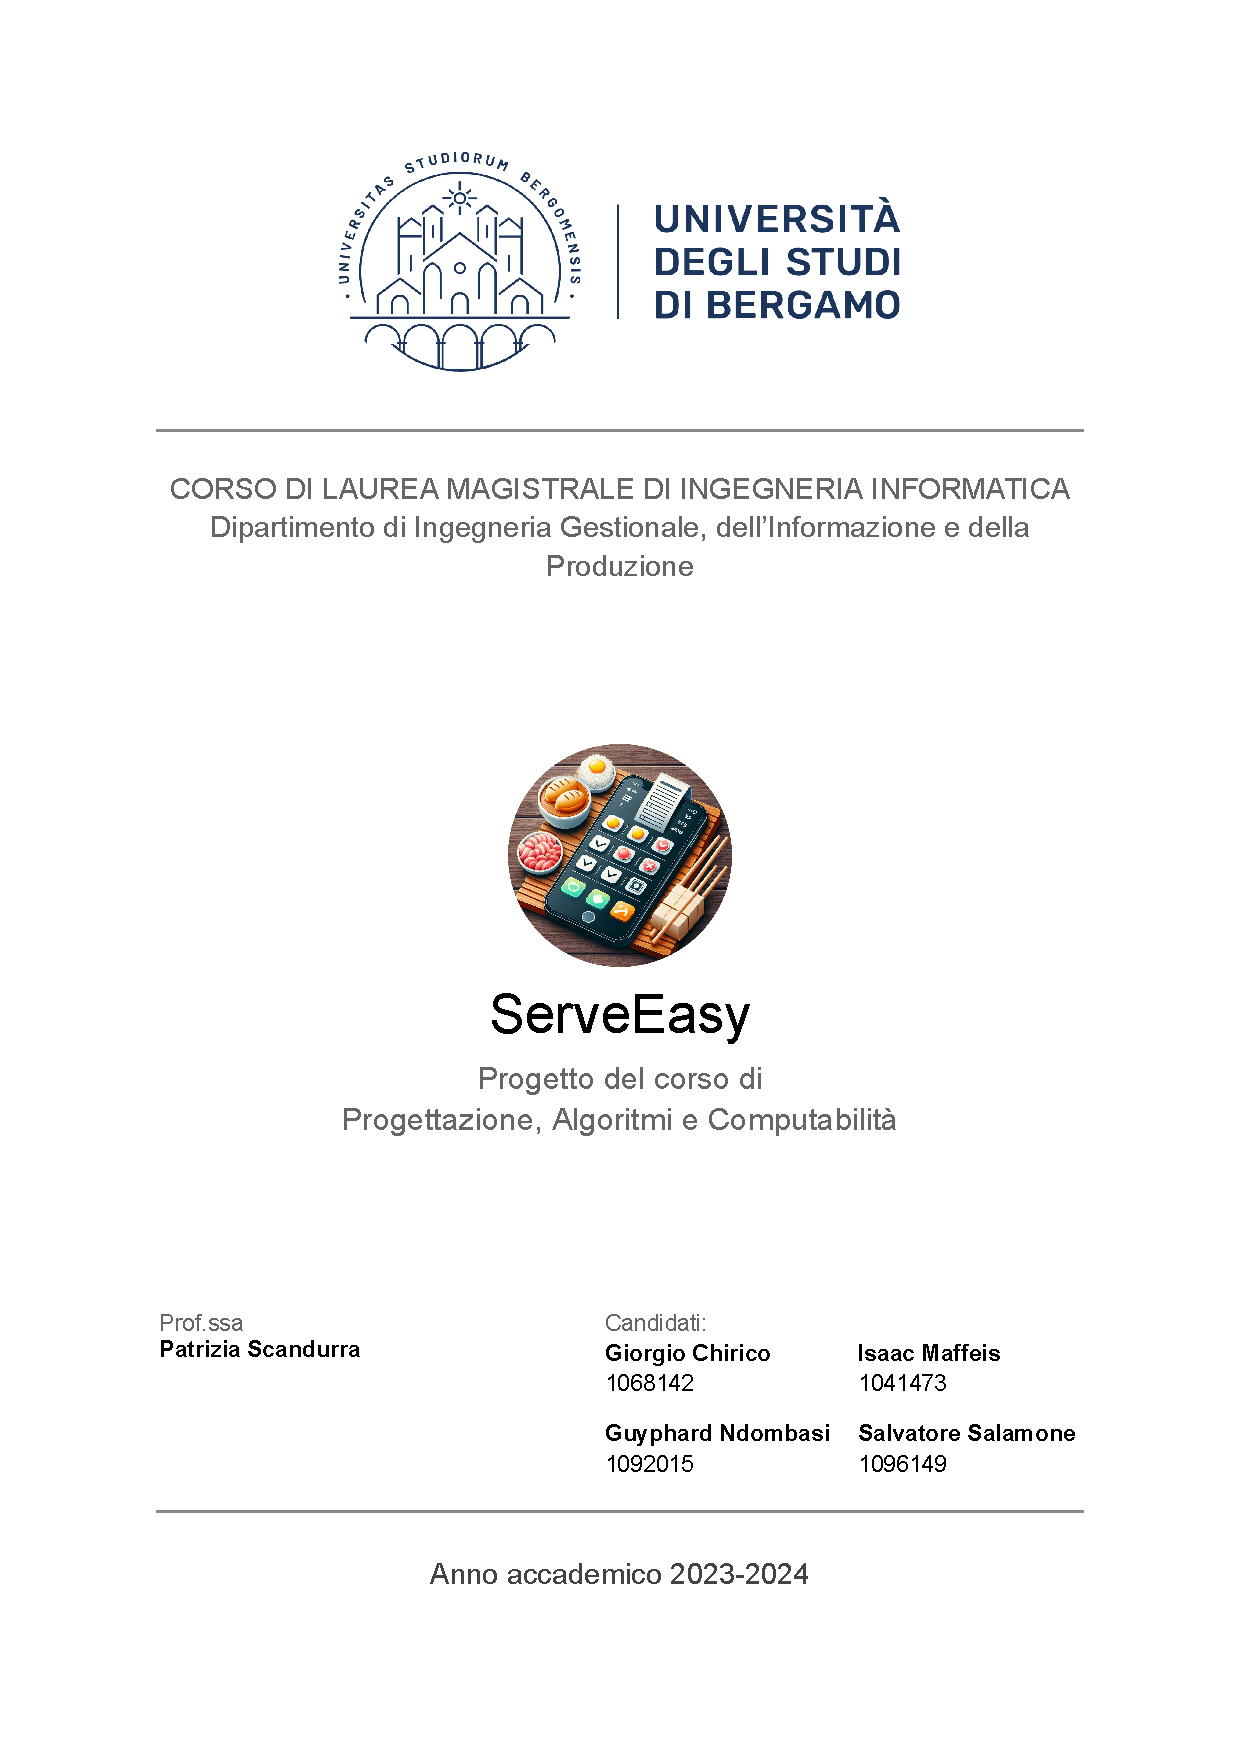
\includepdf[pages={1,{}},pagecommand={\thispagestyle{empty}}]{resources/Frontespizio.pdf}
%	\input{inizio/sommario}
	\mainmatter				
	\tableofcontents	% indice generale
	\listoffigures		% indice delle figure
	\lstlistoflistings  %indice del codice
	\addcontentsline{toc}{chapter}{Elenco dei codici}
	\chapter{Iterazione 0}
	\section{Introduzione}
Nella Iterazione 2 ci si è focalizzati a studiare l'algoritmo più adatto per la nostra applicazione, partendo dall'organizzare le entità interessate, passando poi per scrivere lo pseudo-codice ed infine ad analizzare le strutture dati necessarie.

\paragraph{Briefing} Nell'ambito di questa applicazione si considera che ogni piatto sia composto da un ingrediente principale e da più ingredienti secondari.
Ogni piatto ordinato viene chiamato ordine, quindi un ordine comprende un singolo piatto, mentre la comanda contiene tutti gli ordini di un singolo cliente.
Nel corso di un brainstorming, si è maturata l’idea di organizzare la cucina in postazioni, ognuna focalizzata su un ingrediente principale: ogni postazione si occuperà quindi di preparare e completare piatti accomunati dallo stesso ingrediente principale.
\clearpage
	\section{Requisiti funzionali}

%\subsection{Use Case Stories}

I requisiti funzionali sono stati esplicitati mediante le \textit{use case stories}, considerando come attori coinvolti nel sistema: 
\begin{itemize}
	\item Amministratore;
	\item Cliente;
	\item Cuoco;
	\item Cassiere.
\end{itemize}


\subsection{Use case stories: Amministratore}
L’amministratore è un responsabile di sala, col compito di configurare il software nelle fasi di setup dell’attività.
\subsubsection{CONFIGURAZIONE DISPOSITIVI SALA} 
\begin{itemize}
	\item Come amministratore, voglio poter registrare i dispositivi destinati ai tavoli dei clienti per consentire ai commensali di accedere al sistema;
	\item Come amministratore, voglio poter registrare i dispositivi destinati alla cucina per permettere alla cucina di gestire gli ordini;
	\item Come amministratore, voglio poter registrare un dispositivo destinato al cassiere affinché sia possibile elencare al cliente la comanda che ha ordinato.
\end{itemize}

\subsubsection{LOGIN/LOGOUT} 
\begin{itemize}
	\item Come amministratore, voglio poter effettuare il log-in/log-out dal sistema.
\end{itemize}

\subsubsection{CONFIGURAZIONE MENÙ} 
\begin{itemize}
	\item Come amministratore, voglio poter effettuare una gestione del menù per visualizzare/modificare/aggiungere/eliminare portate;  
	\item Come amministratore, voglio poter aggiungere/rimuovere/modificare gli ingredienti assegnati ad una portata per dettagliare la composizione.
\end{itemize}


\subsection{Use case stories: Cliente}
Il cliente può essere di due tipi: il cliente al tavolo, che usufruisce del dispositivo posto a disposizione dal ristorante, e il cliente da asporto, che comunica la sua ordinazione al ristorante tramite un portale sulla rete.

\subsubsection{AUTENTICAZIONE} 
\begin{itemize}
	\item Come cliente, voglio che il sistema riconosca i miei ordini così che possa elaborare le informazioni relative alla mia comanda;
\end{itemize}

\subsubsection{VISUALIZZARE MENÙ} 
\begin{itemize}
	\item Come cliente, voglio poter visualizzare il menù per decidere quale pietanza ordinare.
\end{itemize}

\subsubsection{EFFETTUARE UN'ORDINAZIONE} 
\begin{itemize}
	\item Come cliente, voglio effettuare un’ordinazione per ottenere una o più pietanze; 
	\item Come cliente, voglio effettuare un’ordinazione personalizzando la pietanza desiderata per, ad esempio, togliere ingredienti non desiderati.
\end{itemize}

\subsubsection{VISUALIZZARE STATO ORDINI} 
\begin{itemize}
	\item Come cliente, voglio poter visualizzare lo stato di preparazione dei miei ordini per poter avere un feedback dalla cucina.
\end{itemize}

\subsubsection{ANNULLARE UN ORDINE} 
\begin{itemize}
	\item Come cliente, voglio annullare l’ordinazione di un piatto.
\end{itemize}

\subsubsection{MODIFICARE UN ORDINE} 
\begin{itemize}
	\item Come cliente al tavolo, voglio poter modificare un ordine già mandato verso la cucina per, ad esempio, precisare ingredienti da togliere, qualora l’ordine non fosse già in preparazione;
	\item Come cliente al tavolo, voglio poter modificare un ordine già mandato verso al cucina per, ad esempio, esigere il piatto prima (ad es., se il cliente ritiene di star aspettando troppo) o posticipare la sua preparazione.
\end{itemize}

\subsection{Use case stories: Cuoco}
Il terzo attore coinvolto è il cuoco che prepara le ordinazioni col supporto del sistema.
\subsubsection{GESTIONE PREPARAZIONE ORDINI} 
\begin{itemize}
	\item come cuoco, voglio poter gestire gli ordini effettuati dai clienti per poter eventualmente gestire la priorità di essi;
	\item come cuoco, voglio poter modificare lo stato di un piatto per avvertire il sistema di un’avvenuta preparazione.
\end{itemize}

\subsubsection{VISUALIZZAZIONE LISTA ORDINI} 
\begin{itemize}
	\item Come cuoco, voglio poter verificare lo stato degli ordini richiesti.
\end{itemize}

\subsection{Use case stories: Cassiere}
Il cassiere legge la comanda del cliente al fine di elencare le pietanze da lui ordinate, dettagliare informazioni annesse e calcolarne il conto.
\subsubsection{VISUALIZZARE COMANDA} 
\begin{itemize}
	\item Come cassiere, voglio visualizzare la comanda delle ordinazioni relativa a un determinato cliente per generare il conto.
\end{itemize}

\subsubsection{GENERAZIONE CONTO} 
\begin{itemize}
	\item Come cassiere, voglio poter generare il conto per un determinato cliente, per concludere la sua sessione nel sistema.
	
\end{itemize}


\subsection{Priorità dei casi d’uso}

Per ottimizzare il processo di sviluppo, si è deciso di categorizzare le specifiche funzionali in tabelle con tre livelli di priorità: elevata, media e bassa. Nello specifico il primo livello è assegnato alla Tabella~\ref{tab:use_cases_high_priority} a cui sono attribuiti i casi d'uso essenziali per il funzionamento dell'applicazione, i casi d'uso relativi alle funzionalità aggiuntive non critiche sono stati attribuiti alla Tabella~\ref{tab:use_cases_medium_priority} a priorità media, mentre il livello a bassa priorità che accoglie requisiti funzionali opzionali previsti per versioni successive alla Tabella~\ref{tab:use_cases_low_priority} .

\clearpage
\subsubsection{PRIORITÀ ELEVATA}

\begin{table}[htbp]
	\centering
	 \begin{tabularx}{\textwidth}{|>{\centering\arraybackslash} m{4em}| >{\raggedright\arraybackslash}X |}
		\hline
		\textbf{Codice} & \textbf{Titolo} \\ [0.5ex]
		\hline\hline
		UC1 & Gestione comanda  \\
		\hline
		UC2 & Effettuare un'ordinazione \\
		\hline
		UC3 & Visualizzare menù \\
		\hline
		UC4 & Autenticazione \\
		\hline
		UC5 & Visualizzare lista ordini \\
		\hline
		UC6 & Gestione preparazione ordini \\
		\hline
	\end{tabularx}
	\caption{Casi d'uso ad elevata priorità}
	\label{tab:use_cases_high_priority}
\end{table}

\subsubsection{PRIORITÀ MEDIA}
\begin{table}[htbp]
	\centering
	\begin{tabularx}{\textwidth}{|>{\centering\arraybackslash} m{4em}| >{\raggedright\arraybackslash}X |}
		\hline
		\textbf{Codice} & \textbf{Titolo} \\ [0.5ex]
		\hline\hline
		UC7 & Configurazione dispositivi sala \\
		\hline
		UC8 & Gestione dispositivi \\
		\hline
		UC9 & Login amministratore \\
		\hline
		UC10 & Logout amministratore \\
		\hline
		UC11 & Configurazione menù \\
		\hline
		UC12 & Gestione dati menù \\
		\hline
	\end{tabularx}
	\caption{Casi d'uso a media priorità}
	\label{tab:use_cases_medium_priority}
\end{table}

\subsubsection{PRIORITÀ BASSA}
\begin{table}[htbp]
	\centering
	\begin{tabularx}{\textwidth}{|>{\centering\arraybackslash} m{4em}| >{\raggedright\arraybackslash}X |}
		\hline
		\textbf{Codice} & \textbf{Titolo} \\ [0.5ex]
		\hline\hline
		UC13 & Modifica un ordine  \\
		\hline
		UC14 & Annullare un ordine  \\
		\hline
		UC15 & Visualizza stato delle ordinazioni \\
		\hline
		UC16 & Generazione conto   \\
		\hline
		UC17 & Visualizzare comanda   \\
		\hline
	\end{tabularx}
	\caption{Casi d'uso a bassa priorità}
	\label{tab:use_cases_low_priority}
\end{table}


\subsection{Use case diagram}

Dalla descrizione delle \textit{use case stories}, è stato creato il diagramma UML dei casi d'uso in \figurename~\ref{fig:use_cases_diagram}, il quale è composto da 4 attori (Amministratore, Cuoco, Cassiere e Cliente che tramite ereditarietà viene ridefinito in Cliente al tavolo oppure Cliente che effettua ordinazioni d’asporto) e 6 viste (vista amministratore, vista cucina, vista cassiere, vista cliente, vista cliente al tavolo e sistema).

\begin{figure}[htbp]
	\begin{comment}
		The [htbp] option in LaTeX is used to fine-tune the placement of tables and figures.
		Each letter in [htbp] stands for a particular placement option:
		h (here): Place the table or figure in the text where the environment (like figure or table) is written, if there is enough room left on the page.
		t (top): Place it at the top of a page.
		b (bottom): Place it at the bottom of a page.
		p (page): Place it on a page containing only floats, such as figures and tables	
		LaTeX will try to place the float at the location that comes first in the option list.
		If it can’t place it there due to constraints like page size, it will move on to the next option. If none of the specified options work, LaTeX will hold the float until it finds a place where it fits, or until a \clearpage command is encountered
	\end{comment}
	\centering
	
	% verticale
	%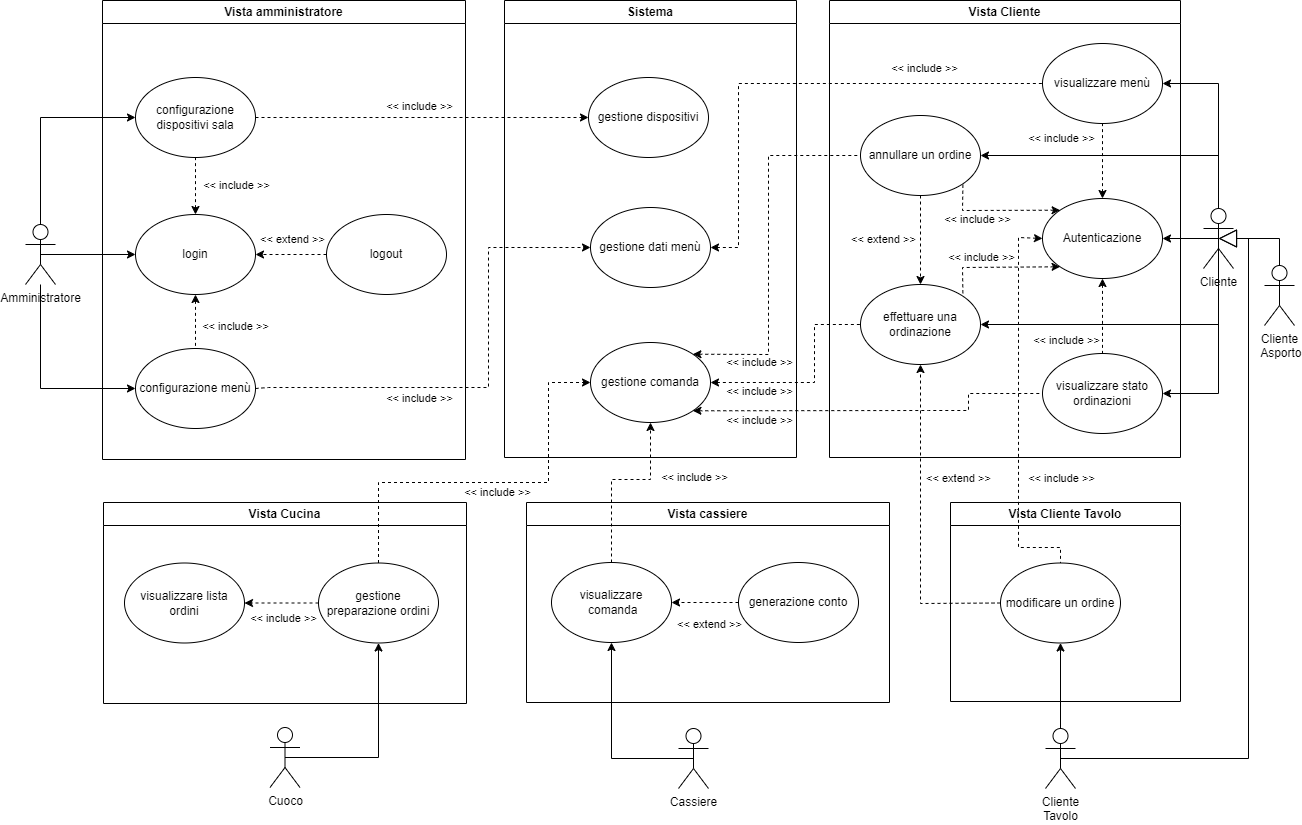
\includegraphics[scale=0.4, angle=90]{iterazione0/images/use_cases_diagram}
	
	% orizzontale
	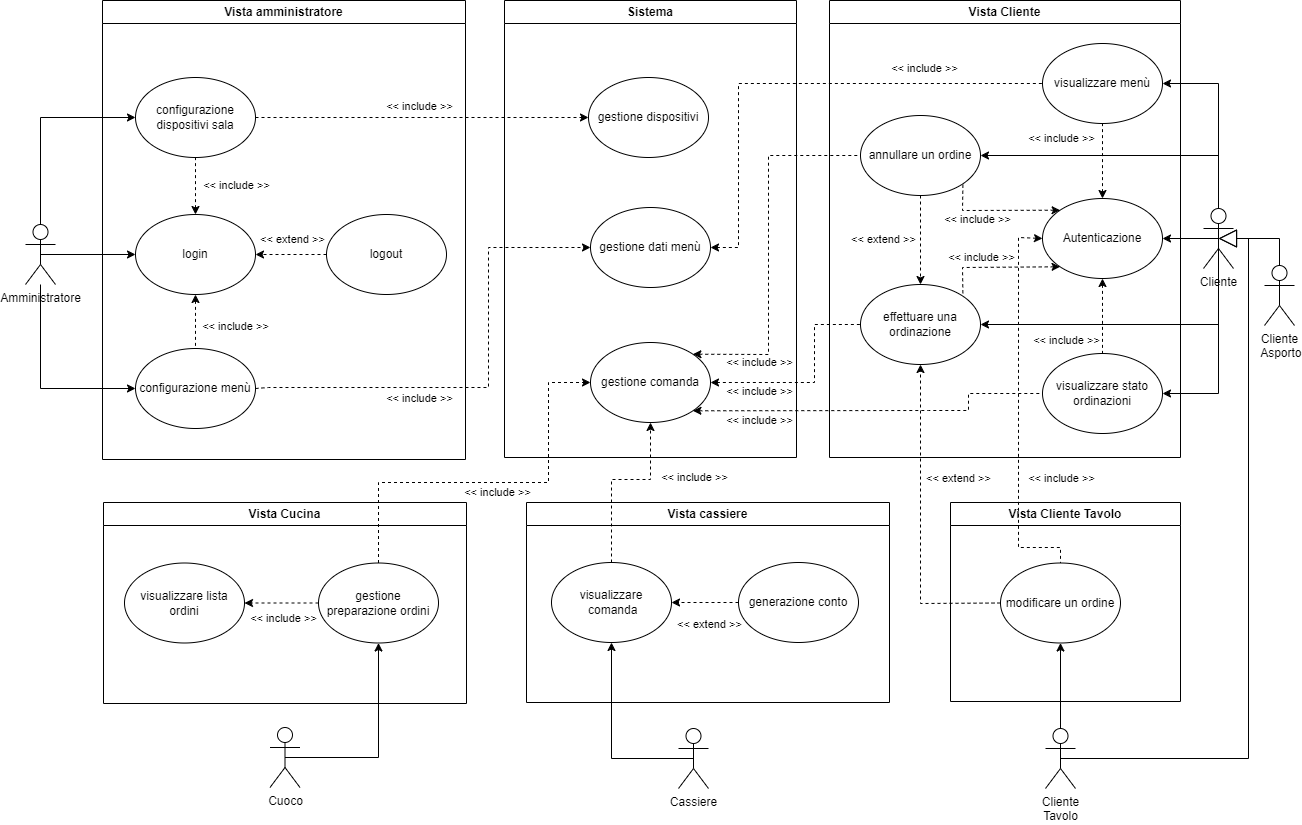
\includegraphics[scale=0.32]{iterazione0/images/use_cases_diagram}
	\caption{Diagramma dei casi d'uso\label{fig:use_cases_diagram}}
\end{figure}

\clearpage
	\section{Requisiti non funzionali}
Il progetto verrà sviluppato tenendo considerazione delle performance, integrabilità, modificabilità, testabilità e sicurezza dei componenti.

\subsection{Performance}
L'algoritmo di priorità impiegato dalla cucina per la selezione degli ordini deve fornire risultati in un tempo utile. Allo stesso tempo, gli utenti dell'applicativo web devono poter accedere e aggiornare le informazioni in un tempo accettabile.

\subsection{Integrabilità}
Ogni componente di sistema deve collaborare con gli altri componenti in modo da garantire le funzionalità previste dal sistema. Questa caratteristica è essenziale per garantire il corretto funzionamento e la coerenza dell'intero sistema.

\subsection{Modificabilità}
Il software deve facilitare l’aggiunta di nuovi componenti e funzionalità.

\subsection{Testabilità}
Ogni componente deve poter permettere la progettazione, implementazione ed esecuzione di test efficaci, in modo da garantire una massima copertura di requisiti e funzionalità.

\subsection{Sicurezza}
Il sistema deve integrare meccanismi di autenticazione ed autorizzazione degli attori, in modo da garantire la gestione delle identità, oltre alla protezione dei dati e delle API da accessi non autorizzati. Risulta dunque necessaria una distinzione dei ruoli con cui gli attori accedono al sistema.

\clearpage
	\section{Topologia}
Per il progetto è stata adottata una topologia three-tier al fine di separare in tre livelli distinti la presentazione dei dati, la gestione dell’applicativo e la mappatura dei dati sui dispositivi di archiviazione. Come si può vedere dalla \figurename~\ref{fig:topologia} il servizio è esposto tramite un web server, al quale i dispositivi clienti accedono, tramite richiesta HTTP/REST, per mezzo di una API unificata, con funzionalità di gateway. Il web-server usufruirà di database relazionali per lo storage (Data Layer), mentre sarà supportato da un database in-memory H2 (Application Layer) per avvantaggiarsi di una ridondanza dati, allo scopo di aumentare le performance lato client.

\begin{figure}[htbp]
	\centering
	
	% orizzontale
	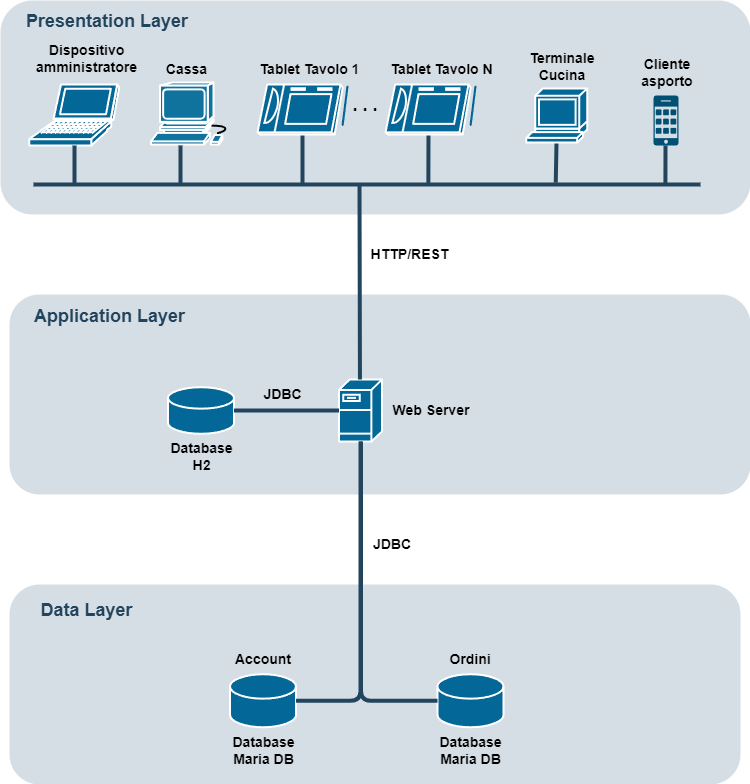
\includegraphics[scale=0.5]{iterazione0/images/topologia}
	\caption{Topologia del sistema\label{fig:topologia}}
\end{figure}

\clearpage
	\section{Toolchain}
Di seguito è presentata la toolchain utilizzata per lo sviluppo del progetto software
\subsection{Modellazione}
\begin{itemize}
	\item draw.io: casi d’uso e topologia;
\end{itemize}

\subsection{Stack applicativo}
\begin{itemize}
	\item Angular.js: front-end;
	\item Java Spring Boot 3.x.x: back-end;
	\item MariaDB: database per l’archiviazione;
	\item H2: database in-memory per rendere più efficiente l’estrazione dei dati;
\end{itemize}

\subsection{Deployment}
\begin{itemize}
	\item Docker: piattaforma per container virtuali;
	\item Docker Compose: gestione app multi-container;
\end{itemize}

\subsection{Gestore repository}
\begin{itemize}
	\item Git: Controllo versione per codice sorgente;
	\item GitHub: Piattaforma hosting e collaborativa per progetti Git;
\end{itemize}

\subsection{Continuous Integration}
\begin{itemize}
	\item Maven: gestore di progetti e dipendenze Java;
	\item GitHub Action: piattaforma di automazione per repository GitHub;
	\item Jenkins: strumento di automazione per sviluppatori;
\end{itemize}

\subsection{Analisi statica}
\begin{itemize}
	\item Checkstyle: visualizzazione di alto livello di metriche qualitative del codice;
\end{itemize}

\subsection{Analisi dinamica}
\begin{itemize}
	\item Postman: strumento per testare API e servizi;
	\item Garfana: analisi delle performance della rete di microservizi;
	\item JUNIT: framework per test unitari Java;
\end{itemize}

\subsection{Documentazione e organizzazione del team}
\begin{itemize}
	\item Google Drive: servizio cloud per archiviazione;
	\item Documenti condivisi di Google: per elaborare la documentazione in modo condiviso;
	\item \LaTeX: generazione documentazione;
	\item Microsoft Teams: per organizzazione e meeting;
\end{itemize}

\subsection{Modello di sviluppo}
Il modello adottato segue la filosofia AGILE, con enfasi sui seguenti aspetti-chiave:
\begin{itemize}
	\item pair programming, per favorire creatività e controllo del lavoro prodotto;
	\item orientamento al risultato, con enfasi maggiore sulla generazione di codice funzionante e componenti completi prima della relativa documentazione;
	\item rapidità di risposta ai cambiamenti;
	\item collaborazione attiva col cliente, al fine di incontrare le sue necessità, garantire trasparenza e fornire feedback tempestivo sul lavoro di progetto;
	\item Proattività nell’identificazione e mitigazione dei rischi.
\end{itemize}

\clearpage
	\chapter{Iterazione 1}
	\section{Introduzione}
Nella Iterazione 2 ci si è focalizzati a studiare l'algoritmo più adatto per la nostra applicazione, partendo dall'organizzare le entità interessate, passando poi per scrivere lo pseudo-codice ed infine ad analizzare le strutture dati necessarie.

\paragraph{Briefing} Nell'ambito di questa applicazione si considera che ogni piatto sia composto da un ingrediente principale e da più ingredienti secondari.
Ogni piatto ordinato viene chiamato ordine, quindi un ordine comprende un singolo piatto, mentre la comanda contiene tutti gli ordini di un singolo cliente.
Nel corso di un brainstorming, si è maturata l’idea di organizzare la cucina in postazioni, ognuna focalizzata su un ingrediente principale: ogni postazione si occuperà quindi di preparare e completare piatti accomunati dallo stesso ingrediente principale.
\clearpage
	\section{Use Cases}

Si sono presi in considerazione i seguenti casi d'uso, ossia quelli a priorità più elevata della Tabella~\ref{tab:use_cases_high_priority}

\begin{table}[htbp]
	\centering
	\begin{tabularx}{\textwidth}{|>{\centering\arraybackslash} m{4em}| >{\raggedright\arraybackslash}X |}
		\hline
		\textbf{Codice} & \textbf{Titolo} \\ [0.5ex]
		\hline\hline
		UC1 & Gestione comanda  \\
		\hline
		UC2 & Effettuare un'ordinazione \\
		\hline
		UC3 & Visualizzare menù \\
		\hline
		UC4 & Autenticazione \\
		\hline
		UC5 & Visualizzare lista ordini \\
		\hline
		UC6 & Gestione preparazione ordini \\
		\hline
	\end{tabularx}
	\caption{Casi d'uso presi in considerazione nell'iterazione 1}
	\label{tab:use_cases_it1}
\end{table}

\begin{figure}[htbp]
	\centering
	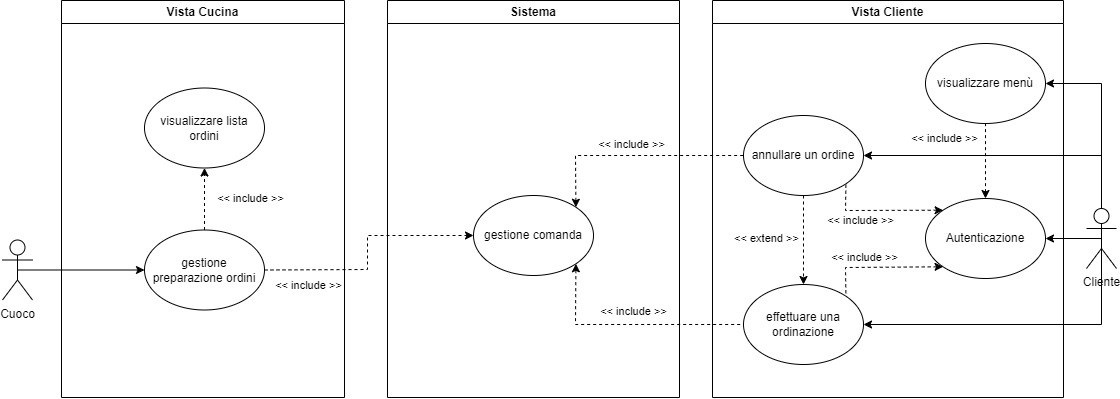
\includegraphics[scale=0.36]{iterazione1/images/useCases_it1.jpg}
	\caption{Casi d'uso presi in considerazione nell'iterazione 1\label{fig:use_cases_it1}}
\end{figure}

Per facilitare una migliore organizzazione e comprensione del sistema, i casi d'uso vengono raggruppati nel seguente modo:

\subsection{Gruppo Sistema}
\paragraph{UC-1 “Gestione Comanda”:}
\begin{itemize}
	\item UC-1.1 : gestione priorità ordine \\ ogni ordine è caratterizzato da una priorità
	\item UC-1.2 : gestione coda ordini \\
	ogni ordine è inserito in una coda ordini
	\item UC-1.3 : assegnazione ordini comanda \\
	ogni ordine deve essere associato ad una comanda
	\item UC-1.4 : assegnazione comanda cliente \\
	ogni comanda deve essere associata ad un cliente
\end{itemize}

\subsection{Gruppo cliente}
\paragraph{UC-2 “effettuare un’ordinazione”:}
\begin{itemize}
	\item UC-2.1 : effettuare un ordine personalizzato \\
	il cliente può effettuare un ordine escludendo un ingrediente o descrivendo una variazione del piatto
\end{itemize}

\paragraph{UC-3 “Visualizzare menu”:}
\begin{itemize}
	\item UC-3.1 : visualizzare piatto 
	\item UC-3.2 : visualizzare informazioni piatto \\
	il cliente deve poter leggere breve descrizione, ingredienti, prezzo
\end{itemize}

\paragraph{UC-4 “Autenticazione”:}
\begin{itemize}
	\item UC-4.1 : identificazione sessione cliente \\ 
	al momento del pasto e solo per il pasto, il cliente deve poter distinguere la propria comanda
\end{itemize}

\subsection{Gruppo cuoco}
\paragraph{UC-5 “visualizzare lista ordini”:}
\begin{itemize}
	\item UC-5.1 : visualizzazione ordini per postazione \\ 
	il cuoco deve visualizzare gli ordini destinati alla sua postazione
\end{itemize}

\paragraph{UC-6 “gestione preparazione ordini”:}
\begin{itemize}
	\item UC-6.1 : notifica preparazione ordine \\ 
	il cuoco deve segnalare la presa in carico dell’ordine
	\item UC-6.2 : notifica completamento ordine \\
	il cuoco deve segnalare il completamento dell’ordine così da passare al successivo
	\item UC-6.3 : gestione priorità postazione \\
	il cuoco può modificare la priorità di un certo ingrediente così da ridurre la pressione su una certa postazione o, viceversa, per aumentarne il traffico. In tal modo può manualmente agire sulla gestione del traffico verso la cucina.
\end{itemize}

\clearpage
	\section{Component Diagram}
\subsection{Sistema ServeEasy}
\subsubsection{single component del sistema}
\begin{figure}[H]
	\centering
	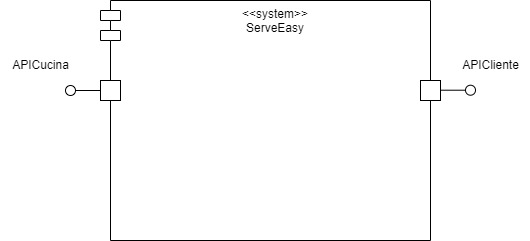
\includegraphics[scale=0.6]{iterazione1/images/ServeEasy_componente_unico.jpg}
	\caption{Component diagram - ServeEasy\label{fig:component_diagram_serveeasy}}
\end{figure}
Visualizzazione iniziale della soluzione come un componente unico che espone due API, dedicate rispettivamente alla cucina ed ai clienti. Si procede con uno sviluppo top-down.

\subsubsection{primo zoom-in sul sistema}

\begin{figure}[H]
	\centering
	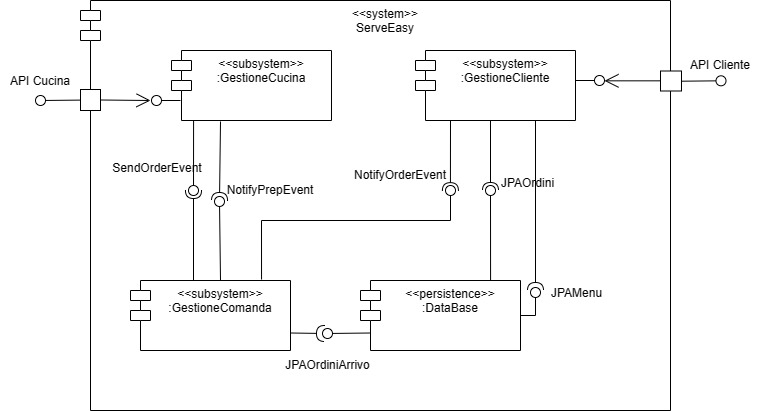
\includegraphics[scale=0.5]{iterazione1/images/ServeEasy_primo_zoomin.jpg}
	\caption{Component diagram - System\label{fig:component_diagram_system}}
\end{figure}
Al primo zoom-in si identificano i servizi che andranno a comporre l’architettura della soluzione:
\begin{itemize}
	\item \textbf{GestioneComanda:} risolve gli use case del gruppo “sistema”, rappresenta il cuore del sistema ed incorpora la logica di backend fondamentale per la gestione regolarizzata degli ordini da cliente a cucina, attraverso politiche di schedulazione a priorità progettate ed implementate con un algoritmo ad-hoc.
	\item \textbf{GestioneCliente:} risolve gli use case del gruppo “cliente”, espone le funzionalità destinate ai dispositivi di tavolo ed al portale web per clienti d’asporto. Ha dunque il compito di gestire gli aspetti del servizio legati alle interazioni del cliente col sistema, come la visualizzazione del menu, la creazione degli ordini ed il raggruppamento degli ordini in una comanda relativa.
	\item \textbf{GestioneCucina:} risolve gli use case del gruppo “cucina”, espone le chiamate destinate ai dispositivi di cucina. Questo servizio conterrà un sistema a code, dove l’ordine in arrivo verrà classificato ed inserito in base al suo ingrediente principale. Gli ordini verranno gestiti dalle postazioni della cucina seguendo una politica FIFO.
\end{itemize}
Per la memorizzazione persistente dei dati cruciali per l’attività come piatti, ordini e comande, è stato inserito un componente database.
All’interno del sistema ServeEasy, i componenti comunicano tra loro attraverso una comunicazione ad eventi, asincrona. Si è deciso di attuare una politica pub-sub per la gestione delle comunicazioni interne, costituite da scambi di notifiche e DTO tra i microservizi designati.

\subsection{Gestione Comanda}
\subsubsection{Componenti esagonali}
Il design dei microservizi seguirà l’architettura esagonale: un dominio, denominato “Domain”, nucleo della logica di servizio, sarà racchiuso tra due gusci denominati “Interface” e “Infrastructure”, i quali avranno il compito di astrarre la gestione dati, rendendola opaca al dominio. La logica di base del microservizio seguirà lo schema port-adapter, dove il dominio comunica con i gusci attraverso delle interfacce dette porte (il cui nome nel progetto è caratterizzato dal suffisso “Port”), mentre i gusci hanno il compito di implementare l’effettivo componente di trasmissione (guscio Infrastructure) e/o ricezione (guscio Interface), detto adattatore (sarà identificabile da suffisso “Adapter”). 
Nello specifico il \textbf{Domain} definisce gli oggetti, le entità e le operazioni che sono pertinenti al problema che il microservizio gestisce.Gli \textbf{Interface adapters} fungono da ponte tra il mondo esterno e il core del sistema, consentendo al microservizio di comunicare con altre applicazioni, servizi o dispositivi esterni in modo indipendente dall'implementazione interna del sistema stesso, mentre gli \textbf{Infrastructure adapters} fungono da ponte tra il core del sistema e l'infrastruttura esterna, gestendo le chiamate e le operazioni necessarie per accedere e utilizzare le risorse infrastrutturali.
Tali caratteristiche avvantaggiano l’intercambiabilità dei singoli componenti di sistema a costo di un aumento della complessità.
\begin{figure}[H]
	\centering
	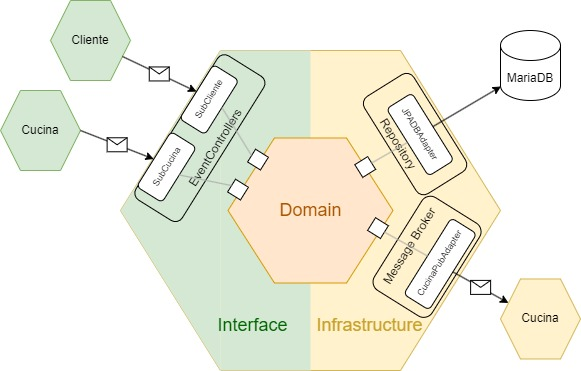
\includegraphics[scale=0.7]{iterazione1/images/hexagon.jpg}
	\caption{Architettura esagonale per il microservizio Gestione comanda\label{fig:hexagon}}
\end{figure}

\subsubsection{zoom-in gestione comanda}
\begin{figure}[H]
	\centering
	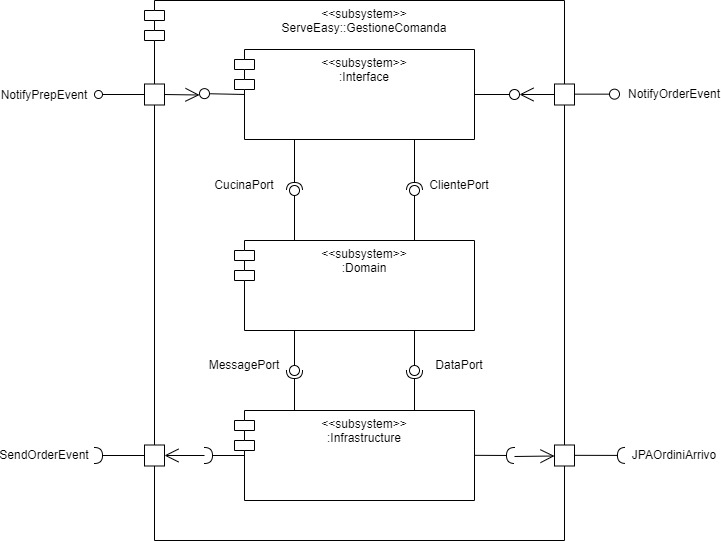
\includegraphics[scale=0.5]{iterazione1/images/component_comanda_cucina-GestioneComanda.jpg}
	\caption{Component diagram - Gestione Comanda\label{fig:component_diagram_gestione_comanda}}
\end{figure}


\subsubsection{zoom-in infrastructure di gestione comanda}
\begin{figure}[H]
	\centering
	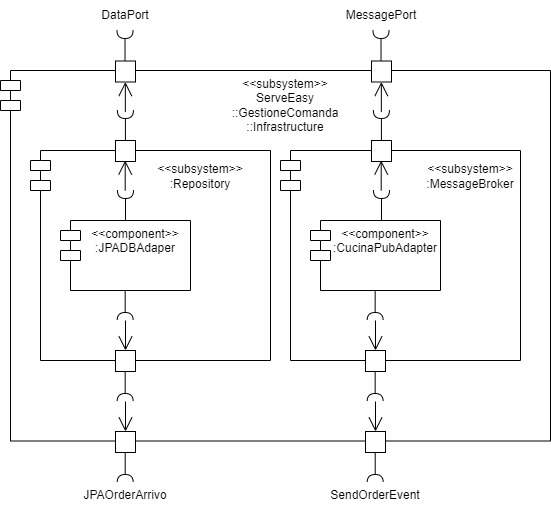
\includegraphics[scale=0.5]{iterazione1/images/component_comanda_cucina-GestioneComanda__Infrastructure.jpg}
	\caption{Component diagram - Gestione Comanda - Infrasrtructure \label{fig:component_diagram_gestione_comanda_infrastracture}}
\end{figure}
\begin{itemize}
    \item Repository: JPADBAdapter per la comunicazione con il database;
    \item MessageBroker: CucinaPubAdapter per l'invio di messaggi sul topic verso il microservizio della cucina.
\end{itemize}

\subsubsection{zoom-in domain di gestione comanda}
\begin{figure}[H]
	\centering
	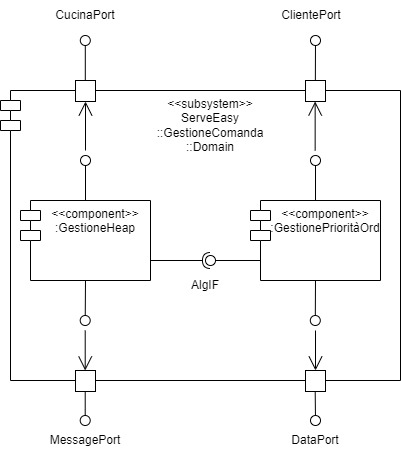
\includegraphics[scale=0.5]{iterazione1/images/component_comanda_cucina-GestioneComanda__Domain.jpg}
	\caption{Component diagram - Gestione Comanda - Domain \label{fig:component_diagram_gestione_comanda_domain}}
\end{figure}

\subsubsection{zoom-in interface di gestione comanda}
\begin{figure}[H]
	\centering
	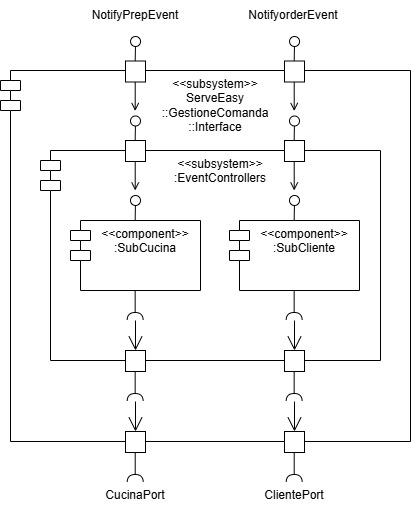
\includegraphics[scale=0.5]{iterazione1/images/component_comanda_cucina-GestioneComanda__Interface.jpg}
	\caption{Component diagram - Gestione Comanda - Interface \label{fig:component_diagram_gestione_comanda_interface}}
\end{figure}
\begin{itemize}
    \item EventControllers: SubCucina e SubCliente, permettono la ricezione di messaggi tramite message broker dagli altri microservizi.
\end{itemize}

\subsection{Gestione Cliente}
\subsubsection{zoom-in gestione cliente}
\begin{figure}[H]
	\centering
	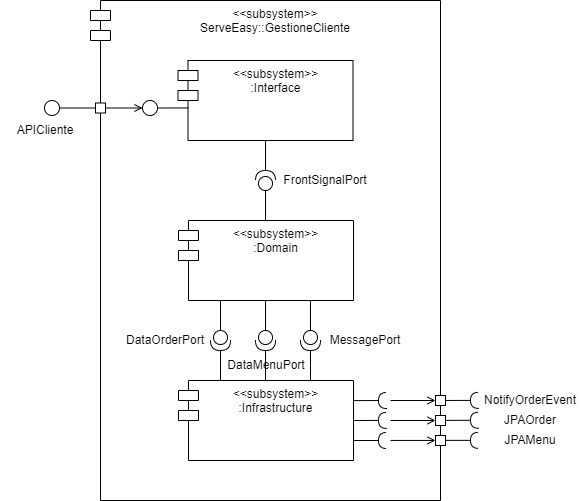
\includegraphics[scale=0.5]{iterazione1/images/GestioneCliente_subsystem-GestioneCliente.jpg}
	\caption{Component diagram - Gestione Cliente \label{fig:component_diagram_gestione_cliente}}
\end{figure}

\subsubsection{zoom-in infrastructure di gestione cliente}
\begin{figure}[H]
	\centering
	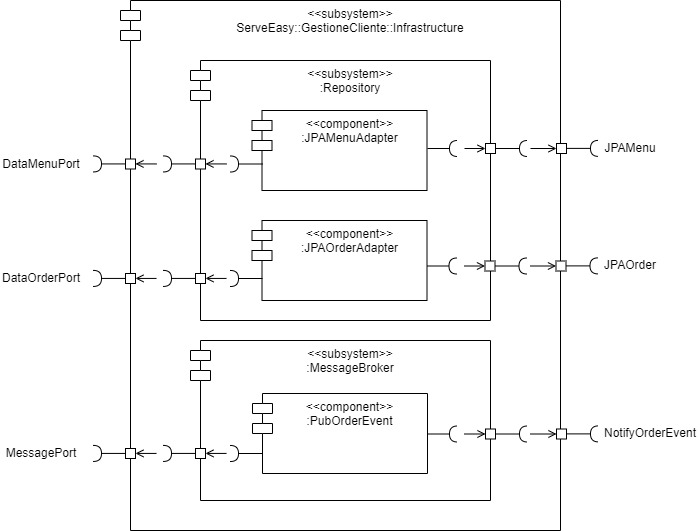
\includegraphics[scale=0.5]{iterazione1/images/GestioneCliente_subsystem-Infrastructure.jpg}
	\caption{Component diagram - Gestione Cliente - Infrastructure \label{fig:component_diagram_gestione_cliente_infrastructure}}
\end{figure}
\begin{itemize}
    \item Repository: JPAOrderAdapter e JPAMenuAdapter per la comunicazione con il database;
    \item MessageBroker: PubOrderEvent per l'invio di messaggi sul topic verso il microservizio della cucina.
\end{itemize}

\subsubsection{zoom-in domain di gestione cliente}
\begin{figure}[H]
	\centering
	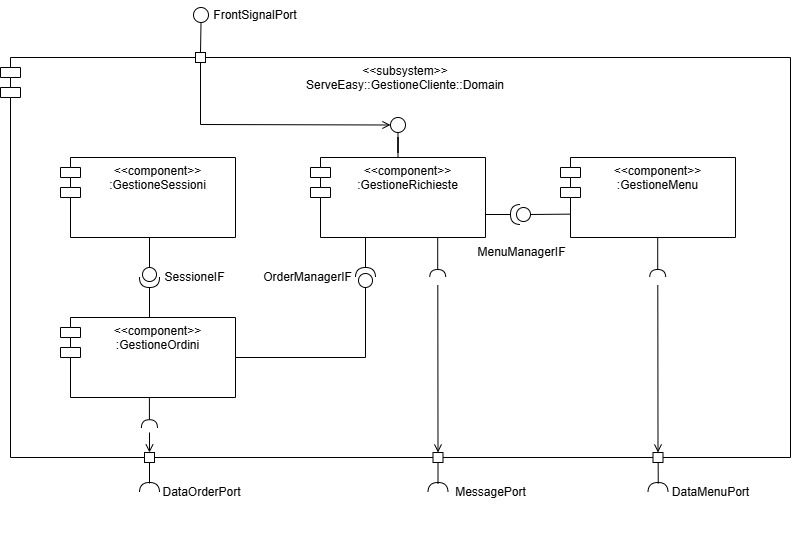
\includegraphics[scale=0.5]{iterazione1/images/GestioneCliente_subsystem-Domain.jpg}
	\caption{Component diagram - Gestione Cliente - Domain \label{fig:component_diagram_gestione_cliente_domain}}
\end{figure}

\subsubsection{zoom-in interface di gestione cliente}
\begin{figure}[H]
	\centering
	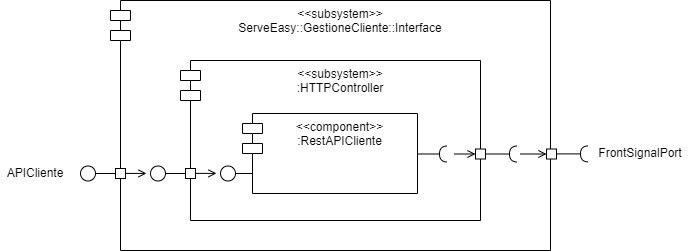
\includegraphics[scale=0.5]{iterazione1/images/GestioneCliente_subsystem-Interface.jpg}
	\caption{Component diagram - Gestione Cliente - Interface \label{fig:component_diagram_gestione_cliente_interface}}
\end{figure}
\begin{itemize}
    \item HTTPControllers: RestApiCliente, permette di esporre API verso l'esterno.
\end{itemize}

\subsection{Gestione Cucina}
\subsubsection{zoom-in gestione cucina}
\begin{figure}[H]
	\centering
	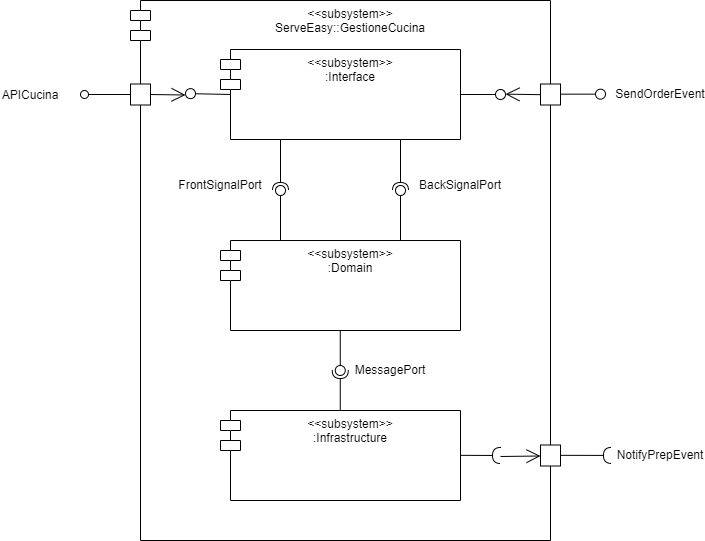
\includegraphics[scale=0.5]{iterazione1/images/component_comanda_cucina-GestioneCucina.jpg}
	\caption{Component diagram - Gestione Cucina \label{fig:component_diagram_gestione_cucina}}
\end{figure}

\subsubsection{zoom-in infrastructure di gestione cucina}
\begin{figure}[H]
	\centering
	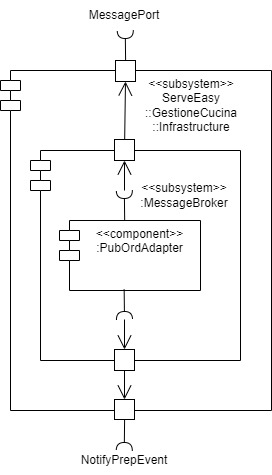
\includegraphics[scale=0.5]{iterazione1/images/component_comanda_cucina-GestioneCucina__Infrastructure.jpg}
	\caption{Component diagram - Gestione Cucina - Infrastructure \label{fig:component_diagram_gestione_cucina_infrastructure}}
\end{figure}
\begin{itemize}
    \item Repository: JPADBAdapter per la comunicazione con il database;
    \item MessageBroker: PubOrderAdapter per l'invio di messaggi sul topic verso il microservizio di GestioneComanda.
\end{itemize}

\subsubsection{zoom-in domain di gestione cucina}
\begin{figure}[H]
	\centering
	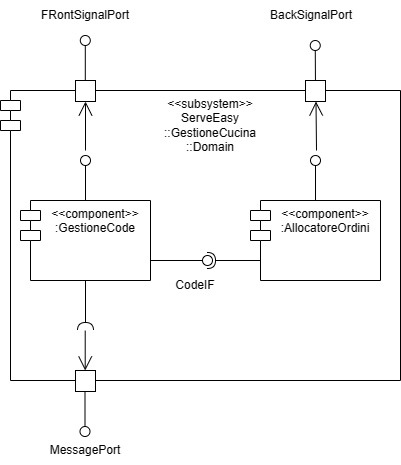
\includegraphics[scale=0.5]{iterazione1/images/component_comanda_cucina-GestioneCucina__Domain.jpg}
	\caption{Component diagram - Gestione Cucina - Domain \label{fig:component_diagram_gestione_cucina_domain}}
\end{figure}

\subsubsection{zoom-in interface di gestione cucina}
\begin{figure}[H]
	\centering
	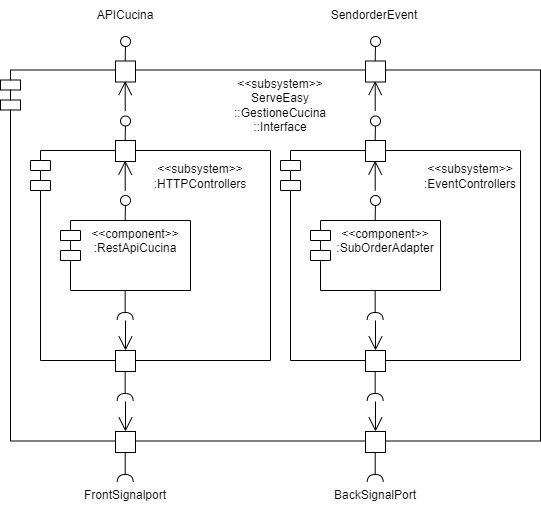
\includegraphics[scale=0.5]{iterazione1/images/component_comanda_cucina-GestioneCucina__Interface.jpg}
	\caption{Component diagram - Gestione Cucina - Interface \label{fig:component_diagram_gestione_cucina_interface}}
\end{figure}
\begin{itemize}
    \item EventControllers: SubOrderAdapter, permette la ricezione di messaggi tramite message broker dal microservizio GestioneComanda;
    \item HTTPControllers: RestApiCucina, permette di esporre API verso l'esterno.
\end{itemize}



\clearpage
	\section{Database}
Per facilitare l'identificazione delle entità coinvolte nel database si è utilizzato un modello entità-relazione che fornisce una rappresentazione grafica chiara e intuitiva della struttura dei dati. Questo modello aiuta a visualizzare le entità (oggetti o concetti del mondo reale), le relazioni (le associazioni tra le entità) e gli attributi (le proprietà o le caratteristiche delle entità e delle relazioni).
\subsection{Modello Entità-Relazione}
Nel seguente diagramma entità-relazione in Figura~\ref{fig:er_diagram}, osserviamo che le comande possono essere costituite da più ordini effettuati dai clienti. Tali clienti sono suddivisi in due categorie: clienti d’asporto identificati tramite numero di telefono e clienti al tavolo identificati tramite numero del tavolo. I piatti, consultabili tramite un menù, sono caratterizzati da un ingrediente principale. Una volta ordinato un piatto dal menù, questo viene inserito al’interno di un ordine identificato da un codice progressivo per cliente, e viene successivamente inserito nella comanda del rispettivo cliente. La comanda sarà quindi utilizzata per identificare il cliente e contiene i piatti ordinati oltre che il totale dello scontrino con il corrispettivo codice di pagamento.

\begin{figure}[H]
	\centering
	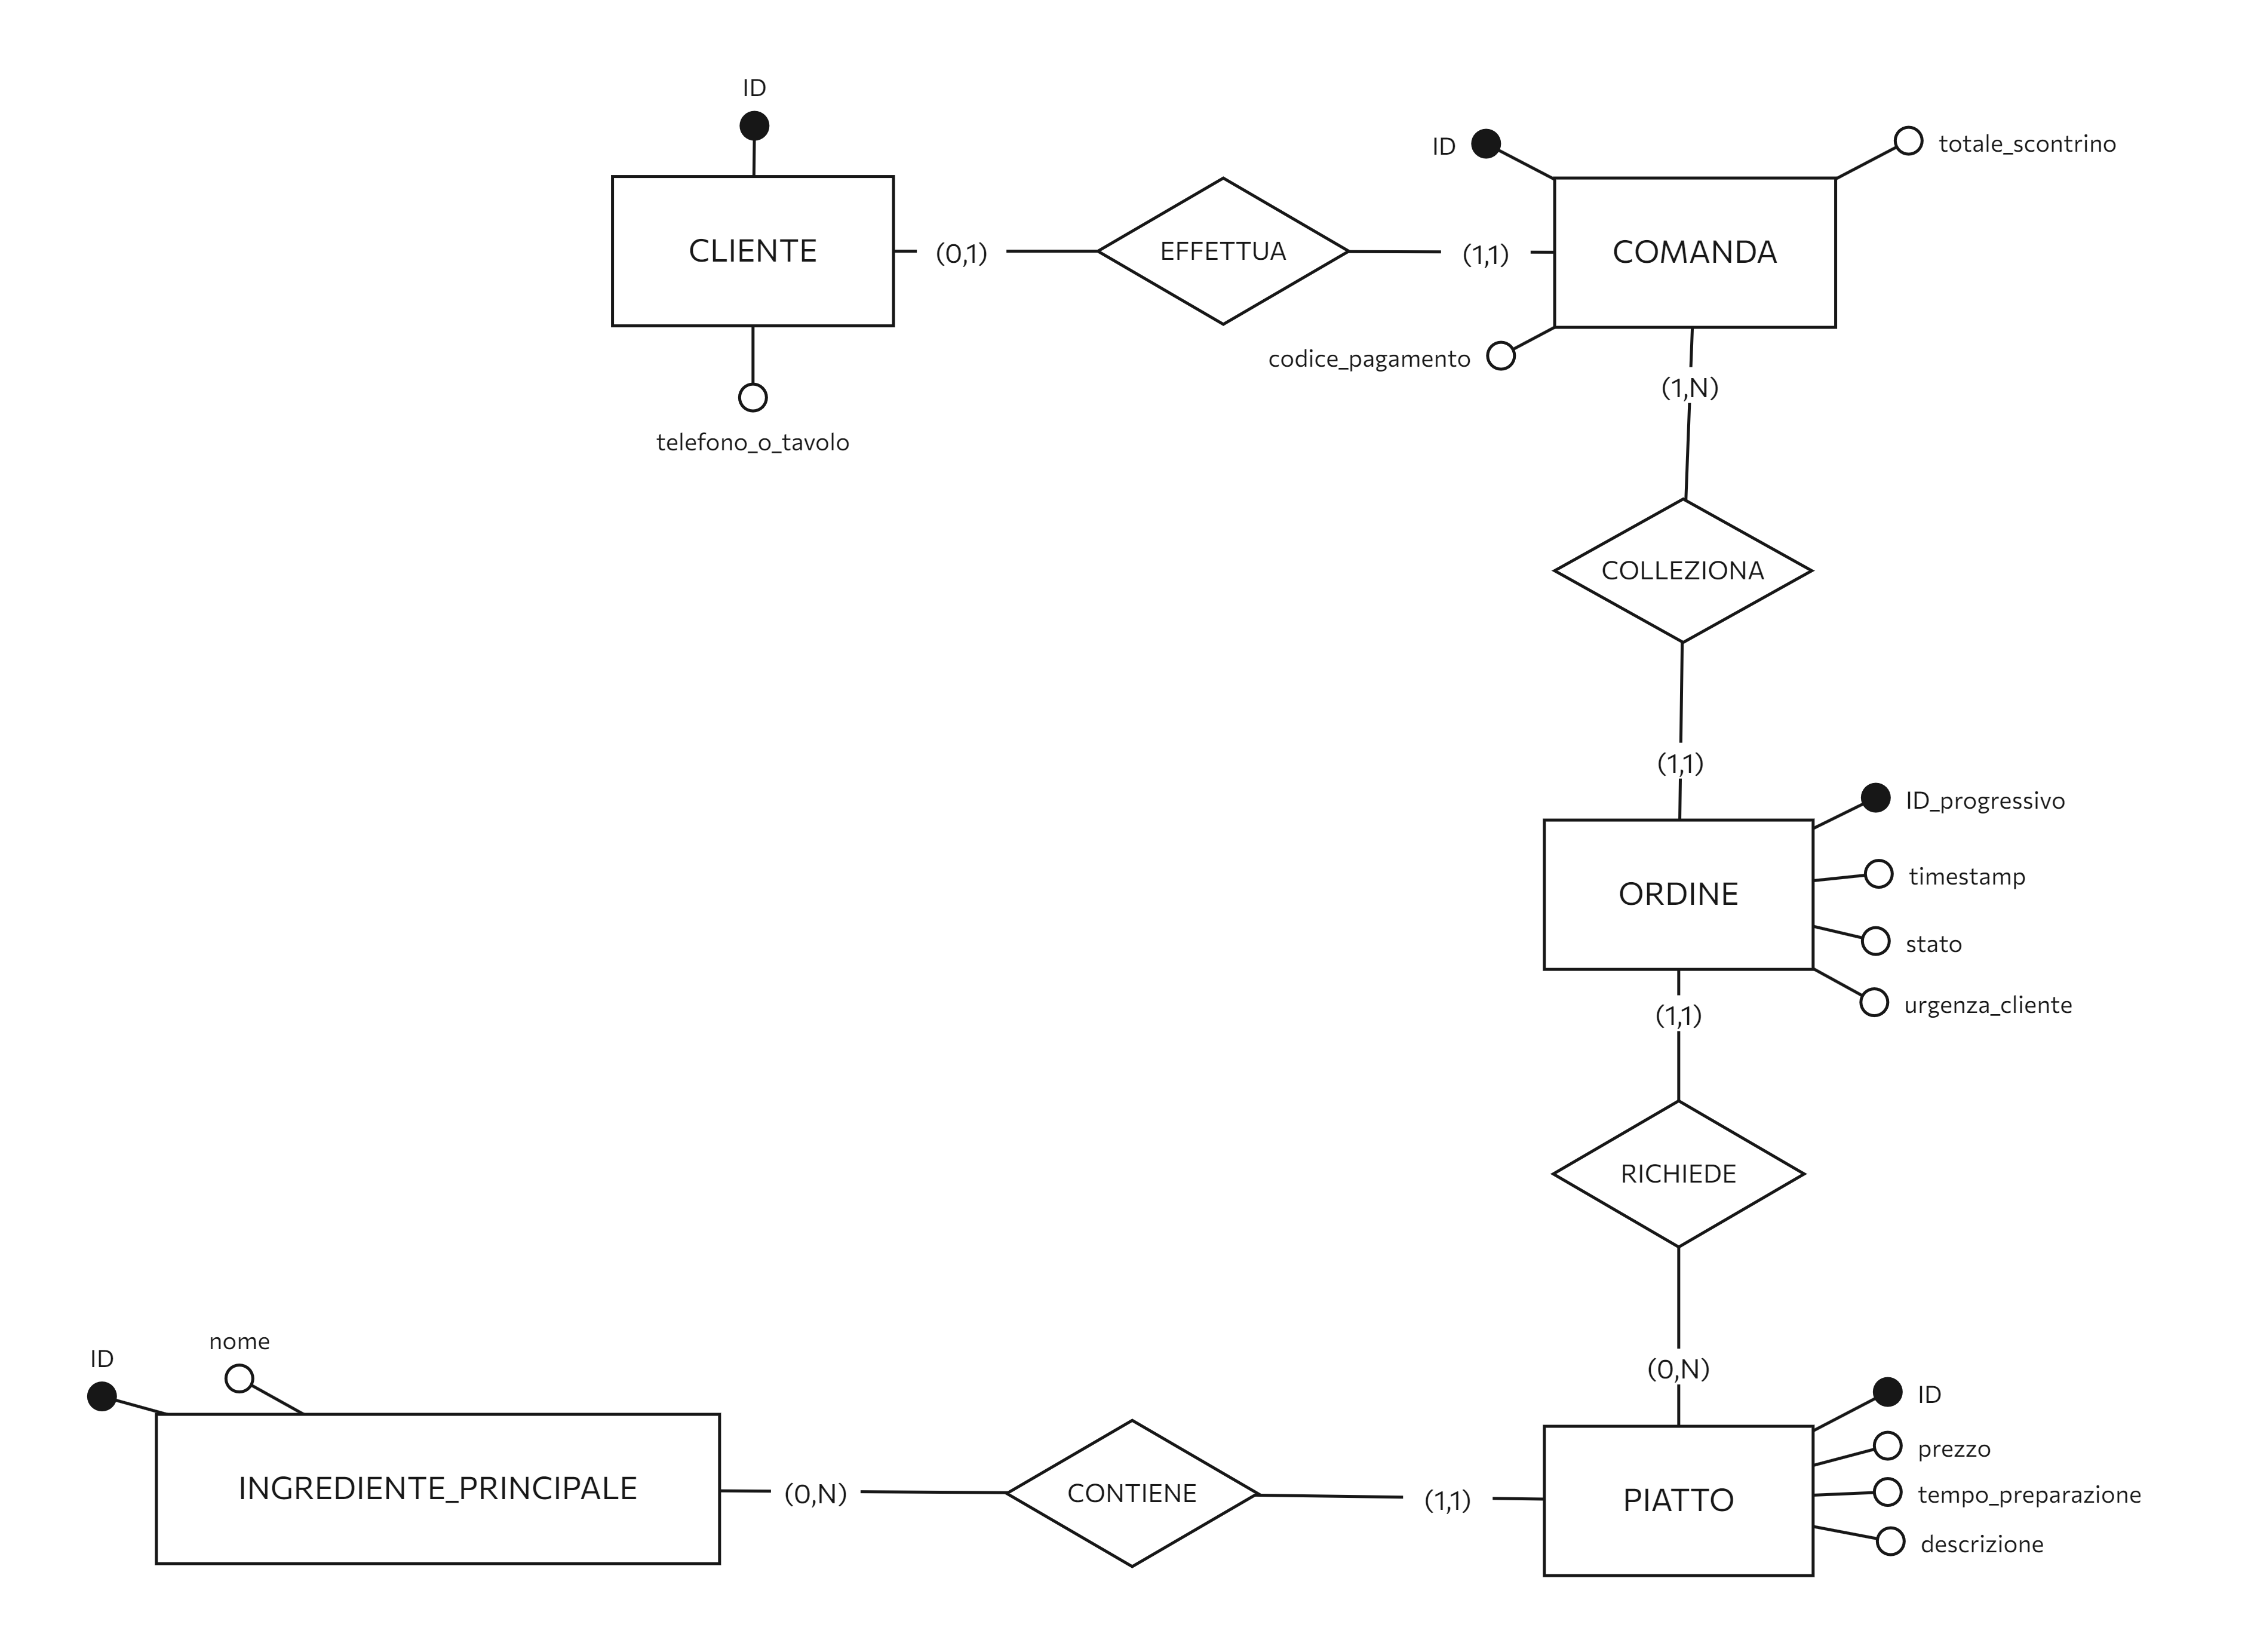
\includegraphics[scale=0.4]{iterazione1/images/ER_project_c.png}
	\caption{Modello Entità-relazione\label{fig:er_diagram}}
\end{figure}

\subsection{Modello logico}
Tramite il modello logico viene rappresentata in modo astratto la struttura dei dati così da facilitare la progettazione del database, definendo come i dati sono organizzati e come le entità interagiscono tra loro.
Rappresentazione della struttura dei dati all’interno del database. L’attributo di cliente::asporto\_o\_tavolo è stato pensato come un boolean in quanto il cliente può essere di due tipi:
\begin{itemize}
	\item se asporto\_o\_tavolo = 0, allora l’ID sarà il codice identificativo di un tavolo;
	\item se asporto\_o\_tavolo = 1, allora l’ID sarà un numero di telefono;
\end{itemize}

\begin{figure}[htbp]
	\centering
	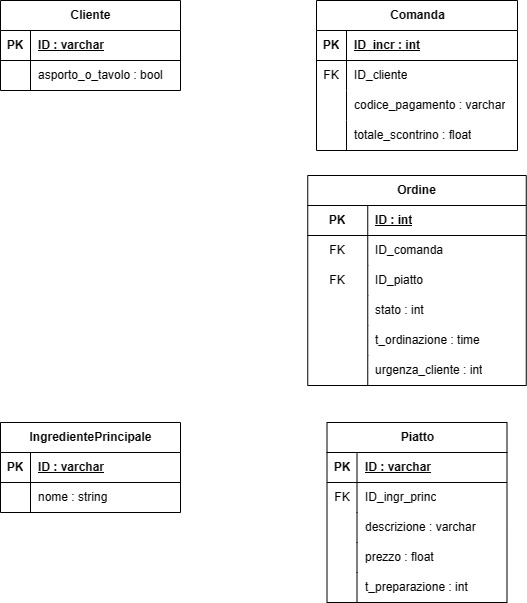
\includegraphics[scale=0.5]{iterazione1/images/database_modello_logico.jpg}
	\caption{Modello Logico\label{fig:modello_logico}}
\end{figure}

\newpage
Il modello logico è implementato con le seguenti query al database:

\begin{lstlisting}[language=SQL,caption=Query del database in SQL,label=lst:sqlcode]
	CREATE TABLE IF NOT EXISTS Cliente(
	ID varchar(10) PRIMARY KEY,
	t_o_a boolean NOT NULL
	);
	
	CREATE TABLE IF NOT EXISTS Comanda (
	ID int(10) AUTO_INCREMENT,
	ID_cliente varchar(10) NOT NULL,
	codice_pagamento varchar(255) DEFAULT NULL,
	totale_scontrino float DEFAULT 0.0,
	PRIMARY KEY (ID),
	FOREIGN KEY (ID_cliente) REFERENCES Cliente(ID)
	);
	
	CREATE TABLE IF NOT EXISTS IngredientePrincipale(
	ID varchar(20) PRIMARY KEY,
	nome varchar(20) NOT NULL
	);
	
	CREATE TABLE IF NOT EXISTS Piatto(
	ID varchar(20) NOT NULL PRIMARY KEY,
	ID_ingr_princ varchar(20) NOT NULL,
	descrizione varchar(50),
	prezzo float(6) NOT NULL,
	t_preparazione TIMESTAMP DEFAULT CURRENT_TIMESTAMP,
	FOREIGN KEY (ID_ingr_princ) REFERENCES IngredientePrincipale(ID)
	);
	
	CREATE TABLE IF NOT EXISTS Ordine(
	ID int(10) NOT NULL AUTO_INCREMENT,
	ID_comanda int(10) NOT NULL,
	ID_piatto varchar(20) NOT NULL,
	stato int(1) DEFAULT 0, -- 0=in preparazione, 1=completato
	t_ordinazione TIMESTAMP DEFAULT CURRENT_TIMESTAMP,
	urgenza_cliente int(2) DEFAULT 0, -- priorita' del cliente: 1=massima, -1=minima
	PRIMARY KEY (ID,ID_comanda),
	FOREIGN KEY (ID_comanda) REFERENCES Comanda(ID),
	FOREIGN KEY (ID_piatto) REFERENCES Piatto(ID),
	CHECK (stato >= 0 AND stato <=1 )
	);
\end{lstlisting}

\clearpage
    \section{Deployment Diagram}
Il diagramma mostra le istanze usate nella rete di container Docker adottata per creare l'applicazione e le loro relazioni. In particolare, si è scelto di implementare un'architettura event-driven con Kafka e Zookeeper su singolo host server.

\begin{figure}[htbp]
	\centering
	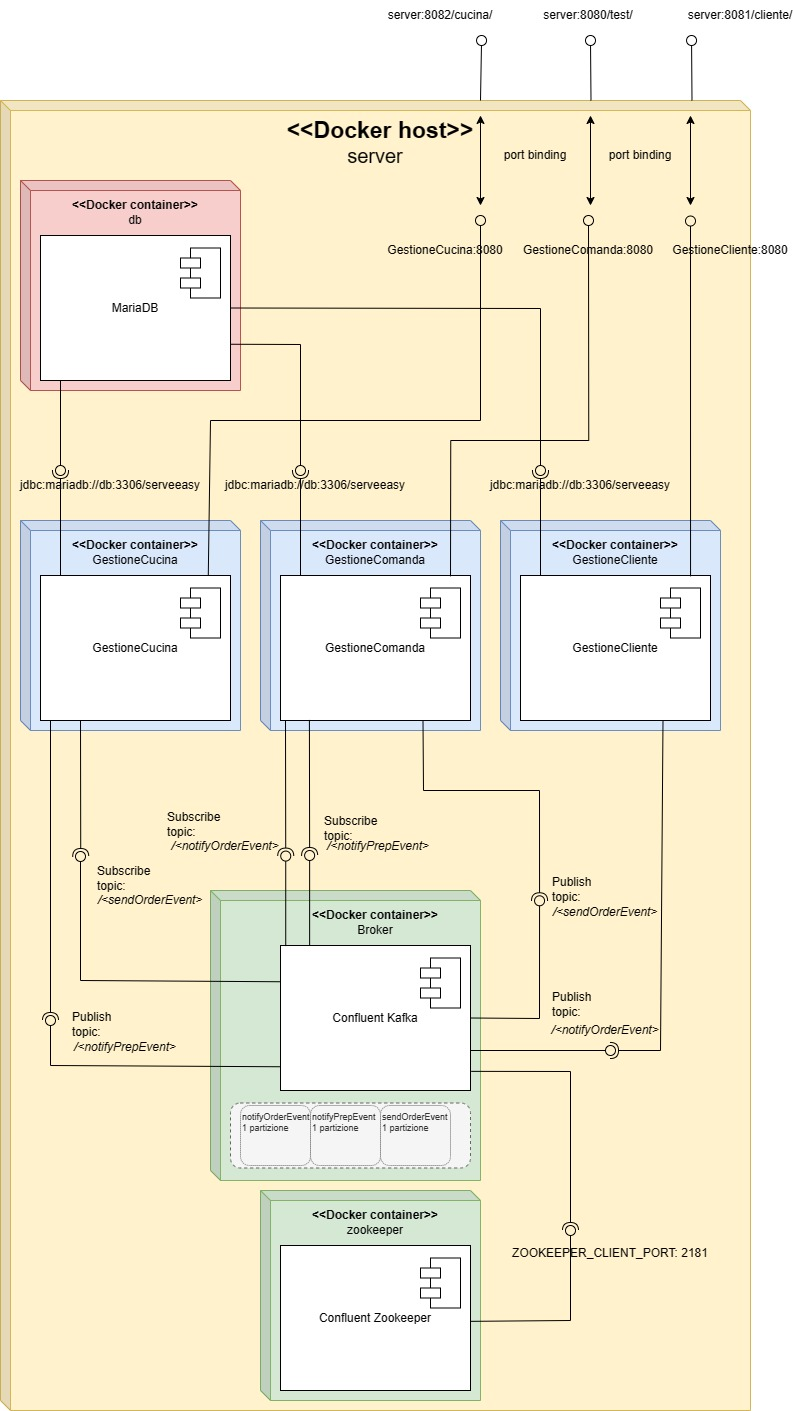
\includegraphics[scale=0.35]{iterazione1/images/deployment_iterazione1.jpg}
	\caption{Deployment Diagram
 \label{fig:deploymentdiagram}}
\end{figure}
\clearpage
    \section{Interface Class Diagram}
In questa sezione si definiscono in alto livello le interfacce, con relativi metodi, per la comunicazione tra i componenti e sottosistemi ottenuti. In particolare, vengono definiti con lo stereotipo \textbf{signal} i canali di comunicazione ad eventi, designati nel progetto per seguire un pattern publisher-subscriber.

\subsection{Interfacce Gestione Comanda}
\begin{figure}[H]
	\centering
	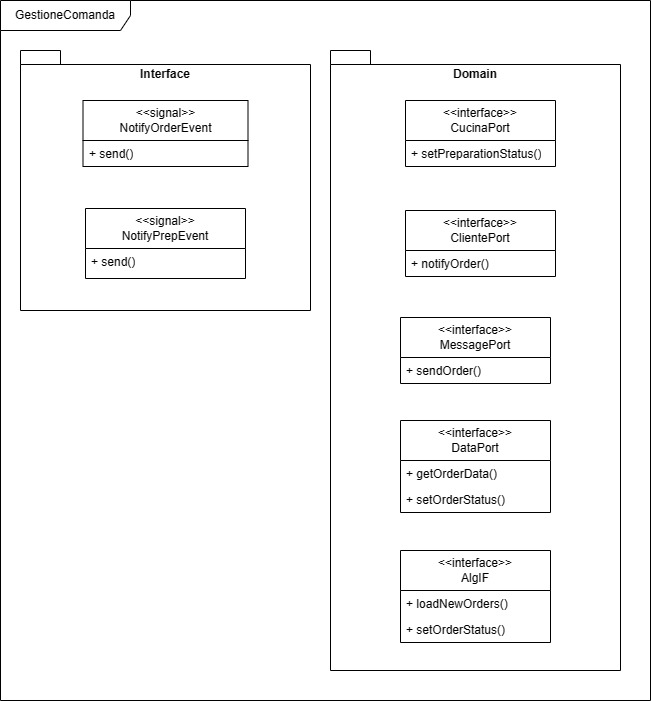
\includegraphics[scale=0.5]{iterazione1/images/GestioneComanda interface UML.jpg}
	\caption{Interface class diagram - Gestione Comanda\label{fig:interface_class_diagram_gestione_comanda}}
\end{figure}

\subsection{Interfacce Gestione Cucina}
\begin{figure}[H]
	\centering
	\includegraphics[scale=0.5]{iterazione1/images/GestioneCucina interface UML.jpg}
	\caption{Interface class diagram - Gestione Cucina\label{fig:interface_class_diagram_gestione_cucina}}
\end{figure}

\subsection{Interfacce Gestione Cliente}
\begin{figure}[H]
	\centering
	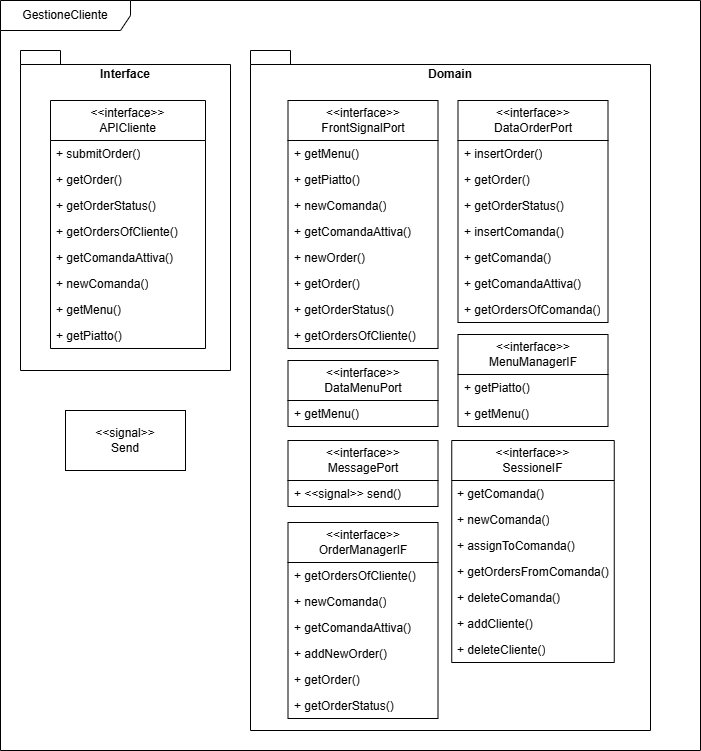
\includegraphics[scale=0.5]{iterazione1/images/GestioneCliente interface UML.jpg}
	\caption{Interface class diagram - Gestione Cliente\label{fig:interface_class_diagram_gestione_cliente}}
\end{figure}

\clearpage
    \section{Organizzazione del lavoro}

\subsection{Organizzazione del processo di sviluppo}
Per l’implementazione dei microservizi che compongono il sistema ServeEasy, attualmente delineato al primo zoom-in, è stato applicato un approccio “polyrepo"\cite{polyrepo}, definendo per ogni microservizio un’area di progetto dedicata. 

Scelta GitHub come piattaforma di hosting per il progetto software, un membro del team è stato incaricato del setup, controllo e gestione delle repository per i singoli microservizi.

Per raggiungere tale organizzazione, è stata prima di tutto creata un’area di lavoro per familiarizzare con le tecnologie selezionate, impiegando uno sforzo congiunto nello studio e prototipazione.

Nel processo di sviluppo sono state specificate delle regole mutualmente pattuite:
\begin{itemize}
    \item Nessuno esegue push diretto dall’area di lavoro locale verso il main branch: ognuno lavora esclusivamente sulla propria branch;
    \item Nei commit e nelle pull requests va espressa una sintesi del proprio lavoro svolto;
\item Cambiamenti importanti vanno discussi;
\item Ogni implementazione va testata;
\item Prima di effettuare una merge sul main branch, l’implementazione deve aver passato le fasi di build e di test con successo.
\end{itemize}

A supporto del processo di sviluppo, sono state introdotte automatizzazioni per garantire Continuous Integration e Continuous Delivery, servendosi di Github Workflows e Docker allo scopo di aumentare la velocità di deployment delle nuove modifiche apportate, garantendo al contempo integrità:
\begin{itemize}
    \item Un evento di push verso il proprio branch causa l’avvio della job di CI posta a sorveglianza del proprio spazio di lavoro sulla repository, allo scopo di effettuare un controllo di compilazione;
    \item Un evento verso il main branch (quale, ad esempio, una merge) causa l’avvio della job di CI/CD posta a sorveglianza del main sulla repository, la quale effettua un controllo di compilazione, genera un eseguibile e procede con le fasi di build e ship dell'immagine Docker corrispondente verso il registry DockerHub \cite{DockerOverview}.
\end{itemize}

In particolare, nel punto 2 si parla di Continuous Delivery e non Continuous Deployment, in quanto il deployment della nuova immagine va eseguita manualmente \cite{CDDocker}.

Il deployment verrà effettuato tramite Docker Compose: vengono definiti in un unico file i servizi offerti dal registry di riferimento (Dockerhub), le loro caratteristiche e dipendenze, cosicchè sarà sufficiente avviare il file per poter scaricare le immagini dei microservizi e servizi d’interesse in una rete di container dedicata.



\begin{figure}[htbp]
	\centering
	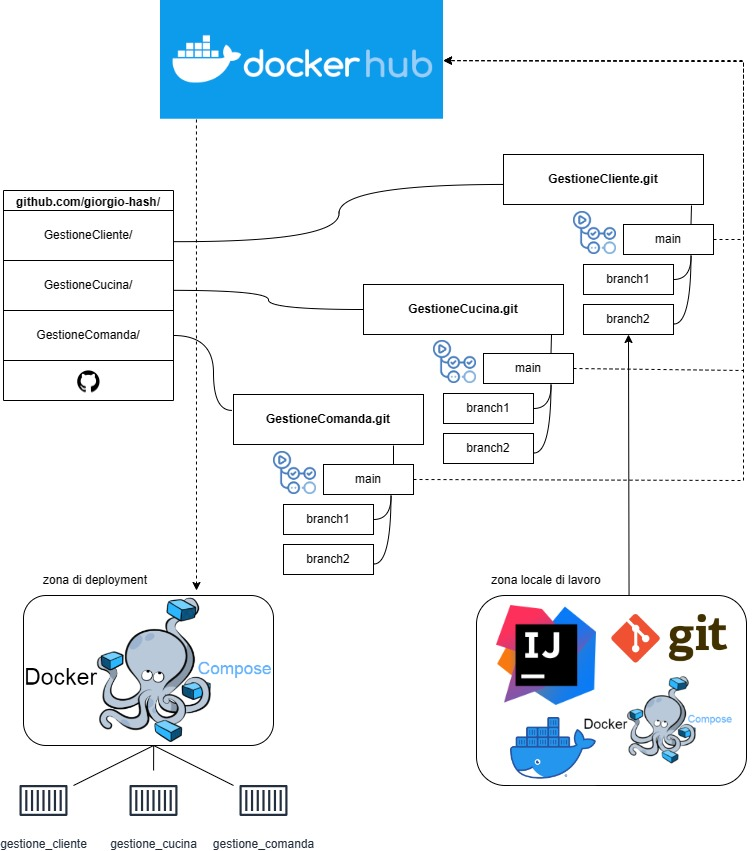
\includegraphics[scale=0.36]{iterazione1/images/DevOps.jpg}
	\caption{Organizzazione del lavoro cloud e locale, CI/CD e deployment 
 \label{fig:devopsit1}}
\end{figure}


\subsection{Organizzazione dell'area di lavoro}
Oltre all'IDE di Intellij IDEA e Git, l'area di lavoro locale è supportata da Docker Compose per attivare i servizi a supporto dell'esecuzione del singolo microservizio: non solo dipendenze, quali Kafka, Zookeeper ed il database MariaDB, ma anche strumenti utili per la visualizzazione ed interazione ad alto livello col sistema, quali:
\begin{itemize}
    \item Kafdrop per monitorare i messaggi passati tra pub e sub attraverso Kafka;
    \item PHPMyAdmin per monitorare, sviluppare ed iniettare dati nel database MariaDB.
\end{itemize}
Facendo leva sulla portabilità offerta dal framework Docker, viene garantito un ambiente altamente personalizzabile, flessibile e di facile implementazione. 

\begin{figure}[htbp]
	\centering
	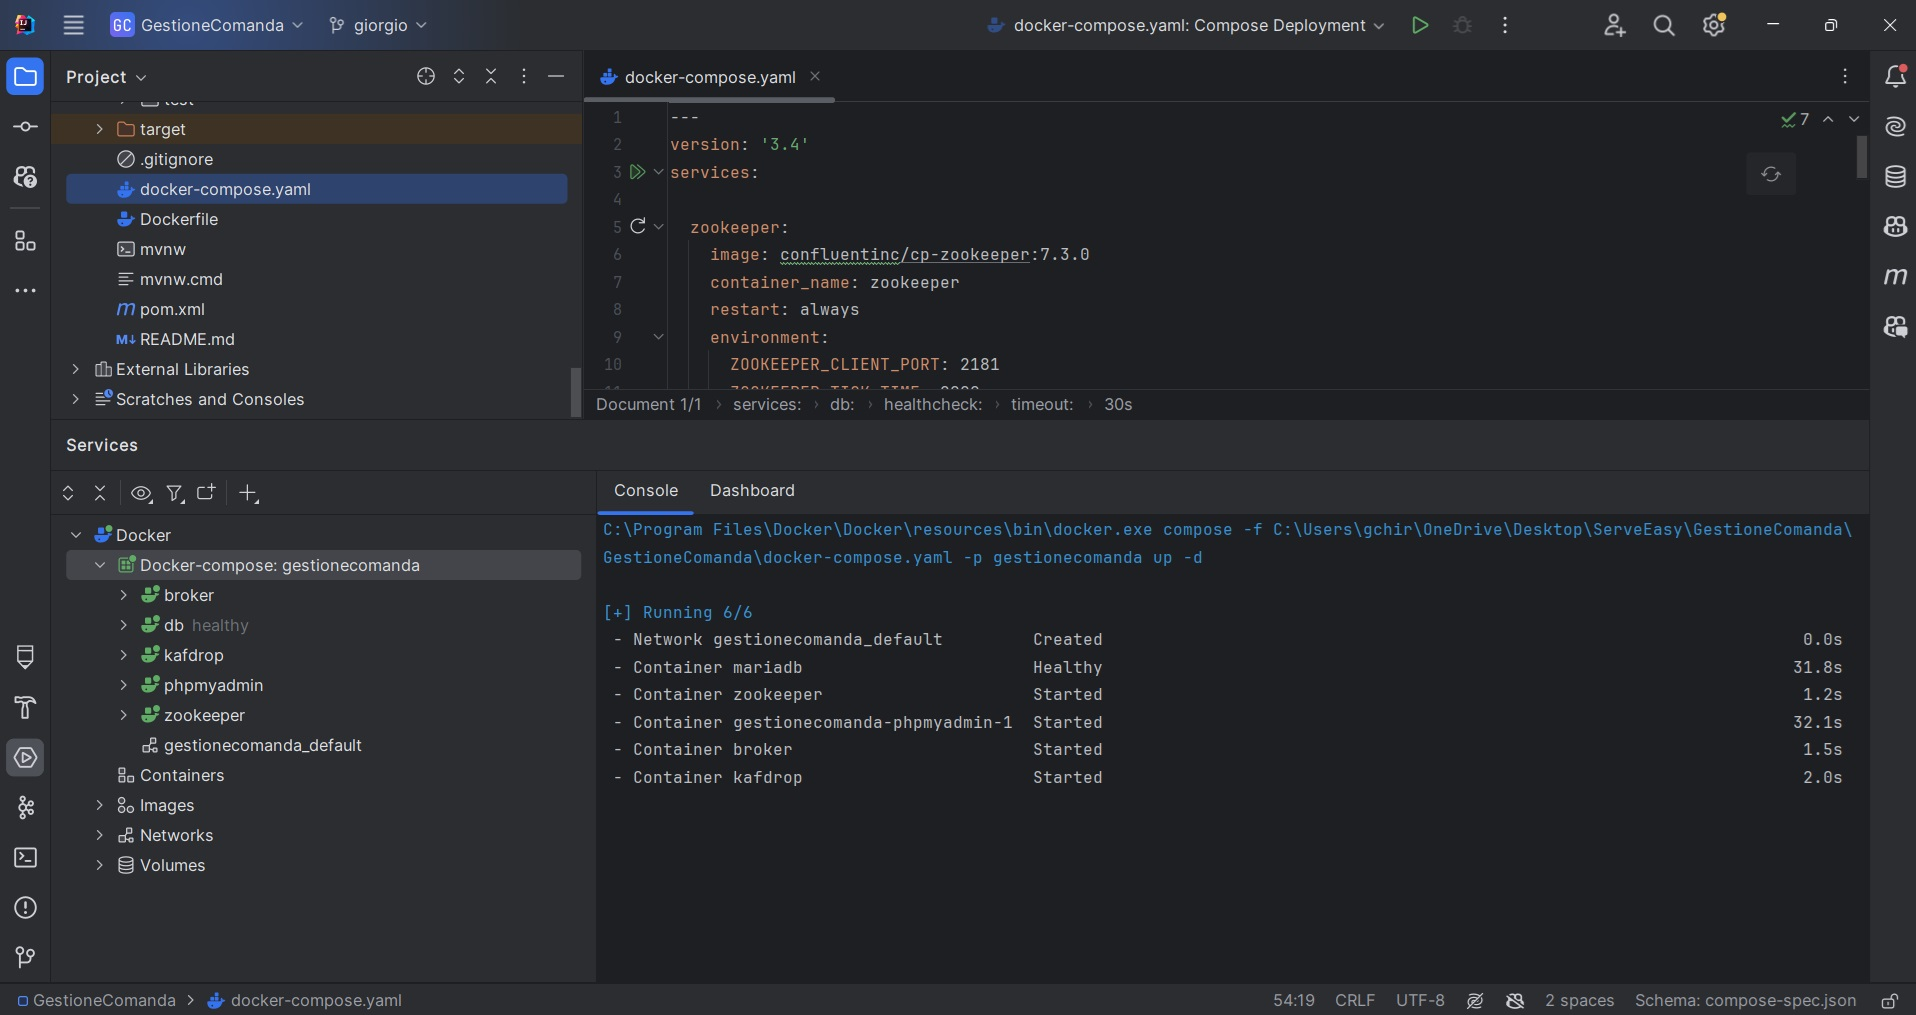
\includegraphics[scale=0.36]{iterazione1/images/IDEIDEA.jpg}
	\caption{Ambiente di lavoro con Intellij IDEA e Docker Compose
 \label{fig:IDEAit1}}
\end{figure}

Fin dal principio, l'area di lavoro è dotata della source tree che esplicita il layout dei subsystem identificati in fase di progettazione (paragrafo 2.3), comprendendo inoltre la cartella interfunzionale \textit{config}, necessaria per contenere gli artefatti di configurazione delle funzionalità (ad es. per JPA).

Alla radice del progetto, vi è inoltre una cartella dedicata a contenere dati di persistenza (cartella \textit{/db}).

\begin{figure}[htbp]
	\centering
	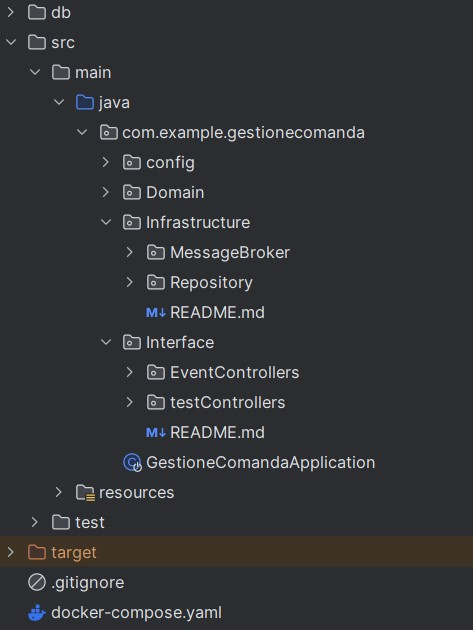
\includegraphics[scale=0.50]{iterazione1/images/source tree.jpg}
	\caption{source tree del progetto GestioneComanda
 \label{fig:srctreeGestioneComanda}}
\end{figure}

L'applicativo viene costruito per essere eseguito sulla macchina locale ed esposto su \textit{localhost:8080}. Lo sviluppo in locale è impostato per risolvere le dipendenze di rete dell'applicazione tramite il framework Docker: i servizi offerti da database e message broker vengono quindi eseguiti in container distinti nella rete \texttt{serveeasy\_default} creata da Docker (separata dalla rete \texttt{host} della macchina) ed esposte su \textit{localhost} attraverso la tecnica del port binding.

\begin{lstlisting}[language=yaml, caption={port-binding del servizio \textit{broker} alla voce \textit{ports} (porta\_host:porta\_container) }, label=lst:port-binding]
[...]
	|\color{codeMediumDarkblue}broker|:
		|\color{codeMediumDarkblue}image|: confluentinc/|\color{black}cp-kafka:7.3.0|
		|\color{codeMediumDarkblue}container\_name|: broker
		|\color{codeMediumDarkblue}restart|: always
		|\color{codeMediumDarkblue}ports|:
		- "9092:9092"
[...]
\end{lstlisting}

\clearpage
    \section{Costruzione dello scheletro}

\subsection{Organizzazione del processo di sviluppo}
Per l’implementazione dei microservizi che compongono il sistema ServeEasy, attualmente delineato al primo zoom-in, è stato applicato un approccio “polyrepo"\cite{polyrepo}, definendo per ogni microservizio un’area di progetto dedicata. 

Scelta GitHub come piattaforma di hosting per il progetto software, un membro del team è stato incaricato del setup, controllo e gestione delle repository per i singoli microservizi.

Per raggiungere tale organizzazione, è stata prima di tutto creata un’area di lavoro per familiarizzare con le tecnologie selezionate, impiegando uno sforzo congiunto nello studio e prototipazione.

Nel processo di sviluppo sono state specificate delle regole mutualmente pattuite:
\begin{itemize}
    \item Nessuno esegue push diretto dall’area di lavoro locale verso il main branch: ognuno lavora esclusivamente sulla propria branch;
    \item Nei commit e nelle pull requests va espressa una sintesi del proprio lavoro svolto;
\item Cambiamenti importanti vanno discussi;
\item Ogni implementazione va testata;
\item Prima di effettuare una merge sul main branch, l’implementazione deve aver passato le fasi di build e di test con successo.
\end{itemize}

A supporto del processo di sviluppo, sono state introdotte automatizzazioni per garantire Continuous Integration e Continuous Delivery, servendosi di Github Workflows e Docker allo scopo di aumentare la velocità di deployment delle nuove modifiche apportate, garantendo al contempo integrità:
\begin{itemize}
    \item Un evento di push verso il proprio branch causa l’avvio della job di CI posta a sorveglianza del proprio spazio di lavoro sulla repository, allo scopo di effettuare un controllo di compilazione;
    \item Un evento verso il main branch (quale, ad esempio, una merge) causa l’avvio della job di CI/CD posta a sorveglianza del main sulla repository, la quale effettua un controllo di compilazione, genera un eseguibile e procede con le fasi di build e ship dell'immagine Docker corrispondente verso il registry DockerHub \cite{DockerOverview}.
\end{itemize}

In particolare, nel punto 2 si parla di Continuous Delivery e non Continuous Deployment, in quanto il deployment della nuova immagine va eseguita manualmente \cite{CDDocker}.

Il deployment verrà effettuato tramite Docker Compose: vengono definiti in un unico file i servizi offerti dal registry di riferimento (Dockerhub), le loro caratteristiche e dipendenze, cosicchè sarà sufficiente avviare il file per poter scaricare le immagini dei microservizi e servizi d’interesse in una rete di container dedicata.



\begin{figure}[htbp]
	\centering
	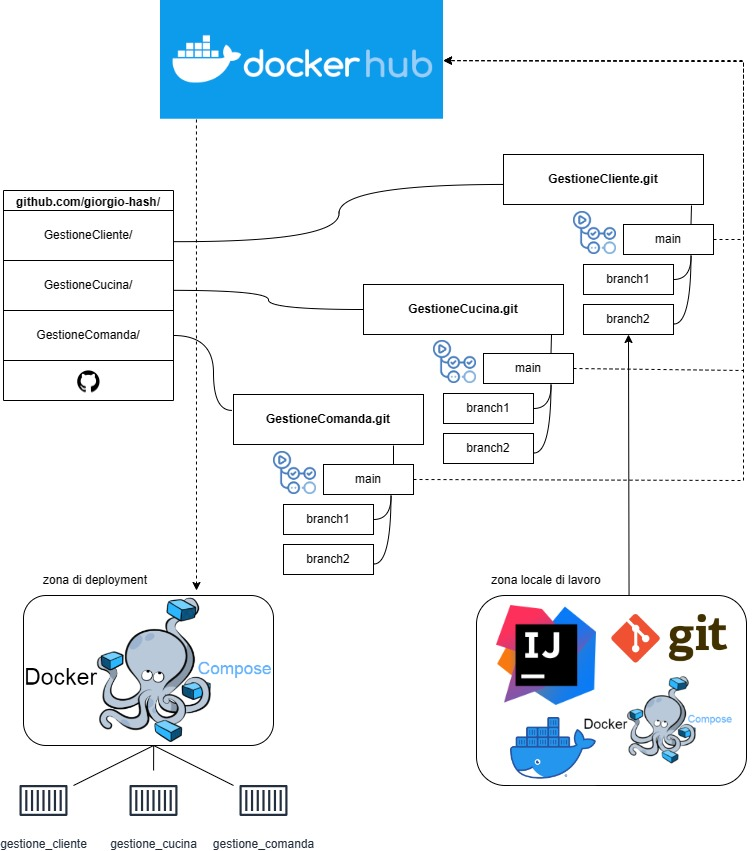
\includegraphics[scale=0.36]{iterazione1/images/DevOps.jpg}
	\caption{Organizzazione del lavoro cloud e locale, CI/CD e deployment 
 \label{fig:devopsit1}}
\end{figure}


\subsection{Organizzazione dell'area di lavoro}
Oltre all'IDE di Intellij IDEA e Git, l'area di lavoro locale è supportata da Docker Compose per attivare i servizi a supporto dell'esecuzione del singolo microservizio: non solo dipendenze, quali Kafka, Zookeeper ed il database MariaDB, ma anche strumenti utili per la visualizzazione ed interazione ad alto livello col sistema, quali:
\begin{itemize}
    \item Kafdrop per monitorare i messaggi passati tra pub e sub attraverso Kafka;
    \item PHPMyAdmin per monitorare, sviluppare ed iniettare dati nel database MariaDB.
\end{itemize}
Facendo leva sulla portabilità offerta dall'ambiente Docker, viene garantito un ambiente altamente personalizzabile, flessibile e di facile implementazione. 



\subsection{Definizione Interfacce}
% nota: metterei solo quelle di gestione comanda oppure quelle che ci servono per spiegare
\begin{lstlisting}[style=myJava, 
    caption={Interfaccia MessagePort}, label=lst:messageport,]
public interface MessagePort<T> {
    /**
     * Invia l'oggetto passato come parametro sul topic del message broker
     *
     * @param t oggetto da inviare
     * @throws JsonProcessingException eccezione sollevata nella serializzazione
     */
    void send(T t) throws JsonProcessingException;
}
\end{lstlisting}

\begin{lstlisting}[style=myJava, 
    caption={Interfaccia DataPort}, label=lst:dataport]
public interface DataPort {

    /**
     * Controlla se l'ordine esiste nel database
     *
     * @param id id dell'entita' ordine da controllare la presenza
     * @return true se esiste, false altrimenti
     */
    boolean isOrderExist(int id);

    /**
     * Salva l'entita' ordine all'interno del database
     *
     * @param ordineEntity entita' ordine da salvare
     * @return entita' ordine salvata
     */
    OrdineEntity saveOrder(OrdineEntity ordineEntity);

    /**
     * Cerca nel db e restituisce l'ordine corrispondente all' id dato
     *
     * @param id id dell'ordine
     * @return Optional(OrdineEntity) se esiste altrimenti Optional(null)
     */
    Optional<OrdineEntity> getOrderById(int id);

    /**
     * Aggiorna l'attributo stato dell'ordine
     *
     * @param id id dell'ordine su cui effetturare l'aggiornamento
     * @param ordineEntity entita' con gli aggiornamenti parziali da applicare
     * @return entita' aggiornata
     */
    OrdineEntity updateOrder(int id, OrdineEntity ordineEntity);


    /**
     * Lista di tutti gli ordini per una specifica comanda
     *
     * @param idComanda id della comanda su cui cercare gli ordini
     * @return lista di ordini per una data comanda
     */
    List<OrdineEntity> findAllOrdersByIdComanda(int idComanda);

    /**
     * Cancella l'ordine con il dato ID dal databse
     *
     * @param id id dell'ordine da eliminare
     */
    void deleteOrder(int id);
}
\end{lstlisting}

\begin{lstlisting}[style=myJava, 
    caption={Interfaccia NotifyOrderEvent}, label=lst:notifyordereventIF,]
public interface NotifyOrderEvent {

    /**
     * Riceve un messaggio tramite Kafka dal servizio gestioneCliente in merito all'avvenuta ordinazione
     * da parte di un cliente
     *
     * @param message il corpo del messaggio vero e proprio
     * @param topic topic del message broker sul quale si riceve il messaggio
     * @param partition numero di partizione sul quale si riceve il messaggio
     * @param offset numero di offset che presenta il messaggio ricevuto
     */
    @KafkaListener(id = "${spring.kafka.consumer.gestioneCliente.group-id}", topics = "${spring.kafka.consumer.gestioneCliente.topic}")
    void receive(String message, String topic, Integer partition, Long offset) throws JsonProcessingException;

    /**
     * Restituisce l'ultima notifica letta dal listener
     *
     * @return oggetto notifica letto dal listener
     */
    NotificaOrdineDTO getLastMessageReceived();
}
\end{lstlisting}

%TODO: ho aggiunto solo quelle che mi servono per poter avere il riferimento

\subsection{Adattatore Kafka}
Lo sviluppo del componente adibito all'adattatore Kafa è stato un processo che ha seguito vari step:
\paragraph{Step 1 - Overview:}
Come primo passo ci si è fatti una panoramica leggendo la documentazione ufficiale di Spring Kafka \cite{SpringKafka} e si sono cercati alcuni progetti su Github di \href{https://github.com/devtiro/spring-boot-kafka-tutorial/tree/main}{esempio}.
\paragraph{Step 2 - Setup:}
Al passo numero due ci si è focalizzati sul setup dell’ambiente di lavoro, si sono definiti i seguenti container nel file "docker-compose.yaml" (Codice \vref{lst:docker-compose1}):
\begin{lstlisting}[language=docker-compose, caption={Setup del docker-compose.yaml per l'adattatore Kafka}, label=lst:docker-compose1]
services:  
  zookeeper:
    image: confluentinc/cp-zookeeper:7.3.0
    container_name: zookeeper
    restart: always
    environment:
      ZOOKEEPER_CLIENT_PORT: 2181
      ZOOKEEPER_TICK_TIME: 2000

  broker:
    image: confluentinc/cp-kafka:7.3.0
    container_name: broker
    restart: always
    ports:
      - "9092:9092"
    depends_on:
      - zookeeper
    environment:
      KAFKA_BROKER_ID: 1
      KAFKA_ZOOKEEPER_CONNECT: 'zookeeper:2181'
      KAFKA_LISTENER_SECURITY_PROTOCOL_MAP: PLAINTEXT:PLAINTEXT,PLAINTEXT_INTERNAL:PLAINTEXT
      KAFKA_ADVERTISED_LISTENERS: PLAINTEXT://localhost:9092,PLAINTEXT_INTERNAL://broker:29092
      KAFKA_OFFSETS_TOPIC_REPLICATION_FACTOR: 1
      KAFKA_TRANSACTION_STATE_LOG_MIN_ISR: 1
      KAFKA_TRANSACTION_STATE_LOG_REPLICATION_FACTOR: 1
\end{lstlisting}
Fatto ciò si è passati ad aggiornare il file "pom.xml" (Codice \vref{lst:pom-xml1}) con la seguente dipendenza per Kafka: 
\begin{lstlisting}[language=XML, caption={Aggiornamento dipendenze nel pom.xml per includere spring-kafka}, label=lst:pom-xml1]
<dependency>
    <groupId>org.springframework.kafka</groupId>
    <artifactId>spring-kafka</artifactId>
</dependency>
\end{lstlisting}
Successivamente nel file "application.yml" (Codice \vref{lst:application-yml1}) sono state aggiunte le seguenti istruzioni di configurazione, come si può notare si è partiti inizialmente solamente a considerare un'applicazione costituita da un singolo producer senza consumer:
\begin{lstlisting}[language=yaml, caption={Aggiornamento del file `application.yml` per il producer Kafka}, label=lst:application-yml1]
spring:
  kafka:
    bootstrap-servers: localhost:9092
    producer:
      topic: sendOrderEvent
      group-id: gestioneComanda
\end{lstlisting}
Sono stati poi creati i primi bean di configurazione nella classe "KafkaConfig.java" (Codice \vref{lst:KafkaConfig}):
\begin{lstlisting}[style=myJava, 
    caption={Classe di configurazione KafkaConfig.java}, label=lst:KafkaConfig, 
    emph={[2] BOOTSTRAP_SERVERS_CONFIG, KEY_SERIALIZER_CLASS_CONFIG ,  VALUE_SERIALIZER_CLASS_CONFIG, bootstrapServers },
    emphstyle={[2]\color{codeDarkMagenta}},]
@Configuration
public class KafkaConfig {

    @Value("${spring.kafka.bootstrap-servers}")
    private String bootstrapServers;

    @Bean
    public ProducerFactory<String, String> producerFactory() {
        Map<String, Object> configProps = new HashMap<>();
        configProps.put(ProducerConfig.BOOTSTRAP_SERVERS_CONFIG, bootstrapServers);
        configProps.put(ProducerConfig.KEY_SERIALIZER_CLASS_CONFIG, StringSerializer.class);
        configProps.put(ProducerConfig.VALUE_SERIALIZER_CLASS_CONFIG, StringSerializer.class);
        return new DefaultKafkaProducerFactory<>(configProps);
    }

    @Bean
    public KafkaTemplate<String, String> kafkaTemplate() {
        return new KafkaTemplate<>(producerFactory());
    }
}
\end{lstlisting}
E di Object Mapper (Codice \vref{lst:jsonconfig}) per la serializzazione e deserializzazione in formato JSON, visto che la comunicazione tramite message broker avviene tramite messaggi in quel formato:
\begin{lstlisting}[style=myJava, 
    caption={Classe di configurazione JsonConfig.java}, label=lst:jsonconfig,]
@Configuration
public class JsonConfig {

    @Bean
    public ObjectMapper objectMapper(){
        final ObjectMapper objectMapper = new ObjectMapper();
        // configurazione di timestamp
        objectMapper.registerModule(new JavaTimeModule());
        objectMapper.setDateFormat(new SimpleDateFormat("yyyy-MM-dd HH:mm:ss.SSS"));
        return objectMapper;
    }
}
\end{lstlisting}
\paragraph{Step 3 - Producer:}
Nel passo successivo si è passati a creare la prima classe adibita al compito di producer kafka, ossia CucinaPubProducer.java (Codice \vref{lst:CucinaPubProducer}) che implementa la MessagePort (Codice \vref{lst:messageport}):
\begin{lstlisting}[style=myJava, 
    caption={Classe del producer kafka CucinaPubProducer.java}, label=lst:CucinaPubProducer, 
    emph={[2] kafkaTemplate , objectMapper, topic, payload, log },
    emphstyle={[2]\color{codeDarkMagenta}}]
@Service
@Log
public class CucinaPubProducer implements MessagePort<OrdineDTO> {

    private final KafkaTemplate<String, String> kafkaTemplate;

    private final ObjectMapper objectMapper;

    /**
     * topic sul quale e' in ascolto la cucina
     */
    @Value("${spring.kafka.producer.topic}")
    private String topic;

    @Autowired
    public CucinaPubProducer(final KafkaTemplate<String, String> kafkaTemplate, final ObjectMapper objectMapper){
        this.kafkaTemplate = kafkaTemplate;
        this.objectMapper = objectMapper;
    }

    @Override
    public void send(OrdineDTO ordineDTO) throws JsonProcessingException {

        // Serializza in un oggetto JSON
        final String payload = objectMapper.writeValueAsString(ordineDTO);

        // invia messaggio sul topic specificato
        CompletableFuture<SendResult<String, String>> future = kafkaTemplate.send(topic, payload);
        future.whenComplete((result,ex)->{
            if(ex == null){
                log.info("Sent Message=[" + payload + "] with offset=[" + result.getRecordMetadata().offset() + "]");
            }
            else{
                log.info("Unable to send message=[" + payload + "] due to : " + ex.getMessage());
            }
        });
    }
}
\end{lstlisting}
Si può notare che questa classe richiede un bean di ObjectMapper (Codice \vref{lst:jsonconfig}) e KafkaTemplate (Codice \vref{lst:KafkaConfig}) definiti al passo precedente, mentre richiede dall’application.yml (Codice \vref{lst:application-yml1}) il nome del topic kafka in questione.
Inizialmente si è usato una stringa “Hello world” al posto dell’oggetto OrdineDTO e si è verificato il funzionamento tramite log sulla console, per poter iniettare messaggi si è utilizzata l’istruzione tramite terminale:
\begin{lstlisting}[style=terminal, 
    caption={Operazione di post sul topic kafka}, label=lst:postkafka]
docker exec --interactive --tty broker kafka-console-producer --bootstrap-server broker:9092 --topic "sendOrderEvent"
\end{lstlisting}
mentre per ricevere messaggi:
\begin{lstlisting}[style=terminal, 
    caption={Operazione di get sul topic kafka}, label=lst:getkafka]
docker exec --interactive --tty broker kafka-console-consumer --bootstrap-server broker:9092 --topic "notifyOrderEvent" --from-beginning
\end{lstlisting}
\paragraph{Step 4 - User Interface} 
Verificato il funzionamente tramite log si è passati ad usare Kafdrop\cite{kafdrop} ossia una User Interface (UI) per i topic di Kafka, integrandolo nella nostra applicazione con le seguenti istruzioni nel docker-compose.yml:(Codice \vref{lst:docker-compose2}):
\begin{lstlisting}[language=docker-compose, caption={Aggiornamento del docker-compose.yaml perl per Kafdrop}, label=lst:docker-compose2]
services:  
  kafdrop:
    image: obsidiandynamics/kafdrop
    container_name: kafdrop
    restart: "no"
    ports:
      - "9000:9000"
    environment:
      KAFKA_BROKERCONNECT: "broker:29092"
    depends_on:
      - "broker"
\end{lstlisting}
Di seguito (Figura \vref{fig:kafdrop_funzionamento}) viene mostrato un esempio della UI in funzione sulla porta localhost:9000 che mostra tutti i messaggi postati sul topic \textit{sendOrderEvent} ordinati in base all'offset:
\begin{figure}[H]
    \centering
    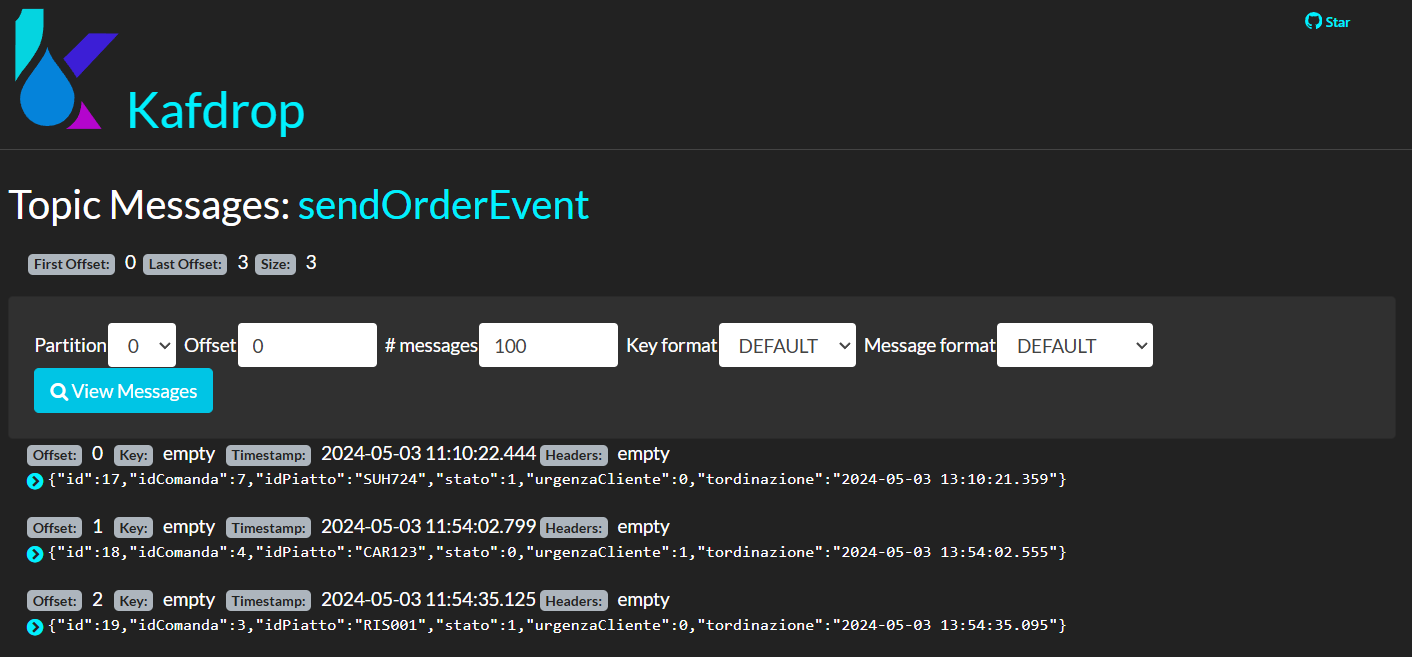
\includegraphics[width=1\linewidth]{iterazione1//images/kafdrop_esempio_funzionamento.png}
    \caption{Esempio funzionamento kafdrop}
    \label{fig:kafdrop_funzionamento}
\end{figure}
\paragraph{Step 5 - Testing}
In questo passo è stato creato il primo test di integrazione per il producer per verificare il corretto invio di un messaggio sul topic tramite il producer appena creato e la ricezione tramite un consumer simulato utilizzando un'istanza Embedded Kafka \cite{TestingKafka}.
Embedded Kafka è una libreria che fornisce istanze di Kafka e Confluent Schema Registry in memoria per eseguire i test, in modo da non dipendere da un server Kafka esterno.
Viene quindi integrata nel pom.xml (Codice \vref{lst:pom-xml2}) la seguente dipendenza:
\begin{lstlisting}[language=XML, caption={Aggiornamento dipendenze nel pom.xml per includere spring-kafka-test}, label=lst:pom-xml2]
<dependency>
    <groupId>org.springframework.kafka</groupId>
    <artifactId>spring-kafka-test</artifactId>
    <scope>test</scope>
</dependency>
\end{lstlisting}
E aggiornato l’application.properties specifico dei test  (Codice \vref{lst:application-properties1}):
\begin{lstlisting}[language=yaml, caption={Aggiornamento del file `application.properties` di test per il producer kafka}, label=lst:application-properties1]
spring.kafka.bootstrap-servers=localhost:9092
spring.kafka.consumer.auto-offset-reset= earliest
spring.kafka.producer.topic=test.topic.comanda
\end{lstlisting}
Fatto ciò si può procedere a scrivere la seguente classe di test (Codice \vref{lst:CucinaPubProducerTest}):
\begin{lstlisting}[style=myJava, 
    caption={Test di integrazione per il producer CucinaPubProducer}, label=lst:CucinaPubProducerTest, 
    emph={[2] kafkaTemplate , objectMapper, topic, payload, log, producer, embeddedKafka, logger, testAppender },
    emphstyle={[2]\color{codeDarkMagenta}}]
@EnableKafka
@SpringBootTest()
@DirtiesContext
@TestMethodOrder(MethodOrderer.OrderAnnotation.class)
@EmbeddedKafka(partitions = 1,
        controlledShutdown = false,
        brokerProperties = { "listeners=PLAINTEXT://localhost:9092", "port=9092" },
        topics = {"${spring.kafka.producer.topic}"})
class CucinaPubProducerTests {

    @Autowired
    private CucinaPubProducer producer;
    @Autowired
    private EmbeddedKafkaBroker embeddedKafka;
    @Autowired
    private ObjectMapper objectMapper;
    @Value("${spring.kafka.producer.topic}")
    private String topic;
    private Logger logger;
    private TestAppender testAppender;

    @BeforeEach
    public void setup() {
        logger = (Logger) LoggerFactory.getLogger(CucinaPubProducer.class);
        testAppender = new TestAppender();
        testAppender.start();
        logger.addAppender(testAppender);
    }

    @Test
    public void testSendingMessage() throws JsonProcessingException {

        OrdineDTO ordineDTO = TestDataUtil.createOrdineDtoA();

        producer.send(ordineDTO);
        String message = objectMapper.writeValueAsString(ordineDTO);

        // configurazione del consumer di Embedded Kafka
        Map<String, Object> consumerProps = KafkaTestUtils.consumerProps("testT", "false", embeddedKafka);
        DefaultKafkaConsumerFactory<Integer, String> cf = new DefaultKafkaConsumerFactory<>(consumerProps);
        Consumer<Integer, String> consumer = cf.createConsumer();
        embeddedKafka.consumeFromAnEmbeddedTopic(consumer, topic);
        ConsumerRecord<Integer, String> received = KafkaTestUtils.getSingleRecord(consumer, topic);

        // testo il corretto invio
        assertFalse(testAppender.events.isEmpty());
        assertEquals("Sent Message=[" + message + "] with offset=[0]", testAppender.events.get(0).getFormattedMessage());

        // testo la corretta ricezione
        assertThat(received.offset()).isEqualTo(0);
        assertThat(received.topic()).isEqualTo(topic);
        assertThat(received.partition()).isEqualTo(0);
        OrdineDTO ordineDTOReceived = objectMapper.readValue(received.value(),OrdineDTO.class);
        assertThat(ordineDTOReceived).isEqualTo(ordineDTO);

        logger.detachAppender(testAppender);
    }
}
\end{lstlisting}
Che testa il corretto invio di un oggetto creato tramite la classe di supporto testDataUtil e verifica inizialmente che il log della classe CucinaPubAdapter sia quello che ci si aspetta, mentre successivamente verifica che il consumer creato utilizzando un’istanza di EmbeddedKafka riceva l’oggetto inviato, viene di conseguenza testata anche la serializzazione.
\paragraph{Step 6 - Consumer}
Creato e testato il producer si è passati alla creazione di un consumer, inizialmente si è creato un consumer generico in ascolto sullo stesso topic del producer appena creato, verificato il funzionamento si è passati a creare i due producer richiesti in maniera speculare, di seguito verrà mostrato il producer in ascolto sul topic del microservizio di Gestione Cliente ossia SubClienteAdapter.
Come prima cosa si è aggiornato l’application.yml (Codice \vref{lst:application-yml2}) con la configurazione del consumer in questione:
\begin{lstlisting}[language=yaml, caption={Aggiornamento del file `application.yml` per il consumer Kafka}, label=lst:application-yml2]
kafka:
 consumer:
   gestioneCliente:
     topic: notifyOrderEvent
     group-id: gestioneCliente
\end{lstlisting}
Poi si è passati direttamente ad implementare la classe SubClienteAdapter (Codice: \vref{lst:subclienteadapter})  che implementa l'interfaccia NotifyOrderEvent (Codice: \vref{lst:notifyordereventIF})  
\begin{lstlisting}[style=myJava, 
    caption={Classe del consumer kafka SubClienteAdapter.java}, label=lst:subclienteadapter, 
    emph={[2] kafkaTemplate , objectMapper, topic, payload, log, producer, embeddedKafka, logger, testAppender, RECEIVED_TOPIC, RECEIVED_PARTITION, OFFSET, clientePort, lastMessageReceived, latch,  },
    emphstyle={[2]\color{codeDarkMagenta}}]
@Component
@Log
public class SubClienteAdapter implements NotifyOrderEvent {

    private ObjectMapper objectMapper;
    private ClientePort clientePort;

    /**
     * variabile thread safe che serve per fini di test per verificare che il listener abbia ricevuto un messaggio
     */
    private CountDownLatch latch = new CountDownLatch(1);
    private final Logger logger = LoggerFactory.getLogger(SubCucinaAdapter.class);
    private NotificaOrdineDTO lastMessageReceived;

    @Autowired
    public SubClienteAdapter(final ClientePort clientePort, final ObjectMapper objectMapper) {
        this.clientePort = clientePort;
        this.objectMapper = objectMapper;
    }

    @Override
    public void receive(@Payload String message,
                        @Header(KafkaHeaders.RECEIVED_TOPIC) String topic,
                        @Header(KafkaHeaders.RECEIVED_PARTITION) Integer partition,
                        @Header(KafkaHeaders.OFFSET) Long offset) throws JsonProcessingException {
        logger.info("Received a message {}, from {} topic, " +
                "{} partition, and {} offset", message.toString(), topic, partition, offset);
        NotificaOrdineDTO notificaOrdineDTO = objectMapper.readValue(message, NotificaOrdineDTO.class);
        clientePort.notifyOrder(notificaOrdineDTO);
        lastMessageReceived = notificaOrdineDTO;
        latch.countDown();
    }

    /**
     * resetta il valore del latch
     */
    public void resetLatch() {
        latch = new CountDownLatch(1);
    }

    /**
     * restituisce il latch
     *
     * @return latch: variabile thread safe che serve per fini di test per verificare
     * che il listener abbia ricevuto un messaggio
     */
    public CountDownLatch getLatch() {
        return latch;
    }

    /**
     * Restituisce l'ultimo messaggio letto dal listener
     *
     * @return l'ultimo messaggio letto dal listener
     */
    @Override
    public NotificaOrdineDTO getLastMessageReceived() {
        return lastMessageReceived;
    }
}
\end{lstlisting}
Nella quale il metodo receive è annotato con @KafkaListener, questo permette di stare costantemente in ascolto sul topic specificato e svolgere il contenuto del metodo quando viene rilevato un messaggio, nello specifico si produce un log di corretta ricezione e si salva l’oggetto ricevuto. Inizialmente si è lavorato solamente tramite log con un messaggio “Hello world”, successivamente verificato il funzionamento si è passati a lavorare con oggetti e quindi viene effettuata la deserializzazione tramite \textit{objectMapper} e il salvataggio nel campo \textit{lastMessageReceived}. Per quanto riguarda il \textit{latch} è una variabile thread safe che serve a fini di test per verificare che il listener abbia ricevuto un messaggio utilizzando un comportamento sincrono, non viene coinvolta nel normale svolgimento dell’applicazione.
Si passa quindi alla fase di test per verificare che il consumer SubClienteAdapter stia in ascolto e riceva messaggi correttamente dal topic del message broker, inizialmente si configura l’application.properties (Codice \vref{lst:application-properties3}) di test con il topic di test del consumer:
\begin{lstlisting}[language=yaml, caption={Aggiornamento del file `application.properties` di test per il consumer Kafka}, label=lst:application-properties3]
spring.kafka.consumer.gestioneCliente.topic=test.topic.cliente
\end{lstlisting}
Poi in n modo analogo alla classe del producer viene creato il seguente test di integrazione (Codice \vref{lst:SubClienteAdapterTest}) sempre sfruttando Embedded Kafka:
\begin{lstlisting}[style=myJava, 
    caption={Test di integrazione per il consumer SubClienteAdapter}, label=lst:SubClienteAdapterTest, 
   @Value("${spring.kafka.consumer.gestioneCliente.topic}")
    emph={[2] kafkaTemplate , objectMapper, topic, payload, log, producer, embeddedKafka, logger, testAppender,  },
    emphstyle={[2]\color{codeDarkMagenta}}]
@EnableKafka
@SpringBootTest
@DirtiesContext
@Log
@EmbeddedKafka(partitions = 1,
       controlledShutdown = false,
       brokerProperties = { "listeners=PLAINTEXT://localhost:9092", "port=9092" },
       topics = {"${spring.kafka.consumer.gestioneCliente.topic}"})
public class SubClienteAdapterTests {
   @Autowired
   private EmbeddedKafkaBroker embeddedKafka;
   @Autowired
   private SubClienteAdapter subClienteAdapter; // kafka consumer
   @Value("${spring.kafka.consumer.gestioneCliente.topic}")
   private String topic;
   private Logger logger;
   private TestAppender testAppender;

   @BeforeEach
   public void setup() {
       subClienteAdapter.resetLatch();
       logger = (Logger) LoggerFactory.getLogger(SubCucinaAdapter.class);
       testAppender = new TestAppender();
       testAppender.start();
       logger.addAppender(testAppender);
   }

   @Test
   public void testOutput1() throws Exception {
       NotificaOrdineDTO notificaOrdineDTO = TestDataUtil.createNotificaOrdineDTOA();
       String notifica = TestUtil.serialize(notificaOrdineDTO);

       CompletableFuture<SendResult<Integer, String>> future = TestUtil.sendMessageToTopic(topic,notifica,embeddedKafka);
       log.info("Sent Message=[" + notifica + "] with offset=[0]");

       boolean messageConsumed = subClienteAdapter.getLatch().await(10, TimeUnit.SECONDS);

       //testo il corretto invio
       future.whenComplete((result,ex)->{
           assertThat(ex).isNull(); 
           // verifica che non sia stata sollevata alcuna eccezione
       });

       // testo la corretta ricezione
       assertTrue(messageConsumed);
       assertFalse(testAppender.events.isEmpty());
       assertEquals("Received a message " + notifica + ", from " + topic + " topic, 0 partition, and 0 offset", testAppender.events.get(0).getFormattedMessage());

       NotificaOrdineDTO notificaOrdineDTOReceived = subClienteAdapter.getLastMessageReceived();
       assertEquals(notificaOrdineDTO, notificaOrdineDTOReceived);
       logger.detachAppender(testAppender);
   }
}
\end{lstlisting}
In questa classe di test si utilizza un’istanza di Embedded Kafka per simulare il producer, mentre come consumer si utilizza la classe sotto test SubClienteAdapter.
Si testa il corretto invio di un oggetto creato tramite la classe di supporto testDataUtil e si verifica che il producer invii effettivamente un messaggio sul topic, poi si verifica la ricezione verificando inizialmente che il log della classe SubClienteAdapter sia quello che ci si aspetta, mentre successivamente si verifica che riceva l’oggetto inviato, viene di conseguenza testata anche la deserializzazione.


\subsection{Creazione del Database}
TODO

\subsection{Adattatore JPA}
Lo sviluppo del componente adibito all'adattatore JPA è stato un processo che ha seguito vari step:
\paragraph{Step 1 - Overview:}
Come primo passo ci si è fatti una panoramica leggendo la documentazione ufficiale di Spring Data JPA \cite{spring-data-jpa} e si sono cercati alcuni progetti su Github di \href{https://github.com/spring-projects/spring-data-examples/}{esempio}.
\paragraph{Step 2 - Setup:}
Al passo numero due ci si è focalizzati sul setup dell’ambiente di lavoro, andando ad aggiornare il file "pom.xml" (Codice \vref{lst:pom-xml3}) con la seguente dipendenza per Spring Data JPA:
\begin{lstlisting}[language=XML, caption={Aggiornamento dipendenze nel pom.xml per includere spring-data-jpa}, label=lst:pom-xml3]
<dependency>
    <groupId>org.springframework.boot</groupId>
    <artifactId>spring-boot-starter-data-jpa</artifactId>
</dependency>
\end{lstlisting}
Successivamente nel file "application.yml" (Codice \vref{lst:application-yml3}) sono state aggiunte le seguenti istruzioni di configurazione:
\begin{lstlisting}[language=yaml, caption={Aggiornamento del file `application.yml` per Spring Data JPA}, label=lst:application-yml3]
spring:
  jpa:
    properties:
      hibernate:
        dialect: org.hibernate.dialect.MariaDBDialect
        temp:
          use_jdbc_metadata_defaults: false
    hibernate:
      ddl-auto: none #update
    show-sql: true
\end{lstlisting}
\paragraph{Step 3 - Entità:}
Nel passo successivo si è passati a creare la prima entità, le entità in Spring Boot JPA sono fondamentalmente POJOs (Plain Old Java Objects) che rappresentano dati che possono essere resi persistenti nel database. Ogni istanza di un’entità rappresenta una riga in una tabella del database. Si è definita quindi l'entità Ordine (Codice \vref{lst:OrdineEntity}) in questo modo:
\begin{lstlisting}[style=myJava, 
    caption={Classe entità OrdineEntity.java}, label=lst:OrdineEntity, 
    emph={[2] urgenzaCliente, id, idComanda, idPiatto, stato, tOrdinazione},
    emphstyle={[2]\color{codeDarkMagenta}}]
@Data
@AllArgsConstructor
@NoArgsConstructor
@Builder
@Entity
@Table(name = "Ordine", schema = "serveeasy", catalog = "")
public class OrdineEntity {
    /**
     * Identificatore dell'ordine
     */
    @GeneratedValue(strategy = GenerationType.IDENTITY)
    @Id
    @Column(name = "ID", nullable = false, insertable = false, updatable = false)
    private int id;

    /**
     * Identificatore della comanda di cui l'ordine fa parte
     */
    @Column(name = "ID_COMANDA", nullable = false, updatable = false)
    private int idComanda;

    /**
     * Identificatore del piatto ordinato dal cliente
     */
    @Basic
    @Column(name = "ID_piatto", nullable = false, length = 20)
    private String idPiatto;

    /**
     * Stato dell'ordine
     * 0: Ordine preso in carico
     * 1: Ordine in coda di preparazione
     * 2: Ordine in preparazione
     * 3: Ordine preparato
     */
    @Basic
    @Column(name = "stato", updatable = true)
    private Integer stato;

    /**
     * Istante temporale in cui viene effettuata l'ordinazione
     * pattern : "yyyy-MM-dd HH:mm:ss.SSS"
     */
    @Basic
    @CreationTimestamp
    @Column(name = "t_ordinazione", updatable = false)
    private Timestamp tOrdinazione;

    /**
     * Attributo urgenza del cliente
     * 0 : espresso non urgenza
     * 1 : espresso urgenza
     * 2 : default
     */
    @Basic
    @Column(name = "urgenza_cliente", updatable = true)
    private Integer urgenzaCliente;
}
\end{lstlisting}
Grazie alla alla notazione @Entity segnaliamo a JPA che questa classe è un’entità, con @Table  specifichiamo il nome della tabella nel database e con @Id definiamo la chiave primaria della entità.
\paragraph{Step 4 - Repository:}
Nello step 4 andiamo a definire una repository per la classe ordine, ossia un meccanismo per l’incapsulamento dello storage, recupero e comportamento di ricerca che emula una collezione di oggetti:
\begin{lstlisting}[style=myJava, 
    caption={Classe repository OrdineRepository.java}, label=lst:OrdineRepository]
@Repository
public interface OrdineRepository extends CrudRepository<OrdineEntity, Integer> {

    /**
     * Permette di ottenere una lista di Entita' Ordine con lo stesso id di comanda specificato
     *
     * @param idComanda codice identificativo della comanda
     * @return oggetto Iterable che punta a una lista contenente entita' ordine con lo stesso id di comanda specificato
     */
    Iterable<OrdineEntity> findOrdineEntitiesByIdComanda(int idComanda);
}
\end{lstlisting}
La classe OrdineRepository (Codice \vref{lst:OrdineRepository}) gestisce le operazioni CRUD (Create, Read, Update, Delete) per l’entità OrdineEntity, inoltre questa interfaccia definisce un metodo personalizzato:
\textit{findOrdineEntitiesByIdComanda(int idComanda)} che restituisce un Iterable di OrdineEntity che hanno lo stesso \textit{idComanda} specificato.
Spring Data JPA implementerà automaticamente questo metodo, non è quindi necessario fornire un’implementazione personalizzata a meno che non si desideri un comportamento specifico che non è coperto dalle convenzioni di denominazione di Spring Data JPA.
\paragraph{Step 5 - JPA Adapter:}
A questo punto siamo pronti per definire la classe adattatore di JPA JPADBAdapter.java (Codice \vref{lst:JPADBAdapter}) che implementa la DataPort (Codice \vref{lst:dataport}):
\begin{lstlisting}[style=myJava, 
    caption={Classe adattatore JPA JPADBAdapter.java}, label=lst:JPADBAdapter, 
    emph={[2] ordineRepository, log, logger},
    emphstyle={[2]\color{codeDarkMagenta}}]
@Repository
public class JPADBAdapter implements DataPort {

    private final OrdineRepository ordineRepository;

    @Autowired
    public JPADBAdapter(OrdineRepository ordineRepository) {
        this.ordineRepository = ordineRepository;
    }

    @Override
    public boolean isOrderExist(int id) {
        return ordineRepository.existsById(id);
    }

    @Override
    public OrdineEntity saveOrder(OrdineEntity ordineEntity) {
        return ordineRepository.save(ordineEntity);
    }

    @Override
    public Optional<OrdineEntity> getOrderById(int id) {
        return ordineRepository.findById(id);
    }

    @Override
    public OrdineEntity updateOrder(int id, OrdineEntity ordineEntity) {
        ordineEntity.setId(id);

        return ordineRepository.findById(ordineEntity.getId()).map(existingOrder -> {
            Optional.ofNullable(ordineEntity.getStato()).ifPresent(existingOrder::setStato);
            Optional.ofNullable(ordineEntity.getUrgenzaCliente()).ifPresent(existingOrder::setUrgenzaCliente);
            return ordineRepository.save(existingOrder);
        }).orElseThrow(() -> new RuntimeException("Order does not exist"));
    }

    @Override
    public List<OrdineEntity> findAllOrdersByIdComanda(int idComanda) {
        return StreamSupport.stream(ordineRepository.findOrdineEntitiesByIdComanda(idComanda).spliterator(), false).collect(Collectors.toList());
    }

    @Override
    public void deleteOrder(int id) {
        ordineRepository.deleteById(id);
    }
}
\end{lstlisting}
Questa classe funge da adattatore tra il database e l'applicazione, fornendo un’implementazione dei metodi definiti nell’interfaccia DataPort, consentendo operazioni di accesso ai dati per l'entità ordine. È possibile notare come viene utilizzato l'oggetto istanza della classe OrdineRepository definita poc'anzi (Codice \vref{lst:OrdineRepository}) per eseguire operazioni di persistenza dei dati relativi agli ordini senza aver fornito un'implementazione, ma lasciando questo compito a Spring Data JPA.
\paragraph{Step 6 - Testing:}
In questo passo si sono svolti i test sulla DataPort per verificare il corretto funzionamento dell'adattatore JPA correlato. Per eseguire i test si è utilizzato un database H2\cite{H2DB} in memoria poichè offre velocità, isolamento, semplicità di configurazione e indipendenza dall'infrastruttura esterna, rendendo i test più efficienti e affidabili. Quindi come prima cosa si integra la dipendenza di H2 nel file "pom.xml" (Codice \vref{lst:pom-xml4}) in questo modo:
\begin{lstlisting}[language=xml, caption={Aggiornamento del file pom.xml per la dipendenza di H2}, label=lst:pom-xml4]
<dependency>
    <groupId>com.h2database</groupId>
    <artifactId>h2</artifactId>
    <scope>runtime</scope>
</dependency>
\end{lstlisting}
Poi si aggiorna il file application.properties (Codice \vref{lst:application-properties-test3}) specifico dei test come segue:
\begin{lstlisting}[language=yaml, caption={Aggiornamento del file application.properties per i test con H2}, label=lst:application-properties-test3]
spring.jpa.properties.hibernate.dialect=org.hibernate.dialect.MariaDBDialect
spring.jpa.hibernate.ddl-auto=create-drop
spring.jpa.show-sql=true
# H2 Database in memory to simulate MariaDB
spring.datasource.url=jdbc:h2:mem:testdb;MODE=MariaDB;DATABASE_TO_LOWER=TRUE
spring.datasource.username=user
spring.datasource.password=user
spring.datasource.driver-class-name=org.h2.Driver
\end{lstlisting}
A questo punto si può passare a creare il test di integrazione della DataPort (Codice \vref{lst:DataPortTest}):
\begin{lstlisting}[style=myJava, 
    caption={Classe adattatore JPA JPADBAdapter.java}, label=lst:DataPortTest, 
    emph={[2] dataPort, log, logger, AFTER_EACH_TEST_METHOD},
    emphstyle={[2]\color{codeDarkMagenta}}]
@SpringBootTest
@ExtendWith(SpringExtension.class)
@DirtiesContext(classMode = DirtiesContext.ClassMode.AFTER_EACH_TEST_METHOD)
public class DataPortTests {

    private DataPort dataPort;

    @Autowired
    public DataPortTests(DataPort dataPort) {
        this.dataPort = dataPort;
    }

    @Test
    public void testSaveOrderAndFindOrderById() {
        OrdineEntity ordineEntity = TestDataUtil.createOrdineEntityA();
        OrdineEntity savedOrdineEntity = dataPort.saveOrder(ordineEntity);
        Optional<OrdineEntity> result = dataPort.getOrderById(savedOrdineEntity.getId());
        assertThat(result).isPresent();
        assertThat(result.get()).isEqualTo(savedOrdineEntity);
        assertThat(result.get().getId()).isEqualTo(1);
        assertThat(result.get().getIdComanda()).isEqualTo(ordineEntity.getIdComanda());
        assertThat(result.get().getStato()).isEqualTo(ordineEntity.getStato());
        assertThat(result.get().getIdPiatto()).isEqualTo(ordineEntity.getIdPiatto());
        assertThat(result.get().getTOrdinazione()).isEqualTo(ordineEntity.getTOrdinazione());
    }

    @Test
    public void testMultipleSaveOrderAndFindByIdComanda(){
        OrdineEntity ordineEntityA = TestDataUtil.createOrdineEntityA();
        OrdineEntity savedOrdineEntityA = dataPort.saveOrder(ordineEntityA);
        OrdineEntity ordineEntityB = TestDataUtil.createOrdineEntityB();
        OrdineEntity savedOrdineEntityB = dataPort.saveOrder(ordineEntityB);
        OrdineEntity ordineEntityC = TestDataUtil.createOrdineEntityC();
        OrdineEntity savedOrdineEntityC = dataPort.saveOrder(ordineEntityC);

        Iterable<OrdineEntity> result = dataPort.findAllOrdersByIdComanda(ordineEntityA.getIdComanda());
        assertThat(result).hasSize(2).containsExactly(savedOrdineEntityA, savedOrdineEntityB);
    }

    @Test
    public void testOrderPartialUpdate() {
        OrdineEntity ordineEntity = TestDataUtil.createOrdineEntityA();
        OrdineEntity savedOrdineEntity = dataPort.saveOrder(ordineEntity);
        savedOrdineEntity.setStato(0);
        savedOrdineEntity.setUrgenzaCliente(1);
        dataPort.saveOrder(savedOrdineEntity);
        Optional<OrdineEntity> result = dataPort.getOrderById(savedOrdineEntity.getId());
        assertThat(result).isPresent();
        assertThat(result.get()).isEqualTo(savedOrdineEntity);
    }

    @Test
    public void testDeleteOrder() {
        OrdineEntity ordineEntityA = TestDataUtil.createOrdineEntityA();
        OrdineEntity savedOrdineEntityA = dataPort.saveOrder(ordineEntityA);
        dataPort.deleteOrder(savedOrdineEntityA.getId());
        Optional<OrdineEntity> result = dataPort.getOrderById(savedOrdineEntityA.getId());
        assertThat(result).isEmpty();
    }
}
\end{lstlisting}
In questa classe di test vengono testate tutte e 4 le operazioni CRUD, ossia Create (Creazione), Read (Lettura), Update (Aggiornamento) e Delete (Eliminazione) per mezzo della DataPort e quindi della sua implementazione JPADBAdapter (\vref{lst:JPADBAdapter}) verso il database, le entità vengono create tramite una classe di supporto TestDataUtil e la DataPort viene iniettata tramite il costruttore grazie all'annotazione @Autowired.

% TODO non so se qui integrare la UI per il DB o al passo precedente

\subsection{Continuous Integration}
Una volta creati tutti gli adattatori principali l'attenzione si è spostata ad introdurre tecniche di Continuous Integration (CI), la CI è una pratica di sviluppo software che prevede che i membri di un team integrino frequentemente il loro lavoro in un repository condiviso, al fine di rilevare e risolvere rapidamente eventuali problemi o conflitti nel codice.
\paragraph{Step 1 - Overview:}
Come primo passo ci si è fatti una panoramica leggendo la documentazione ufficiale di GitHub Actions \cite{ContinuousIntegrationGithubActions}.
\paragraph{Step 2 - Setup:}
Al passo numero due ci si è focalizzati sul setup dell’ambiente di lavoro, andando a creare la cartella \href{https://github.com/giorgio-hash/GestioneComanda/tree/main/.github/workflows}{".github/workflows"} nella repository principale di Gestione Comanda e creando il file "maven.yml" (Codice \vref{lst:maven-yml}) come segue:
\begin{lstlisting}[language=yaml, caption={Creazione del file maven.yml}, label=lst:maven-yml]
name: Java CI with Maven

on:
  push:
    branches: [ "*" ]
  pull_request:
    branches: [ "main" ]

jobs:
  build:
    runs-on: ubuntu-latest
    
    if: github.ref != 'refs/heads/main'
    steps:
    - uses: actions/checkout@v4
    - name: Set up JDK 17
      uses: actions/setup-java@v4
      with:
        java-version: '17'
        distribution: 'temurin'
        cache: maven
    - name: Run the Maven verify phase
      run: mvn --batch-mode clean verify
\end{lstlisting}
Questo flusso di lavoro configura l'ambiente di esecuzione, scarica il codice sorgente del progetto, imposta il JDK 17 ed infine esegue i test del progetto utilizzando Maven. È un'applicazione di CI che garantisce che il codice sia testato automaticamente ogni volta che vengono apportate modifiche su ogni branch e ogni volta che si effettua una pull-request verso il main.
\paragraph{Step 3 - Testing:}
Per testare il funzionamento basta fare il push di un commit verso la cartella remota di GitHub o eseguire una pull-request verso il main, prendiamo in considerazione questo esempio in cui si esegue la seconda delle due opzioni appena citate:
\begin{figure}[H]
    \centering
    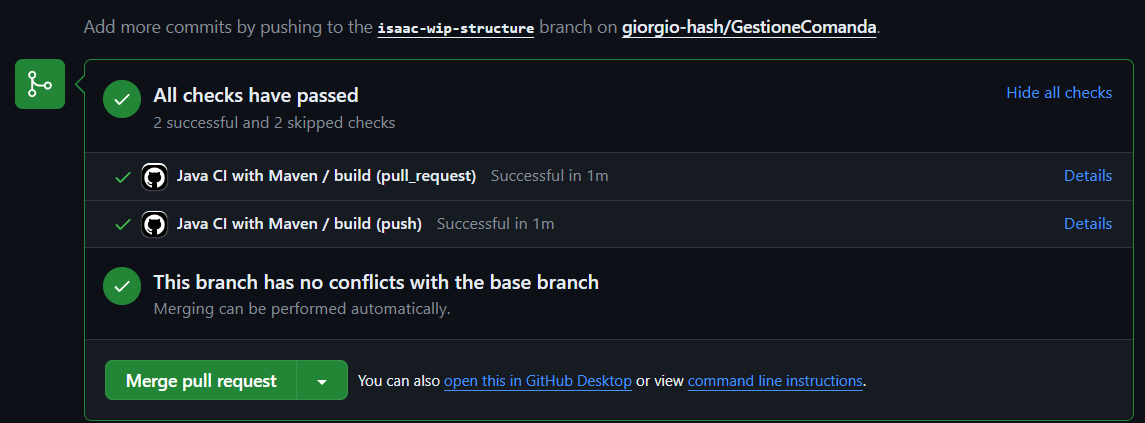
\includegraphics[width=1\linewidth]{iterazione1//images/github_actions_merge.png}
    \caption{CI merge a pull-request}
    \label{fig:cigithubmerge}
\end{figure}
Dalla Figura \vref{fig:cigithubmerge} è possibile notare come all'interno della pull-request sia presente un campo dedicato ai controlli che GitHub Actions ha effettuato e siccome tutti i controlli hanno avuto esito positivo, è possibile procedere al merge della richiesta.
\begin{figure}[H]
    \centering
    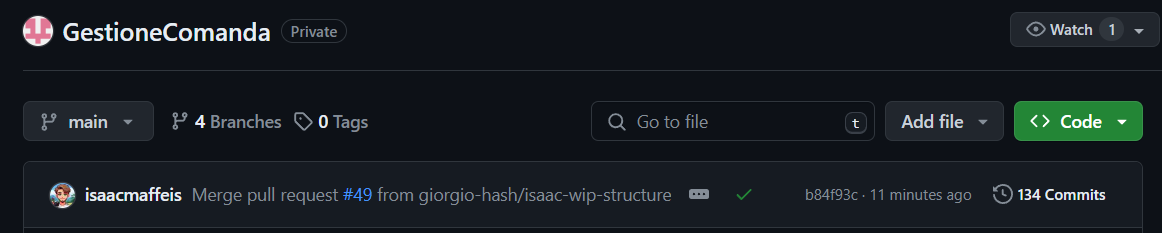
\includegraphics[width=1\linewidth]{iterazione1//images/github_actions_main}
    \caption{CI main check}
    \label{fig:cigithubmain}
\end{figure}
Una volta completato il merge con successo è possibile notare una spunta verde nella repository principale del progetto (Figura \vref{fig:cigithubmain}) che ci informa che allo stato corrente il codice sul main ha passato tutti i test proposti.

\subsection{DTO}
Gli oggetti di trasferimento dati (Data Transfer Object) sono un design pattern utilizzato per trasferire dati tra sottosistemi di un’applicazione software, servono a semplificare e a rendere più efficiente la comunicazione tra i vari livelli di un'applicazione, nel nostro caso tra Interface, Domain e Infrastructure.
\paragraph{Step 1 - Overview:}
Come primo passo ci si è fatti una panoramica leggendo la documentazione ufficiale di Model Mapper \cite{ModelMapperGettingStarted}, ossia la libreria di mapping che useremo per convertire le entità in DTO e viceversa.
\paragraph{Step 2 - Setup:}
Al passo numero due ci si è focalizzati sul setup dell’ambiente di lavoro, andando ad aggiornare inizialmente il file "pom.xml" (Codice \vref{lst:pom-xml5}) con la seguente dipendenza per Model Mapper:
\begin{lstlisting}[language=XML, caption={Aggiornamento dipendenze nel pom.xml per includere model-mapper}, label=lst:pom-xml5]
<dependency>
    <groupId>org.modelmapper</groupId>
    <artifactId>modelmapper</artifactId>
    <version>3.0.0</version>
</dependency>
\end{lstlisting}
E successivamente è stato creato il bean di configurazione nella classe "MapperConfig.java" (Codice \vref{lst:MapperConfig}):
\begin{lstlisting}[style=myJava, 
    caption={Classe di configurazione MapperConfig.java}, label=lst:MapperConfig, 
    emph={[2] LOOSE},
    emphstyle={[2]\color{codeDarkMagenta}},]
@Configuration
public class MapperConfig {

    @Bean
    ModelMapper modelMapper(){
        ModelMapper modelMapper = new ModelMapper();
        modelMapper.getConfiguration().setMatchingStrategy(MatchingStrategies.LOOSE);
        return modelMapper;
    }
}
\end{lstlisting}
La strategia di corrispondenza LOOSE in ModelMapper ignora le differenze di maiuscole/minuscole e gli underscore nei nomi dei campi, considera i campi come corrispondenti anche se i nomi dei campi nell’oggetto sorgente e nell’oggetto destinazione non sono esattamente gli stessi, ma contengono le stesse parole.
\paragraph{Step 3 - DTO:}
Al terzo passo è stata creata la classe DTO per l'entità Ordine che abbiamo definito in precedenza (Codice \vref{lst:OrdineEntity}), semplicemente creando una nuova classe Java (Codice \vref{lst:orderdto}) con gli stessi campi della classe entità, ma senza la logica di business o le annotazioni specifiche dell'entità:
\begin{lstlisting}[style=myJava, 
    caption={Classe DTO per l'entità ordine OrderDTO.java}, label=lst:orderdto, 
    emph={[2] urgenzaCliente, id, idComanda, idPiatto, stato, tOrdinazione },
    emphstyle={[2]\color{codeDarkMagenta}},]
@Data
@AllArgsConstructor
@NoArgsConstructor
@Builder
public class OrdineDTO {

    /**
     * Identificatore dell'ordine
     */
    private int id;

    /**
     * Identificatore della comanda di cui l'ordine fa parte
     */
    private int idComanda;

    /**
     * Identificatore del piatto ordinato dal cliente
     */
    private String idPiatto;

    /**
     * Stato dell'ordine
     * 0: Ordine preso in carico
     * 1: Ordine in coda di preparazione
     * 2: Ordine in preparazione
     * 3: Ordine preparato
     */
    private Integer stato;

    /**
     * Istante temporale in cui viene effettuata l'ordinazione
     * pattern : "yyyy-MM-dd HH:mm:ss.SSS"
     */
    private Timestamp tOrdinazione;

    /**
     * Attributo urgenza del cliente
     * 0 : espresso non urgenza
     * 1 : espresso urgenza
     * 2 : default
     */
    private Integer urgenzaCliente;

}
\end{lstlisting}
\paragraph{Step 4 - Mapper:}
Le classi mapper sono utilizzate per convertire oggetti tra classi entità e DTO (e viceversa), viene inizialmente creata la seguente interfaccia (Codice \vref{lst:mapper}):
\begin{lstlisting}[style=myJava, 
    caption={Interfaccia Mapper.java}, label=lst:mapper, 
    emph={[3] A, B },
    emphstyle={[3]\color{codeCyan}},]
public interface Mapper<A,B> {

    /**
     * Mappa l'oggetto A (Entita') nell'oggetto B (DTO)
     *
     * @param a A Entita'
     * @return B DTO
     */
    B mapTo(A a);

    /**
     * Mappa l'oggetto B (DTO) nell'oggetto A (Entita')
     *
     * @param b B DTO
     * @return A Entita'
     */
    A mapFrom(B b);
\end{lstlisting}
Nella quale con \textit{mapTo} possiamo passare da un'entità ad un DTO, mentre con \textit{mapFrom} possiamo convertire un DTO in un'entità. Viene di conseguenza creata la classe implementazione di questa interfaccia (Codice \vref{lst:OrdineMapper}): 
\begin{lstlisting}[style=myJava, 
    caption={Classe OrdineMapper.java implementazione di ModelMapper.java}, label=lst:OrdineMapper, 
    emph={[2] modelMapper},
    emphstyle={[2]\color{codeDarkMagenta}},
    emph={[3] mapTo, mapFrom },
    emphstyle={[3]\color{codeCyan}},]
@Component
public class OrdineMapper implements Mapper<OrdineEntity, OrdineDTO> {

    private ModelMapper modelMapper;

    public OrdineMapper(ModelMapper modelMapper) {
        this.modelMapper = modelMapper;
    }

    @Override
    public OrdineDTO mapTo(OrdineEntity ordineEntity) {
        return modelMapper.map(ordineEntity,OrdineDTO.class);
    }

    @Override
    public OrdineEntity mapFrom(OrdineDTO ordineDTO) {
        return modelMapper.map(ordineDTO, OrdineEntity.class);
    }
}
\end{lstlisting}
Si può facilmente notare come l'utilizzo di ModelMapper abbia semplificato notevolmente il processo di mapping, infatti ci basta richiamare il metodo \textit{map} offerto dall'istanza modelMapper per svolgere la conversione tra due oggetti.
\paragraph{Step 5 - Testing:}
In questo passo sono stati svolti i test di integrazione (Codice \vref{lst:OrdineMapperTests}) per verificare che la conversione tra entità e DTO sia stata implementata in modo corretto.
\begin{lstlisting}[style=myJava, 
    caption={Test di integrazione OrdineMapperTests.java}, label=lst:OrdineMapperTests, 
    emph={[2] ordineMapper},
    emphstyle={[2]\color{codeDarkMagenta}},
    emph={[3] testMapTo, testMapFrom },
    emphstyle={[3]\color{codeCyan}},]
@SpringBootTest
public class OrdineMapperTests {

    @Autowired
    private OrdineMapper ordineMapper;

    @Test
    public void testMapTo(){
        OrdineEntity ordineEntity = TestDataUtil.createOrdineEntityA();
        OrdineDTO ordineDTO = ordineMapper.mapTo(ordineEntity);
        assertThat(ordineDTO.getId()).isEqualTo(ordineEntity.getId());
        assertThat(ordineDTO.getIdComanda()).isEqualTo(ordineEntity.getIdComanda());
        assertThat(ordineDTO.getStato()).isEqualTo(ordineEntity.getStato());
        assertThat(ordineDTO.getIdPiatto()).isEqualTo(ordineEntity.getIdPiatto());
        assertThat(ordineDTO.getUrgenzaCliente()).isEqualTo(ordineEntity.getUrgenzaCliente());
        assertThat(ordineDTO.getTOrdinazione()).isEqualTo(ordineEntity.getTOrdinazione());
    }

    @Test
    public void testMapFrom(){
        OrdineDTO ordineDTO = TestDataUtil.createOrdineDtoB();
        OrdineEntity ordineEntity = ordineMapper.mapFrom(ordineDTO);
        assertThat(ordineEntity.getId()).isEqualTo(ordineDTO.getId());
        assertThat(ordineEntity.getIdComanda()).isEqualTo(ordineDTO.getIdComanda());
        assertThat(ordineEntity.getStato()).isEqualTo(ordineDTO.getStato());
        assertThat(ordineEntity.getIdPiatto()).isEqualTo(ordineDTO.getIdPiatto());
        assertThat(ordineEntity.getUrgenzaCliente()).isEqualTo(ordineDTO.getUrgenzaCliente());
        assertThat(ordineEntity.getTOrdinazione()).isEqualTo(ordineDTO.getTOrdinazione());
    }
}
\end{lstlisting}
Il metodo \textit{testMapTo()} verifica che l'operazione di mappatura da OrdineEntity a OrdineDTO produca risultati attesi, mentre il metodo \textit{testMapFrom()} verifica che l'operazione inversa di mappatura da OrdineDTO a OrdineEntity produca risultati attesi, in entrambi i casi si considerano dei test di equivalenza su tutti i campi degli oggetti.
\subsection{Interfaccia di Test}
\label{subsec:interfaccia-test}
\paragraph{Step 1 - Overview:}
Come primo passo ci si è fatti una panoramica leggendo la documentazione ufficiale di Spring per costruire un controller REST \cite{spring-rest}.
\paragraph{Step 2 - Setup:}
Al passo numero due ci si è focalizzati sul setup dell’ambiente di lavoro, siccome il microservizio GestioneComanda è sprovvisto di un componente HTTP Controller nella sua Interfaccia (che contiene solo EventController), viene creato un controller di TEST per interagire direttamente con i componenti del servizio per i soli fini di test, per questo motivo viene aggiornato il diagramma UML di Interface di GestioneComanda come segue (Figura \vref{fig:component_comanda_w_test-GestioneComanda__Interface}):
\subsubsection*{zoom-in interface di gestione comanda}
\begin{figure}[H]
	\centering
	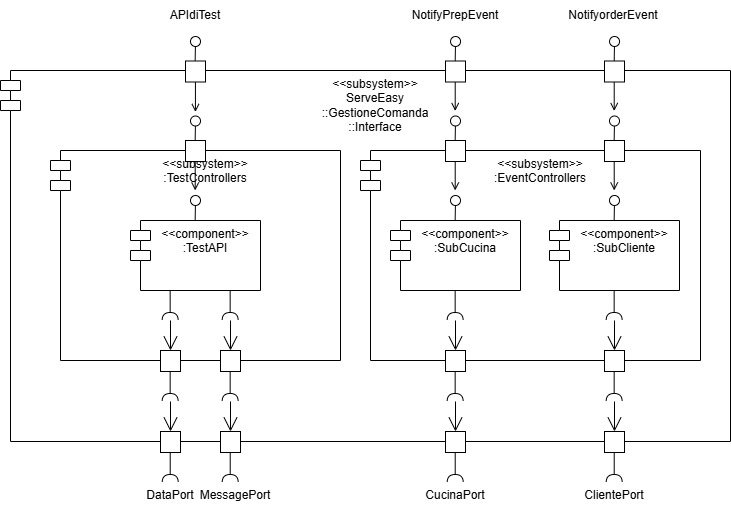
\includegraphics[scale=0.5]{iterazione1/images/component_comanda_w_test-GestioneComanda__Interface.jpg}
	\caption{Component diagram - Gestione Comanda - Interface con Test
    \label{fig:component_comanda_w_test-GestioneComanda__Interface}}
\end{figure}
\begin{itemize}
    \item EventControllers: SubCucina e SubCliente, permettono la ricezione di messaggi tramite message broker dagli altri microservizi.
    \item TestControllers: TestAPI per poter testare le API di Test utilizzando direttamente la DataPort e la MessagePort
\end{itemize}
Risulta importante specificare come il componente \textit{TestAPI} utilizzi direttamente la \textit{DataPort} e la \textit{MessagePort} invece che passare per le interfacce \textit{CucinaPort} e \textit{ClientePort} ovverte dal \textit{Domain}, questo viene fatto per non sconvolgere l'intera struttura dell'applicazione per i soli fini di test, infatti questo componente non verrà utilizzato in produzione.

Successivamente viene aggiornato il file "pom.xml"(Codice \vref{lst:pom-xml6}) con le seguenti dipendenze:
\begin{lstlisting}[language=XML, caption={Aggiornamento dipendenze nel pom.xml per includere spring-web}, label=lst:pom-xml6]
<!-- Spring web -->
<dependency>
    <groupId>org.springframework.boot</groupId>
    <artifactId>spring-boot-starter-web</artifactId>
</dependency>

<!-- Jackson -->
<dependency>
    <groupId>com.fasterxml.jackson.core</groupId>
    <artifactId>jackson-databind</artifactId>
</dependency>

<dependency>
    <groupId>com.fasterxml.jackson.datatype</groupId>
    <artifactId>jackson-datatype-jsr310</artifactId>
</dependency>
\end{lstlisting}
La prima (Spring web) è utilizzata per configurare un'applicazione Spring Boot che presenta un controller REST, include infatti tutte le dipendenze necessarie per avviare un'applicazione web, inclusi Tomcat, Spring MVC e altre dipendenze di supporto.
Mentre le seconde (Jackson) sono dipendenze Jackson utilizzate per la serializzazione e deserializzazione degli oggetti Java in formato JSON e viceversa fondamentali quando si sviluppano servizi RESTful con Spring Boot.
\paragraph{Step 3 - API:}
In questo passo vengono definite le API di Test che dovrà esporre il TestController, viene quindi creata l'interfaccia (Codice \vref{lst:testapiIF}) annotandola con \textit{@RequestMapping("/test")}, il che significa che tutti gli endpoint definiti all'interno di questa interfaccia sono raggiungibili tramite l'URI base "/test":
\begin{lstlisting}[style=myJava, 
    caption={Interfaccia TestAPI.java}, label=lst:testapiIF, 
    emph={[2] },
    emphstyle={[2]\color{codeDarkMagenta}},
    emph={[3] addOrdine, getOrdine, getAllOrdersByIdComanda, partialUpdateOrdine, deleteOrder, sendOrderEvent, getMessageFromTopicSendOrderEvent, sendNotifyOrderEvent, getMessageFromTopicNotifyOrderEvent, sendNotifyPrepEvent, getMessageFromTopicNotifyPrepEvent },
    emphstyle={[3]\color{codeCyan}},]
@RequestMapping("/test")
public interface TestAPI {

    /**
     * Salva nel database l'oggetto ordine dato un ordineDTO
     *
     * @param ordineDTO DTO dell'entita' ordine da salvare
     * @return entita' risposta che contiene l'oggetto creato e una risposta HTTP associata
     */
    @PostMapping(path="/order")
    ResponseEntity<OrdineDTO> addOrdine(@RequestBody OrdineDTO ordineDTO);

    /**
     * Restituisci l'ordine corrispondente all'id dato in input
     *
     * @param id id dell'ordine riqchiesto
     * @return entita' risposta che contiene l'oggetto richiesto e una risposta HTTP associata
     */
    @GetMapping(path="order/{id}")
    ResponseEntity<OrdineDTO> getOrdine(@PathVariable int id);

    /**
     * Restituisce una lista con tutti gli ordini relativi a una data comanda
     *
     * @param idComanda id della comanda di riferimento
     * @return entita' risposta che contiene la lista richiesta e una risposta HTTP associata
     */
    @GetMapping(path = "orders/{idComanda}")
    ResponseEntity<List<OrdineDTO>> getAllOrdersByIdComanda(@PathVariable int idComanda);

    /**
     * Aggiornamento parziale dell'entita' ordine, e' possibile fornire solamente gli oggetti da aggiornare
     *
     * @param id id dell'ordine da aggiornare
     * @param ordineDTO oggetto DTO con le modifiche da effettuare
     * @return entita' risposta che contiene l'oggetto aggiornato e una risposta HTTP associata
     */
    @PatchMapping(path="order/{id}")
    ResponseEntity<OrdineDTO> partialUpdateOrdine(@PathVariable int id, @RequestBody OrdineDTO ordineDTO);

    /**
     * Cancella l'ordine con il dato ID dal databse
     *
     * @param id id dell'ordine da eliminare
     * @return entita' risposta che contiene la risposta HTTP associata
     */
    @DeleteMapping(path = "/order/{id}")
    ResponseEntity deleteOrder(@PathVariable("id") int id);

    /**
     * Espone una API di POST con la quale e' possibile iniettare all'interno del broker oggetti al fine di test
     * Si testa il topic sendOrderEvent da gestione comanda verso gestione cucina
     *
     * @param ordineDTO contenuto dell'oggetto da iniettare
     * @return entita' risposta che contiene l'oggetto creato e una risposta HTTP associata
     * @throws JsonProcessingException eccezione sollevata dalla serializzazione
     */
    @PostMapping(path = "/sendorderevent")
    ResponseEntity<OrdineDTO> sendOrderEvent(@RequestBody OrdineDTO ordineDTO) throws JsonProcessingException;

    /**
     * Espone una API di GET con la quale e' possibile ottenere l'ultimo messaggio letto sul topic SendOrderEvent
     * Si testa il topic notifyPrepEvent da gestione cucina verso gestione comanda
     * @return entita' risposta che contiene l'oggetto richiesto e una risposta HTTP associata
     */
    @GetMapping(path = "/sendorderevent")
    ResponseEntity<String> getMessageFromTopicSendOrderEvent();

    /**
     * Espone una API di POST con la quale e' possibile iniettare all'interno del broker oggetti al fine di test
     * Si testa il topic notifyOrderEvent da gestione cliente verso gestione comanda
     * @param notificaOrdineDTO contenuto dell'oggetto da iniettare
     * @return entita' risposta che contiene l'oggetto creato e una risposta HTTP associata
     * @throws JsonProcessingException eccezione sollevata dalla serializzazione
     */
    @PostMapping(path = "/notifyorderevent")
    ResponseEntity<NotificaOrdineDTO> sendNotifyOrderEvent(@RequestBody NotificaOrdineDTO notificaOrdineDTO) throws JsonProcessingException;

    /**
     * Espone una API di GET con la quale e' possibile ottenere l'ultimo messaggio letto sul topic NotifyOrderEvent
     * Si testa il topic notifyPrepEvent da gestione cucina verso gestione comanda
     * @return entita' risposta che contiene l'oggetto richiesto e una risposta HTTP associata
     */
    @GetMapping(path = "/notifyorderevent")
    ResponseEntity<NotificaOrdineDTO> getMessageFromTopicNotifyOrderEvent();

    /**
     * Espone una API di POST con la quale e' possibile iniettare all'interno del broker oggetti al fine di test
     * Si testa il topic notifyPrepEvent da gestione cucina verso gestione comanda
     * @param notificaPrepOrdineDTO contenuto dell'oggetto da iniettare
     * @return entita' risposta che contiene l'oggetto creato e una risposta HTTP associata
     * @throws JsonProcessingException eccezione sollevata dalla serializzazione
     */
    @PostMapping(path = "/notifyprepevent")
    ResponseEntity<NotificaPrepOrdineDTO> sendNotifyPrepEvent(@RequestBody NotificaPrepOrdineDTO notificaPrepOrdineDTO) throws JsonProcessingException;

    /**
     * Espone una API di GET con la quale e' possibile ottenere l'ultimo messaggio letto sul topic NotifyPrepEvent
     * Si testa il topic notifyPrepEvent da gestione cucina verso gestione comanda
     * @return entita' risposta che contiene l'oggetto richiesto e una risposta HTTP associata
     */
    @GetMapping(path = "/notifyprepevent")
    ResponseEntity<NotificaPrepOrdineDTO> getMessageFromTopicNotifyPrepEvent();
}
\end{lstlisting}
In questo modo definiamo una serie di endpoint per API REST. Ogni metodo dell'interfaccia rappresenta un endpoint dell'API e specifica il tipo di richiesta HTTP supportata, il percorso dell'endpoint e gli eventuali parametri richiesti.
\paragraph{Step 4 - RestController:}
A questo punto possiamo costruire l'implementazione dell'interfaccia TestAPI appena definita (Codice \vref{lst:testapiIF}) andando a creare un controller REST di test (Codice \vref{lst:restcontrollertest}):
\begin{lstlisting}[style=myJava, 
    caption={Classe REST Controller di test TestController.java}, label=lst:restcontrollertest, 
    emph={[2] ordineMapper, testService, dataPort, topic_notifyOrderEvent, topic_notifyPrepEvent},
    emphstyle={[2]\color{codeDarkMagenta}},
    emph={[3] addOrdine, getOrdine, getAllOrdersByIdComanda, partialUpdateOrdine, deleteOrder, sendOrderEvent, getMessageFromTopicSendOrderEvent, sendNotifyOrderEvent, getMessageFromTopicNotifyOrderEvent, sendNotifyPrepEvent, getMessageFromTopicNotifyPrepEvent },
    emphstyle={[3]\color{codeCyan}},]
@RestController
public class TestController implements TestAPI {
    private TestService testService;
    private Mapper<OrdineEntity, OrdineDTO> ordineMapper;
    private DataPort dataPort;
    @Value("${spring.kafka.consumer.gestioneCliente.topic}")
    private String topic_notifyOrderEvent;
    @Value("${spring.kafka.consumer.gestioneCucina.topic}")
    private String topic_notifyPrepEvent;
    
    @Autowired
    public TestController(TestService testService, Mapper<OrdineEntity, OrdineDTO> ordineMapper, DataPort dataPort) {
        this.testService = testService;
        this.ordineMapper = ordineMapper;
        this.dataPort = dataPort;
    }

    @Override
    public ResponseEntity<OrdineDTO> addOrdine(OrdineDTO ordineDTO) {
        OrdineEntity ordineEntity = ordineMapper.mapFrom(ordineDTO);
        OrdineEntity savedOrdineEntity = dataPort.saveOrder(ordineEntity);
        OrdineDTO savedOrdineDTO = ordineMapper.mapTo(savedOrdineEntity);
        return new ResponseEntity<>(savedOrdineDTO, HttpStatus.CREATED);
    }

    @Override
    public ResponseEntity<OrdineDTO> getOrdine(int id) {
        Optional<OrdineEntity> ordineEntity = dataPort.getOrderById(id);
        if(ordineEntity.isPresent()){
            OrdineDTO ordineDTO = ordineMapper.mapTo(ordineEntity.get());
            return new ResponseEntity<>(ordineDTO, HttpStatus.OK);
        }
        return new ResponseEntity<>(HttpStatus.NOT_FOUND);
    }

    @Override
    public ResponseEntity<OrdineDTO> partialUpdateOrdine(@PathVariable int id, @RequestBody OrdineDTO ordineDTO) {
        if(!dataPort.isOrderExist(id))
            return new ResponseEntity<>(HttpStatus.NOT_FOUND);

        OrdineEntity ordineEntity = ordineMapper.mapFrom(ordineDTO);
        OrdineEntity updatedEntity = dataPort.updateOrder(id, ordineEntity);

        return new ResponseEntity<>(ordineMapper.mapTo(updatedEntity),HttpStatus.OK);
    }

    @Override
    public ResponseEntity<List<OrdineDTO>> getAllOrdersByIdComanda(int idComanda) {
        List<OrdineEntity> ordini = dataPort.findAllOrdersByIdComanda(idComanda);
        if(!ordini.isEmpty())
            return new ResponseEntity<>(ordini.stream()
                    .map(ordineMapper::mapTo)
                    .collect(Collectors.toList()),HttpStatus.OK);
        else
            return new ResponseEntity<>(HttpStatus.NOT_FOUND);
    }

    @Override
    public ResponseEntity deleteOrder(@PathVariable("id") int id) {
        dataPort.deleteOrder(id);
        return new ResponseEntity(HttpStatus.NO_CONTENT);
    }

    @Override
    public ResponseEntity<OrdineDTO> sendOrderEvent(@RequestBody OrdineDTO ordineDTO) throws JsonProcessingException {
        OrdineEntity ordineEntity = ordineMapper.mapFrom(ordineDTO);
        OrdineEntity savedOrdineEntity = dataPort.saveOrder(ordineEntity);
        OrdineDTO savedOrdineDTO = ordineMapper.mapTo(savedOrdineEntity);
        testService.sendMessageToTopicSendOrderEvent(savedOrdineDTO);
        return new ResponseEntity<>(savedOrdineDTO, HttpStatus.CREATED);
    }

    @Override
    public ResponseEntity<String> getMessageFromTopicSendOrderEvent() {
        Optional<String> message = testService.peekFromSendOrderEvent();
        if(message.isPresent())
            return new ResponseEntity<>(message.get(), HttpStatus.OK);
        else
            return new ResponseEntity<>(HttpStatus.NOT_FOUND);
    }

    @Override
    public ResponseEntity<NotificaOrdineDTO> sendNotifyOrderEvent(@RequestBody NotificaOrdineDTO notificaOrdineDTO) throws JsonProcessingException {
        String message = testService.serializeObject(notificaOrdineDTO);
        testService.sendMessageToTopic(message, topic_notifyOrderEvent);
        return new ResponseEntity<>(notificaOrdineDTO, HttpStatus.CREATED);
    }

    @Override
    public ResponseEntity<NotificaOrdineDTO> getMessageFromTopicNotifyOrderEvent() {
        Optional<NotificaOrdineDTO> message = testService.peekFromNotifyOrderEvent();
        if(message.isPresent())
            return new ResponseEntity<>(message.get(), HttpStatus.OK);
        else
            return new ResponseEntity<>(HttpStatus.NOT_FOUND);
    }

    @Override
    public ResponseEntity<NotificaPrepOrdineDTO> sendNotifyPrepEvent(@RequestBody NotificaPrepOrdineDTO notificaPrepOrdineDTO) throws JsonProcessingException {
        String message = testService.serializeObject(notificaPrepOrdineDTO);
        testService.sendMessageToTopic(message, topic_notifyPrepEvent);
        return new ResponseEntity<>(notificaPrepOrdineDTO, HttpStatus.CREATED);
    }

    @Override
    public ResponseEntity<NotificaPrepOrdineDTO> getMessageFromTopicNotifyPrepEvent() {
        Optional<NotificaPrepOrdineDTO> message = testService.peekFromNotifyPrepEvent();
        if(message.isPresent())
            return new ResponseEntity<>(message.get(), HttpStatus.OK);
        else
            return new ResponseEntity<>(HttpStatus.NOT_FOUND);
    }
}
\end{lstlisting}
Questa classe è un controller Spring MVC che gestisce le richieste HTTP relative alle operazioni CRUD (Create, Read, Update, Delete) sull'entità ordine del database passando per i corrispettivi DTO e gestisce le richiesti di operazioni sui topic del message broker, utilizzando il pattern architetturale API RESTful.
Per una documentazione più dettagliata su ogni singola API si rimanda al capitolo \vref{sec:docapi}.
\paragraph{Step 5 - Testing:}
In questo passo ci siamo occupati di testare il REST Controller appena creato, lo abbiamo fatto utilizzando MockMVC \cite{spring-mvc-test}, ovvero una classe fornita da Spring MVC Test Framework che consente di simulare le richieste HTTP e testare il comportamento dei controller Spring MVC senza dover effettivamente avviare un server HTTP.
\begin{lstlisting}[style=myJava, 
    caption={Classe Test per il REST Controller di test TestControllerTests.java}, label=lst:testrestcontrollertest, 
    emph={[2] objectMapper, mockMvc , dataPort, topic_notifyOrderEvent, topic_notifyPrepEvent, embeddedKafka, AFTER_EACH_TEST_METHOD, APPLICATION_JSON},
    emphstyle={[2]\color{codeDarkMagenta}},
    emph={[3] testThatGetOrderReturnsHttpStatus200WhenOrderExist, testThatGetOrderReturnsHttpStatus404WhenNoOrderExists, testThatGetOrderReturnsOrderWhenOrderExist  },
    emphstyle={[3]\color{codeCyan}},]
@SpringBootTest
@EnableKafka
@DirtiesContext(classMode = DirtiesContext.ClassMode.AFTER_EACH_TEST_METHOD)
@EmbeddedKafka(partitions = 1,
        controlledShutdown = false,
        brokerProperties = { "listeners=PLAINTEXT://localhost:9092", "port=9092" },
        topics = {"${spring.kafka.producer.topic}",
                "${spring.kafka.consumer.gestioneCliente.topic}" ,
                "${spring.kafka.consumer.gestioneCucina.topic}" })
@AutoConfigureMockMvc
public class TestControllerTests {
    @Autowired
    private MockMvc mockMvc;
    @Autowired
    private ObjectMapper objectMapper;
    @Autowired
    private DataPort dataPort;
    @Autowired
    private EmbeddedKafkaBroker embeddedKafka;
    @Value("${spring.kafka.consumer.gestioneCliente.topic}")
    private String topic_notifyOrderEvent;
    @Value("${spring.kafka.consumer.gestioneCucina.topic}")
    private String topic_notifyPrepEvent;
    @Value("${spring.kafka.producer.topic}")
    private String topic_sendOrderEvent;

    @Test
    public void testThatGetOrderReturnsHttpStatus200WhenOrderExist() throws Exception {
        OrdineEntity ordineEntity = TestDataUtil.createOrdineEntityB();
        dataPort.saveOrder(ordineEntity);
        mockMvc.perform(MockMvcRequestBuilders.get("/test/order/1").contentType(MediaType.APPLICATION_JSON)).andExpect(MockMvcResultMatchers.status().isOk());
    }

    @Test
    public void testThatGetOrderReturnsHttpStatus404WhenNoOrderExists() throws Exception {
        mockMvc.perform(MockMvcRequestBuilders.get("/test/order/99").contentType(MediaType.APPLICATION_JSON)).andExpect(MockMvcResultMatchers.status().isNotFound());
    }

    @Test
    public void testThatGetOrderReturnsOrderWhenOrderExist() throws Exception {
        OrdineEntity ordineEntity = TestDataUtil.createOrdineEntityB();
        dataPort.saveOrder(ordineEntity);

        mockMvc.perform(
                MockMvcRequestBuilders.get("/test/order/1")
                        .contentType(MediaType.APPLICATION_JSON)
        ).andExpect(
                MockMvcResultMatchers.jsonPath("$.id").value(1)
        ).andExpect(
                MockMvcResultMatchers.jsonPath("$.idComanda").value(ordineEntity.getIdComanda())
        ).andExpect(
                MockMvcResultMatchers.jsonPath("$.idPiatto").value(ordineEntity.getIdPiatto())
        ).andExpect(
                MockMvcResultMatchers.jsonPath("$.stato").value(ordineEntity.getStato())
        ).andExpect(
                MockMvcResultMatchers.jsonPath("$.urgenzaCliente").value(ordineEntity.getUrgenzaCliente()));
    }
    ...
}
\end{lstlisting}
Vengono mostrati per semplicità solamente i casi di test che riguardano la API di GET (\textit{getOrdine(int id)} che richiede l'ordine dato un id), si testa lo stato della risposta e l'oggetto ricevuto, i restanti casi di test sono analoghi.
Si nota come viene utilizzato mockMVC: si utilizza \textit{perform()} per simulare richieste HTTP, \textit{andExpect()} per verificare lo stato della risposta e \textit{andDO()} per ispezionare la risposta.
\paragraph{Step 6 - Postman:}
A questo punto vengono testate le API tramite Postman, si rimanda nuovamente alla sezione \vref{sec:docapi} per una documentazione dettagliata di ogni API.
È stato creato un workspace condiviso tra i membri del team, nel quale si sono salvate tutte le API da testare, viene mostraro un esempio applicativo (in Figura \vref{fig:postman-screen}):
\begin{figure}[H]
    \centering
    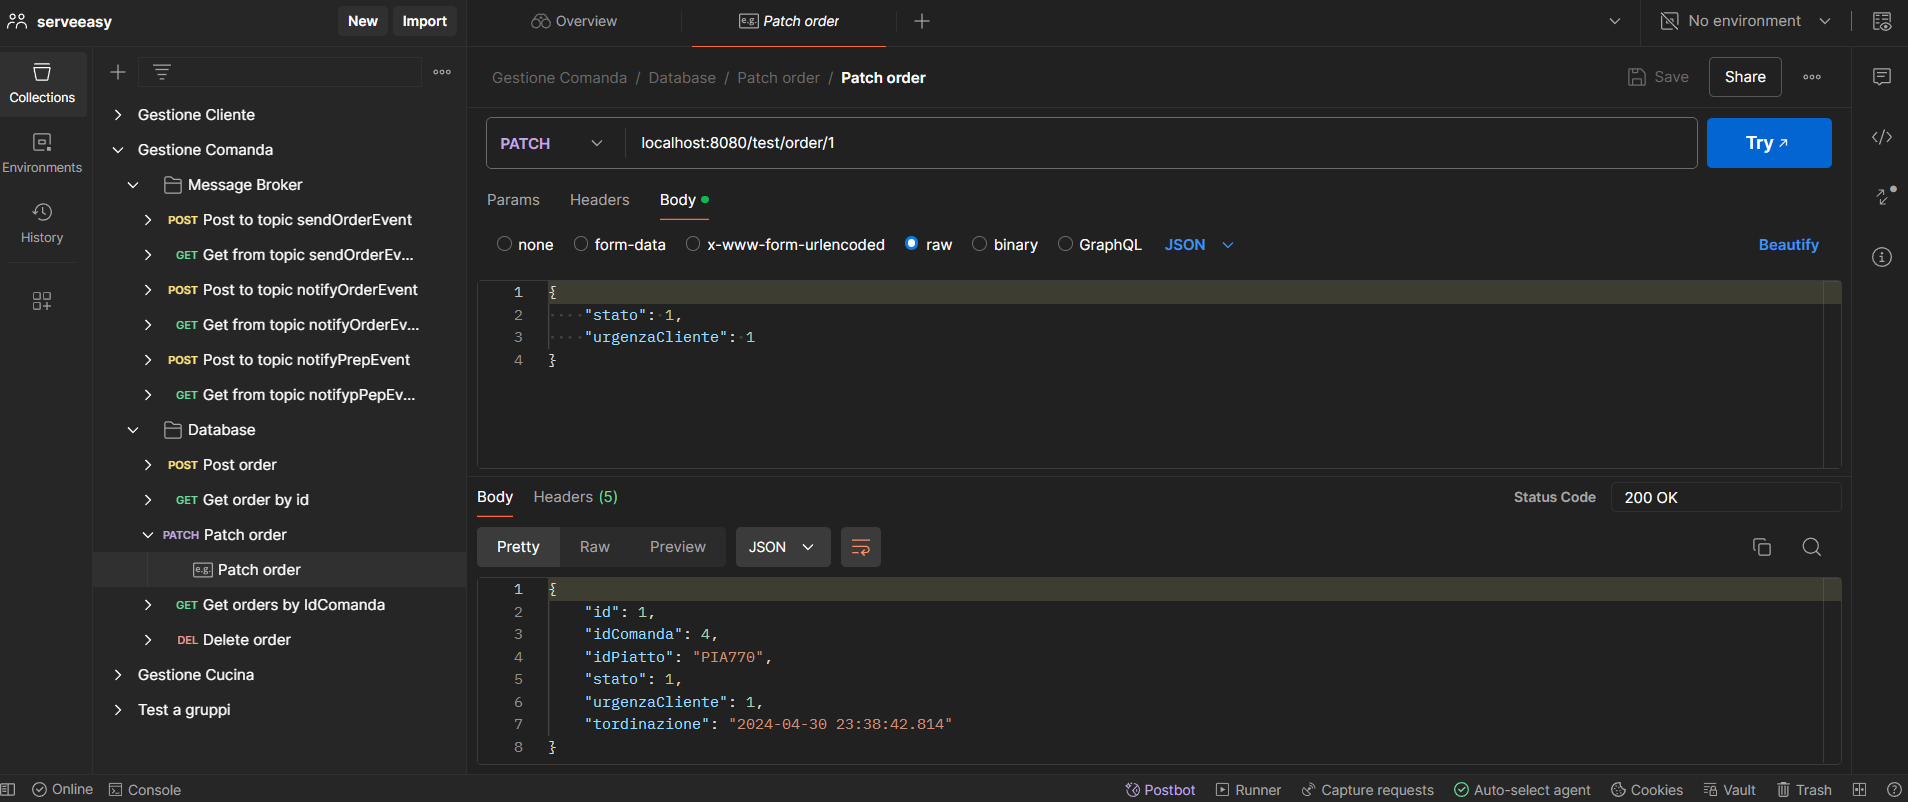
\includegraphics[width=1\linewidth]{iterazione1/images/postman-screen.png}
    \caption{Esempio applicativo Postman}
    \label{fig:postman-screen}
\end{figure}
In questo esempio viene effettuata una richiesta di PATCH di aggiornamento parziale di un ordine, viene specificata la variabile di percorso \textit{id=1} e il corpo della richiesta, ossia il JSON con il quale sono descritti i campi di \textit{stato} e \textit{urgenzaCliente} da aggiornare. Si può notare il codice di risposta 200 OK che viene restituito quando una richiesta HTTP è stata completata con successo e il corpo della risposta, ovvero un JSON contenente l'oggetto OrdineDTO serializzato.
\clearpage
    \section{Deployment dei microservizi con Docker}

\subsection{Healthcheck}
L’healthcheck è una funzionalità di Docker che permette di definire dei controlli di salute sul container: specificando un comando da mandare in azione periodicamente, Docker controlla se il container è "vivo e in salute". Per capire se l'applicazione è sia "viva"(quindi online) che "in salute"(e quindi operativa), risulta cruciale la scelta del comando da mandare periodicamente in azione.

Alcuni applicativi, come il DBMS MariaDB adottato, contengono degli script dediti al controllo della salute del sistema (nel caso di MariaDB, essa contiene nel suo filesystem \textit{healthcheck.sh}, dedita proprio a questa operazione), mentre altri utilizzano delle operazioni note.

I microservizi in Spring Boot, in particolare, hanno la possibilità di installare la dipendenza \textit{Actuator}\cite{halthcheck} che consente l'healthcheck. Tale dipendenza espone una API apposita per restituire lo stato in salute dell'applicativo. E' stato possibile quindi utilizzare l'API \texttt{/actuator/health} del microservizio per effettuare un controllo periodico del suo stato in salute. 

L'healthcheck può inoltre servire per valutare la salute complessiva della rete di microservizi: è possibile introdurre un vincolo di dipendenza tra i componenti di sistema affinchè un certo container vada online solo se i container da cui è dipendente sono "vivi e in salute".

\subsection{Setup della rete di microservizi}
Viene impostato il \textit{docker-compose.yaml} esplicitando i microservizi che compongono l'architettura. Spring Boot dà la possibilità di impostare le variabili ambientali sui container Docker Compose, in modo da sovrascrivere le proprietà definite nel \textit{application.yaml} e \textit{application.properties}. 
In questo modo, è possibile riadattare l'esecuzione dei microservizi per assumere un'impostazione su misura per la runtime in rete.

\begin{lstlisting}[language=docker-compose,caption={GestioneCucina con healthcheck, dipendenze e variabili sovrascritte},label=lst:healthcheck]
|@\color{codeMediumDarkblue}\textbf{GestioneCucina}|@:
    image: gchirico1/gestione_cucina:latest
    container_name: GestioneCucina
    restart: always
    environment:
      |@\color{codeMediumDarkblue}\textbf{SERVER\_PORT}|@: 8080
      |@\color{codeMediumDarkblue}\textbf{SERVER\_ADDRESS}|@: 0.0.0.0
      |@\color{codeMediumDarkblue}\textbf{SPRING\_DATASOURCE\_URL}|@: jdbc:mariadb://db:3306/serveeasy
      |@\color{codeMediumDarkblue}\textbf{SPRING\_KAFKA\_BOOTSTRAP-SERVERS}|@: broker:29092 #plaintext_internal
    depends_on:
      |@\color{codeMediumDarkblue}\textbf{broker}|@:
        |@\color{codeMediumDarkblue}\textbf{condition}|@: service_healthy
      |@\color{codeMediumDarkblue}\textbf{db}|@:
        |@\color{codeMediumDarkblue}\textbf{condition}|@: service_healthy
    |@\color{codeMediumDarkblue}\textbf{healthcheck}|@:
        |@\color{codeMediumDarkblue}\textbf{test}|@: "curl --fail --silent localhost:8080/actuator/health | grep UP || exit 1"
        |@\color{codeMediumDarkblue}\textbf{interval}|@: 20s
        |@\color{codeMediumDarkblue}\textbf{timeout}|@: 5s
        |@\color{codeMediumDarkblue}\textbf{start\_period}|@: 40s
    |@\color{codeMediumDarkblue}\textbf{expose}|@:
      - "8080"
    ports:
      - "8082:8080"
\end{lstlisting}

\subsection{Attivazione della rete di microservizi}
Oltre al comando \texttt{docker compose up}, è possibile attivare e gestire la rete da Intellij IDEA. Quest'ultima modalità è risultata molto più comoda per il controllo della salute e delle attività della rete: il cruscotto offerto dall'IDE consente, infatti, una visuale completa e dettagliata di ogni log in tempo reale. 

Attivato il \textit{docker-compose.yml}, vengono scaricati i microservizi da Dockerhub e attivati i container seguendo la sequenza specificata attraverso le dipendenze.

\begin{figure}[htbp]
	\centering
	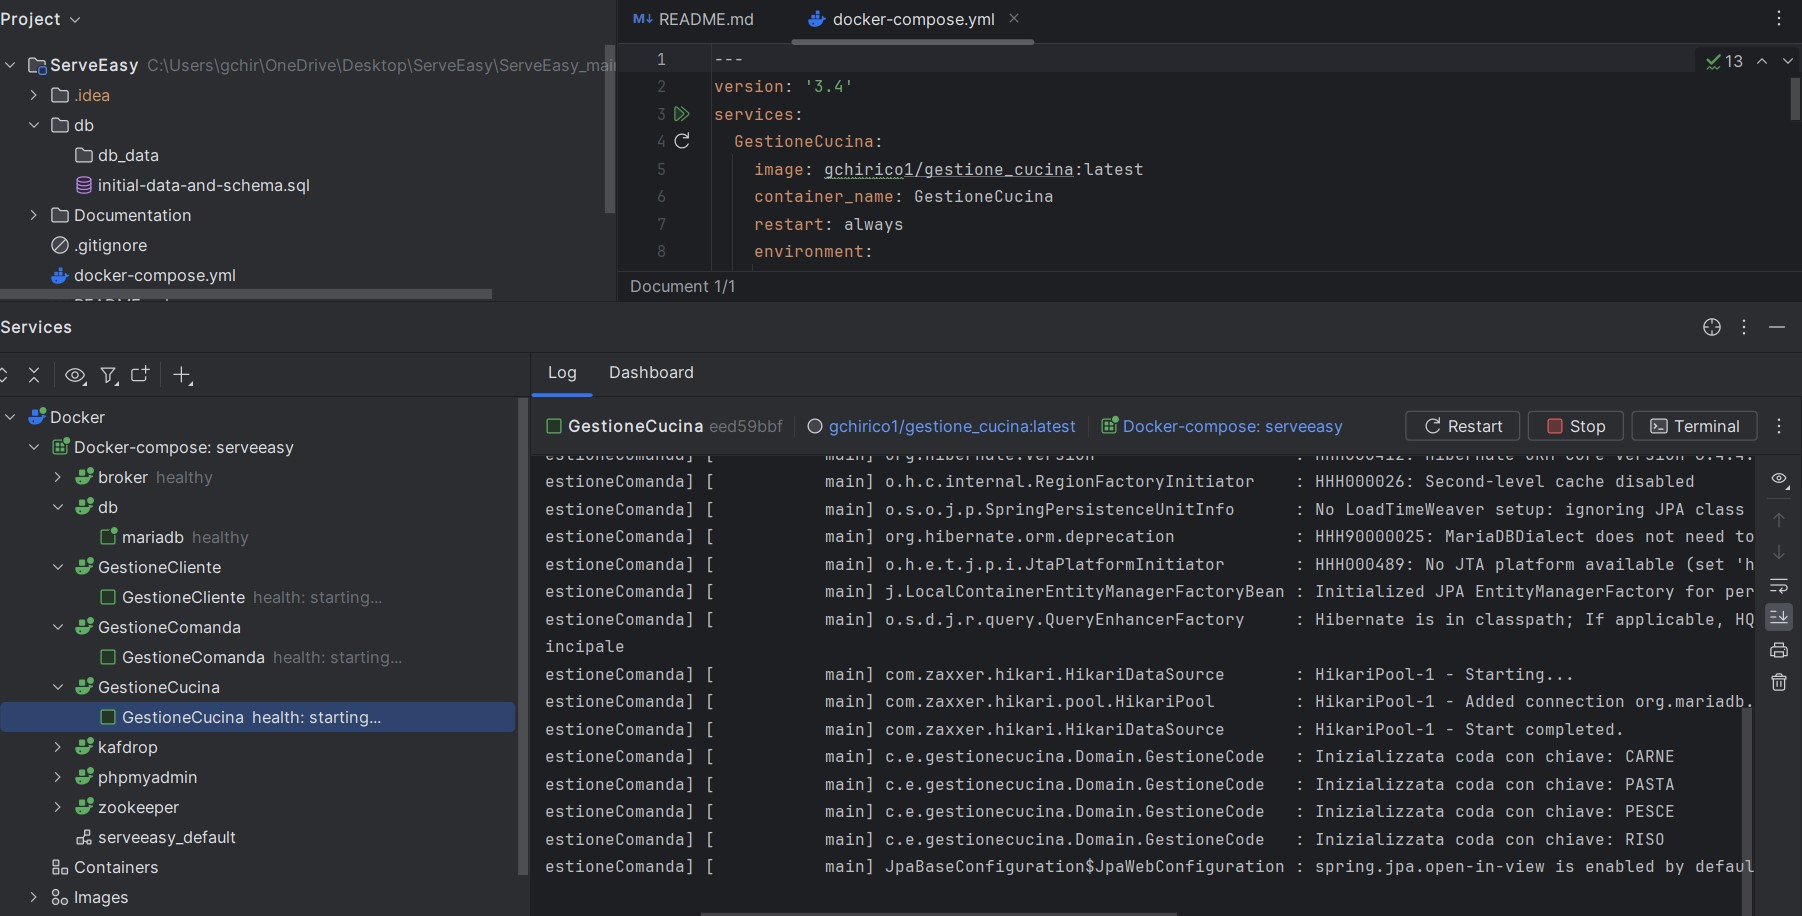
\includegraphics[scale=0.40]{iterazione1/images/startup.jpg}
	\caption{Startup della rete, inizializzazione code in GestioneCucina
 \label{fig:startupcucina}}
\end{figure}
\clearpage
    \section{Documentazione delle API}
\label{sec:docapi}
Le API esposte dai microservizi sono state testate tramite \href{https://www.postman.com/}{postman} utilizzato in locale tramite \href{https://www.postman.com/downloads/postman-agent/}{postman agent} creando un workspace condiviso tra il team.

Come discusso nella sezione \vref{subsec:interfaccia-test}, il microservizio GestioneComanda è sprovvisto di un componente HTTP Controller nella sua Interfaccia (che contiene solo EventController), è quindi stato creato un controller di TEST per interagire direttamente con i componenti del servizio ai soli fini di test.

Viene di seguito allegata la documentazione delle API redatta utilizzando lo strumento \href{https://www.postman.com/api-documentation-tool/}{documenter.getpostman}, link ai documenti ufficiali con anche esempi:
\begin{itemize}
    \item Gestione Comanda: \href{https://documenter.getpostman.com/view/32004409/2sA3JDhkaG}{https://documenter.getpostman.com/view/32004409/2sA3JDhkaG}
    \item Gestione Cliente: \href{https://documenter.getpostman.com/view/32004409/2sA3JFBQDv}{https://documenter.getpostman.com/view/32004409/2sA3JFBQDv}
    \item Gestione Cucina: \href{https://documenter.getpostman.com/view/32004409/2sA3JF9iav}{https://documenter.getpostman.com/view/32004409/2sA3JF9iav}
\end{itemize}

%\subsection{API di Gestione Comanda}
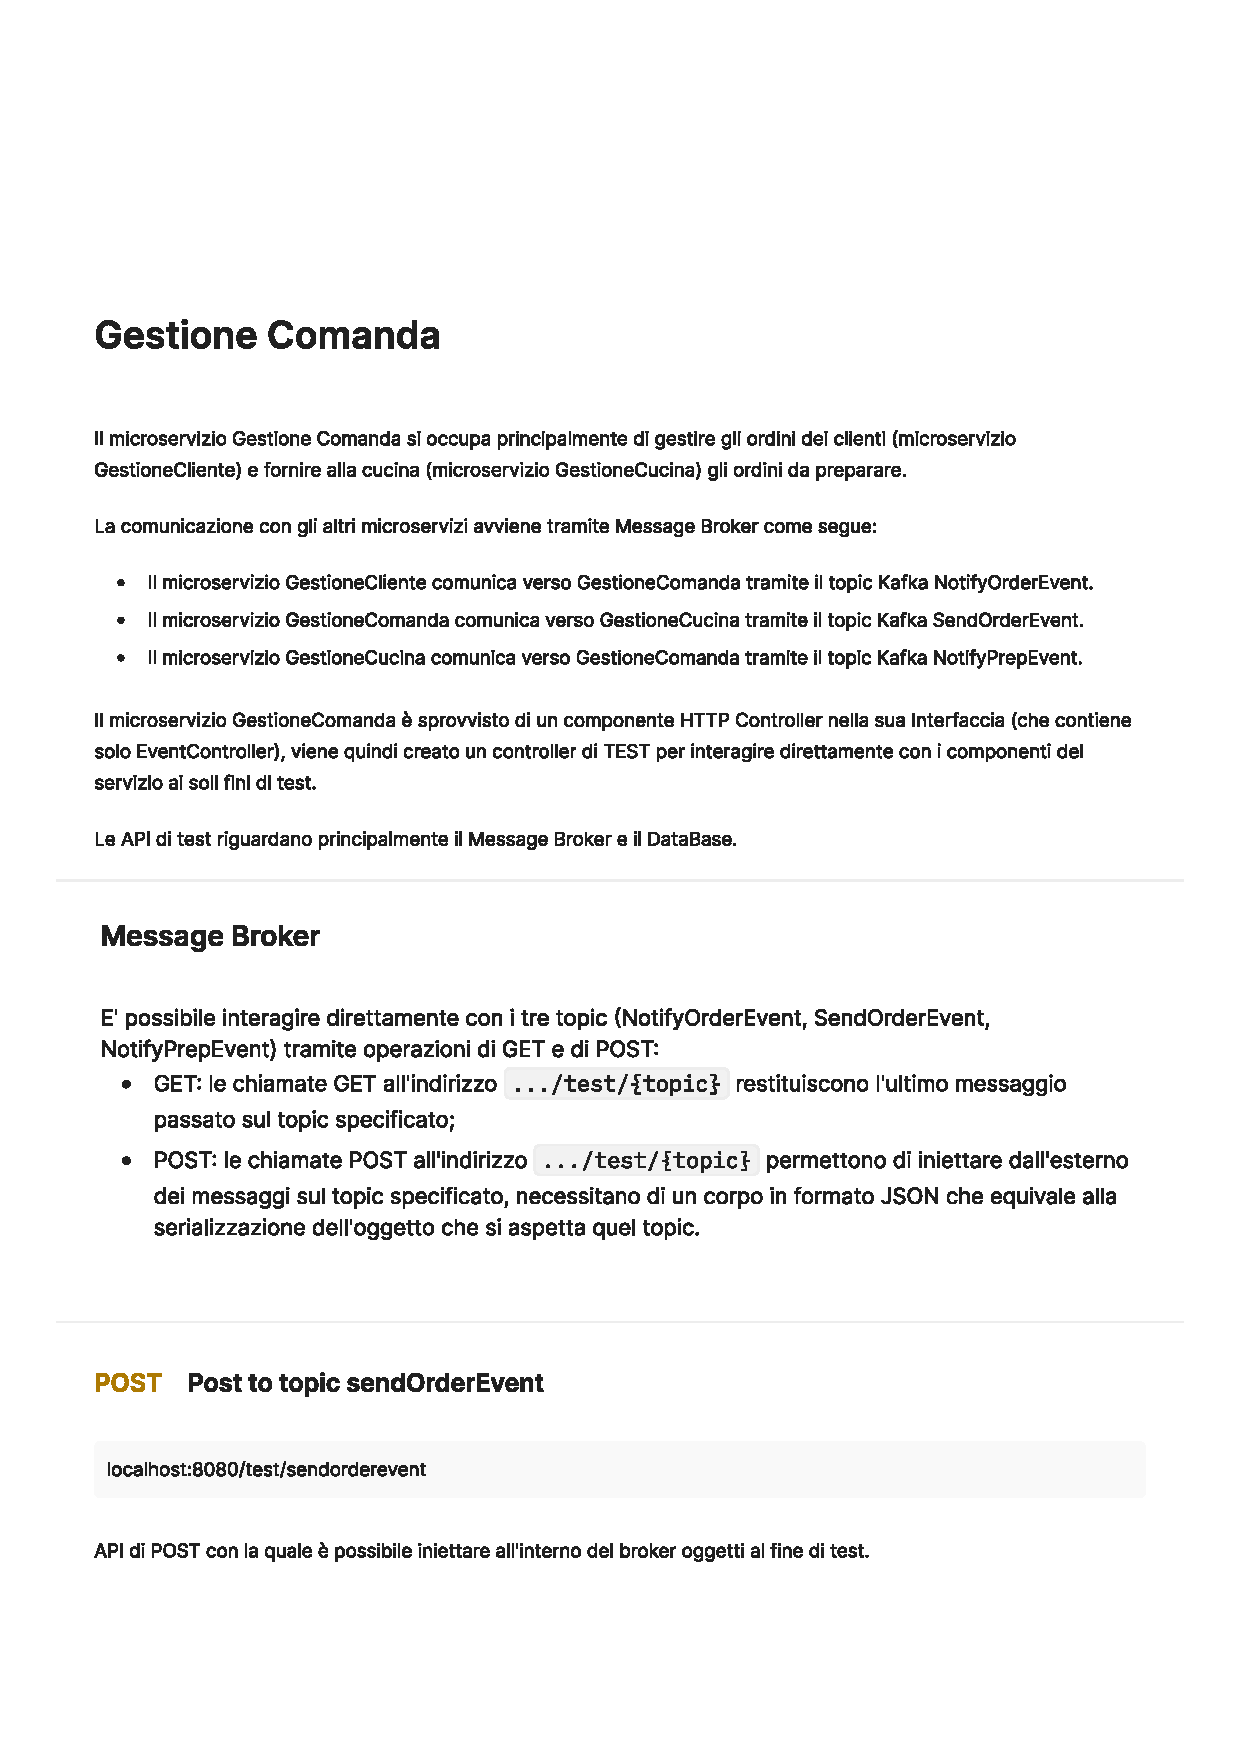
\includepdf[pages=-,pagecommand={\thispagestyle{fancy}},fitpaper=true]{iterazione1/resources/Postman-GestioneComanda.pdf}

%\subsection{API di Gestione Cliente}
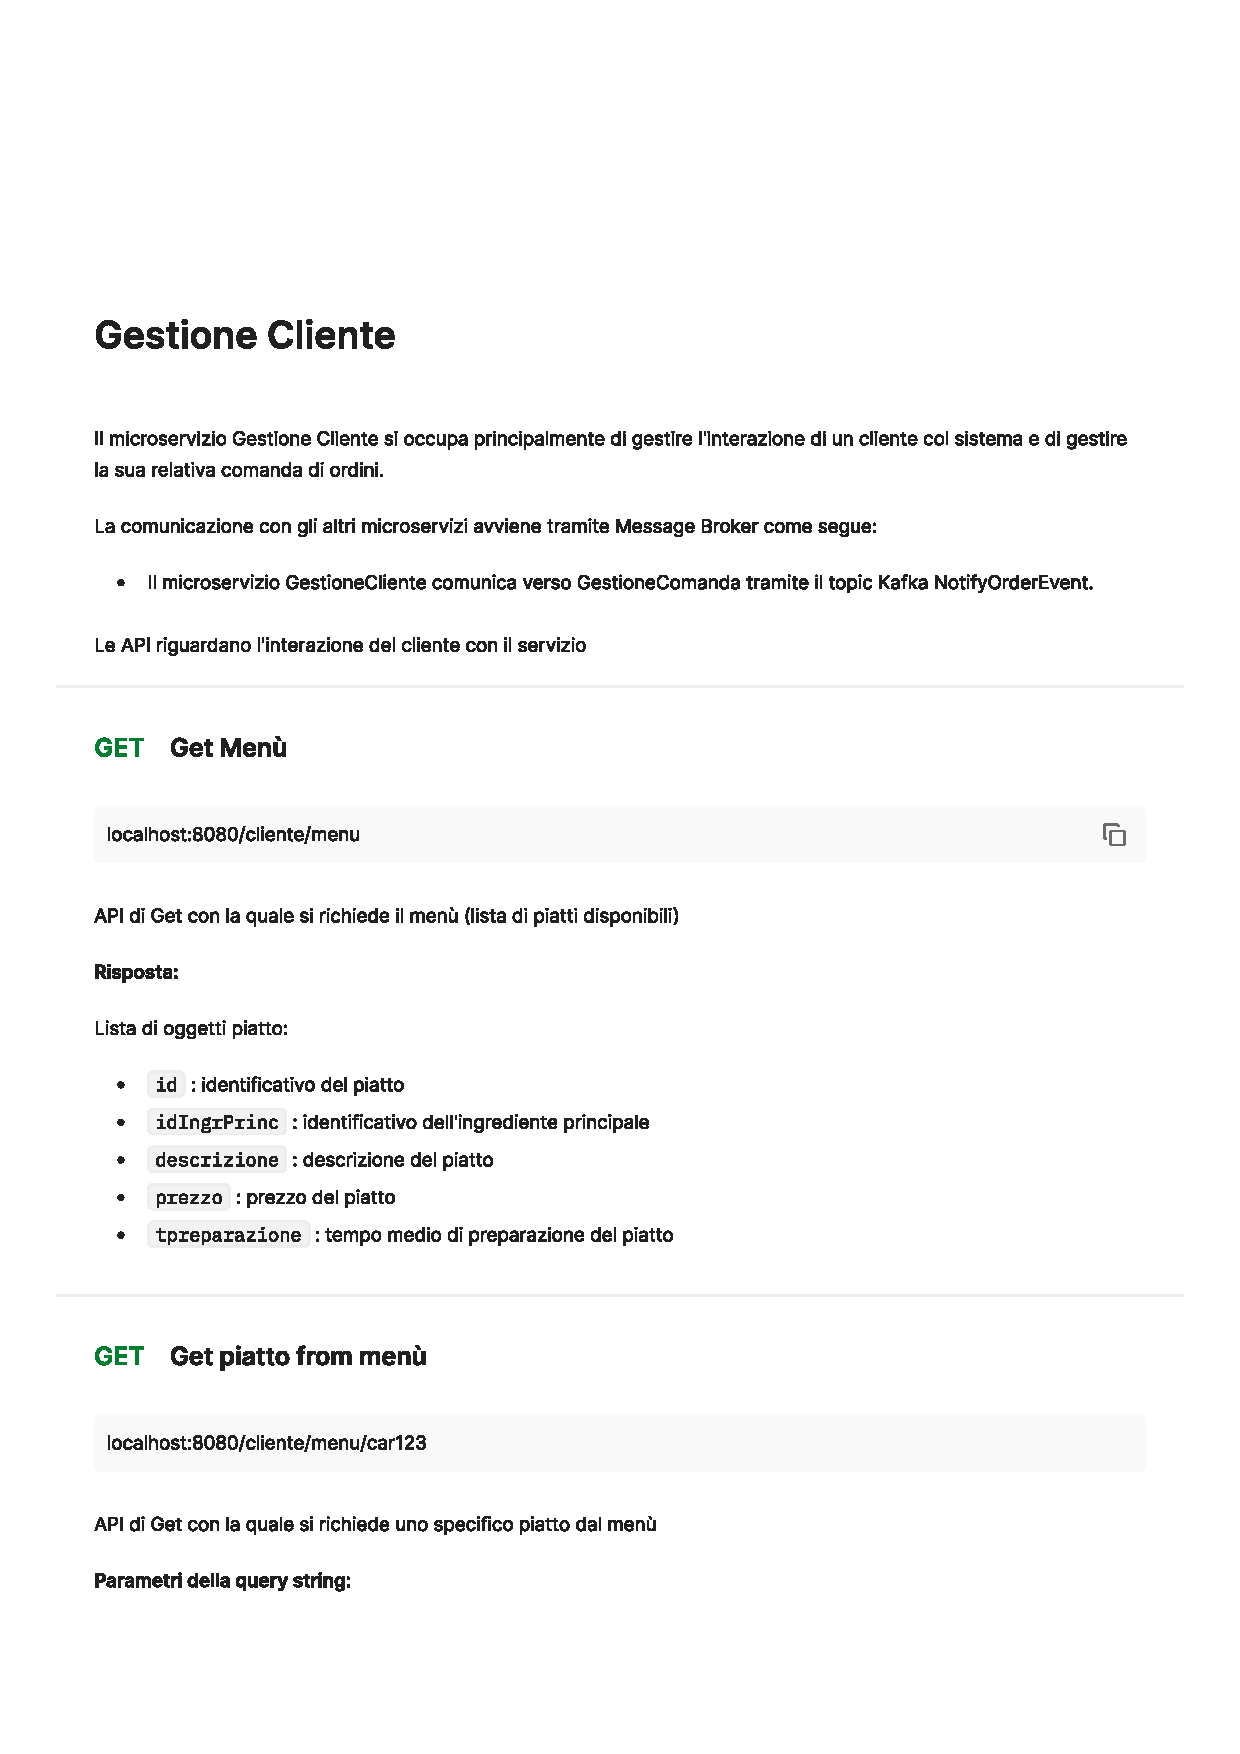
\includepdf[pages=-,pagecommand={\thispagestyle{fancy}},fitpaper=true]{iterazione1/resources/Postman-GestioneCliente.pdf}

%\subsection{API di Gestione Cucina}
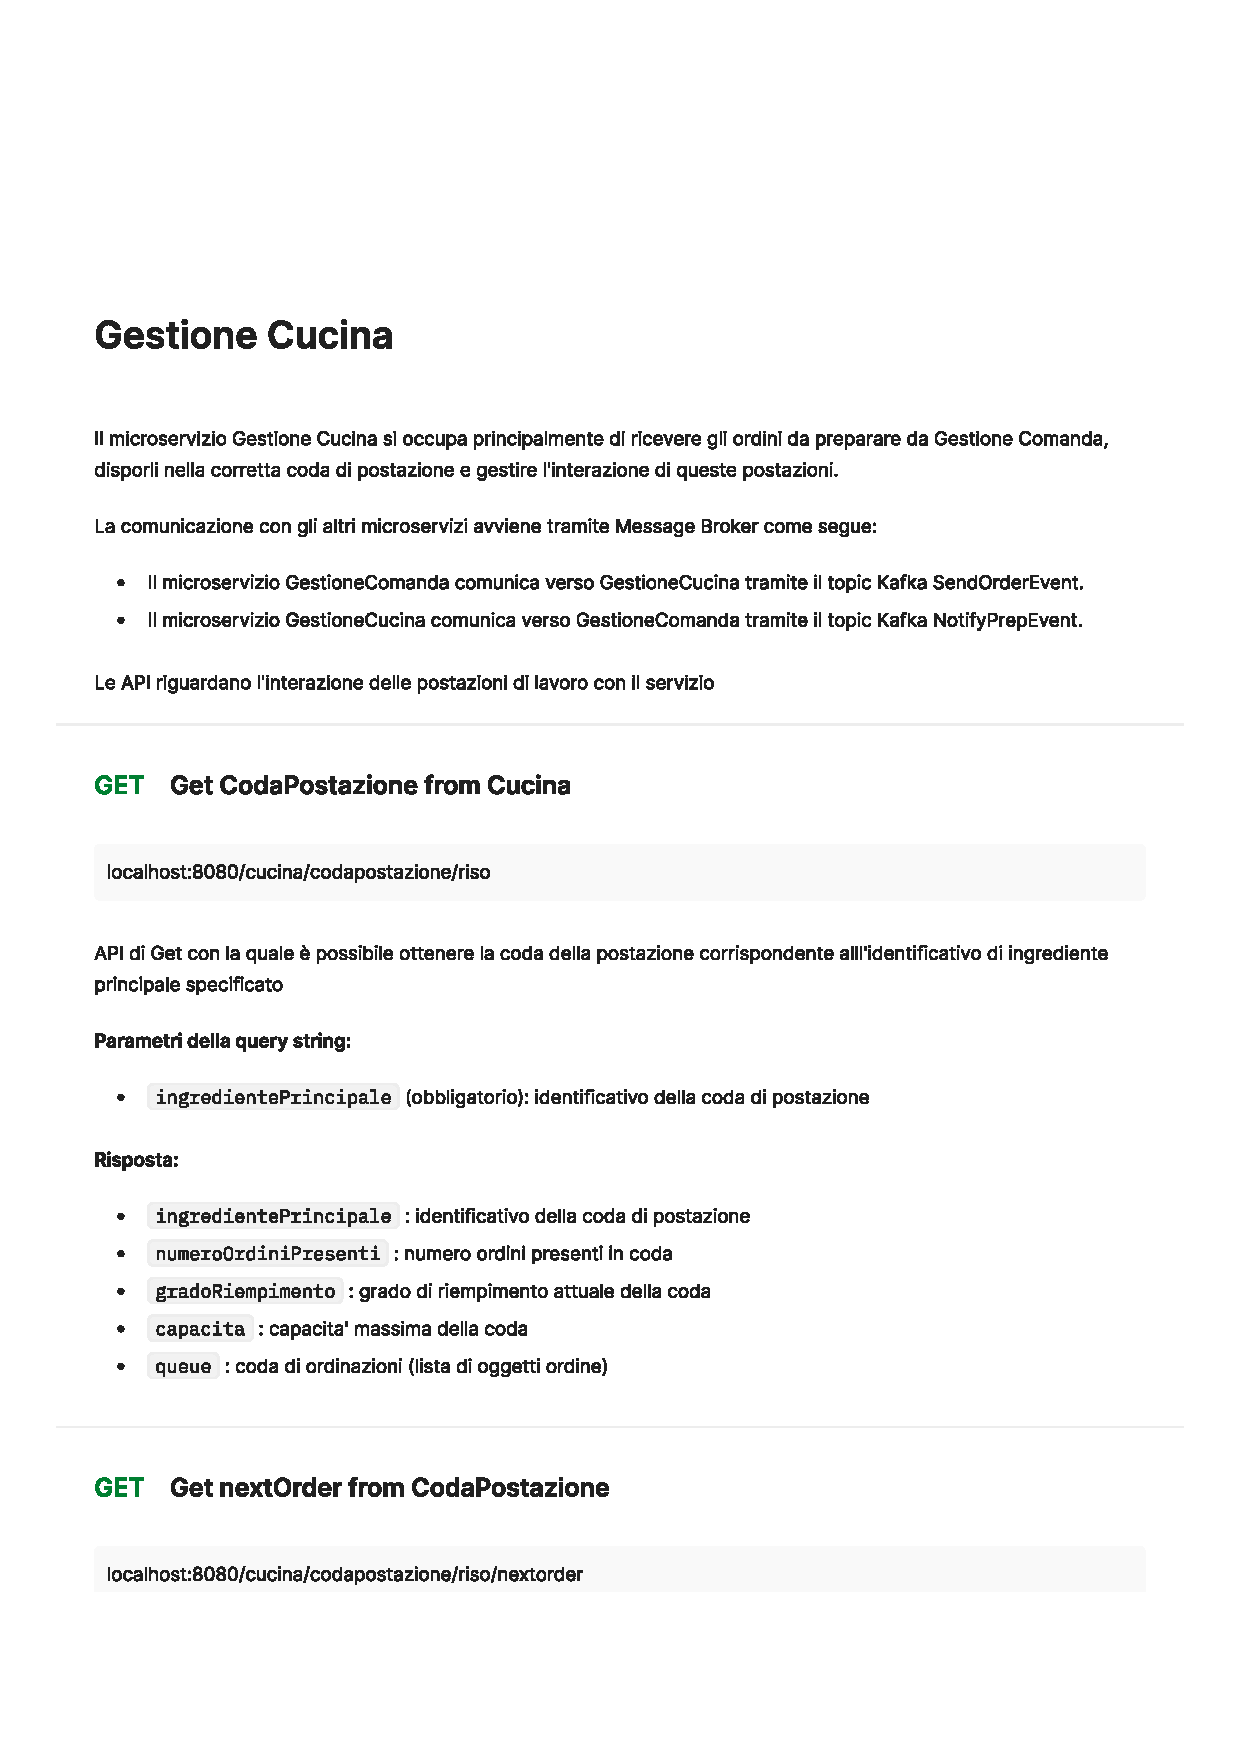
\includepdf[pages=-,pagecommand={\thispagestyle{fancy}},fitpaper=true]{iterazione1/resources/Postman-GestioneCucina.pdf}

\clearpage
    \section{Analisi statica CheckStyle}

\subsection{Introduzione}

Garantire la qualità del codice sorgente è fondamentale per assicurare la stabilità, l'affidabilità e la manutenibilità delle applicazioni. Tra gli strumenti utilizzati per questo scopo, l'analisi statica del codice riveste un ruolo cruciale. In questo Progetto è quindi stato utilizzato \textbf{Checkstyle}, \href{https://checkstyle.sourceforge.io/}{https://checkstyle.sourceforge.io/}, che permette una valutazione automatica della conformità del codice e linee guida da seguire.
\\
Questo documento si propone di fornire una panoramica dettagliata sull'utilizzo di Checkstyle per condurre analisi statiche del codice sorgente. Esploreremo le sue funzionalità, le principali regole di analisi implementate e i benefici derivanti dall'integrazione di questa pratica nella fase di sviluppo del software. Vengono ora mostrati alcuni report generati dai vari microservizi.


È inoltre possibile visualizzare per intero i report generati nei seguenti documenti:


\begin{itemize}
	\item Gestione Comanda: 
	
	{\small 	\href{https://giorgio-hash.github.io/ServeEasy/Report/GestioneComanda/site/checkstyle.html}{https://giorgio-hash.github.io/ServeEasy/Report/GestioneComanda/site/checkstyle.html}}
	\item Gestione Cliente: 
	
	{\small 	\href{https://giorgio-hash.github.io/ServeEasy/Report/GestioneCliente/site/checkstyle.html}{https://giorgio-hash.github.io/ServeEasy/Report/GestioneCliente/site/checkstyle.html}}
	\item Gestione Cucina: 
	
	{\small \href{https://giorgio-hash.github.io/ServeEasy/Report/GestioneCucina/site/checkstyle.html}{https://giorgio-hash.github.io/ServeEasy/Report/GestioneCucina/site/checkstyle.html}}
\end{itemize}
Per poter visualizzare i file di report online si è utilizzato il servizio offerto da GitHub: GitHub Pages\cite{github-pages}, esso permette di ospitare siti web statici generati da repository GitHub pubbliche.

\newpage

\subsection{Report Gestione Comanda}

\begin{figure}[htbp]
	\centering
	\includegraphics[scale=0.6]{iterazione1/images/Cs_Summary_Gestione_Comanda.jpg}
	\caption{Sommario di gestione comanda\label{fig:Cs_Summary_Gestione_Comanda}}
\end{figure}

\begin{figure}[htbp]
	\centering
	\includegraphics[scale=0.8]{iterazione1/images/Cs_rules_Gestione_Comanda.jpg}
	\caption{Rules generate da gestione comanda\label{fig:Cs_Rules_Gestione_Comanda}}
\end{figure}

\begin{figure}[H]
	\centering
	\begin{minipage}[b]{1\textwidth}
		\centering
		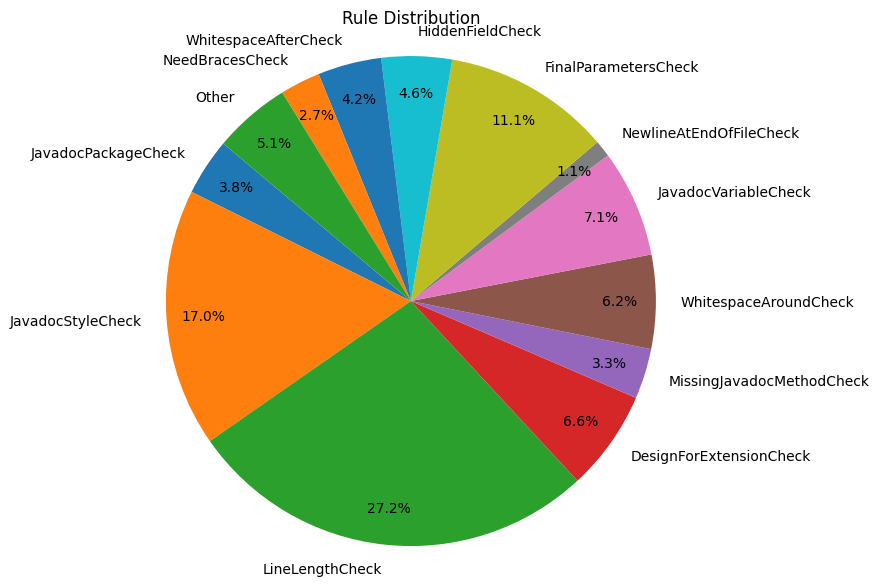
\includegraphics[width=\textwidth]{iterazione1/images/comanda-error_distribution_pie_chart.png}
		\caption{Grafico di tutte le regole}
		\label{fig:comanda-error_distribution_pie_chart}
	\end{minipage}
	\hfill
	\begin{minipage}[b]{0.45\textwidth}
		\centering
		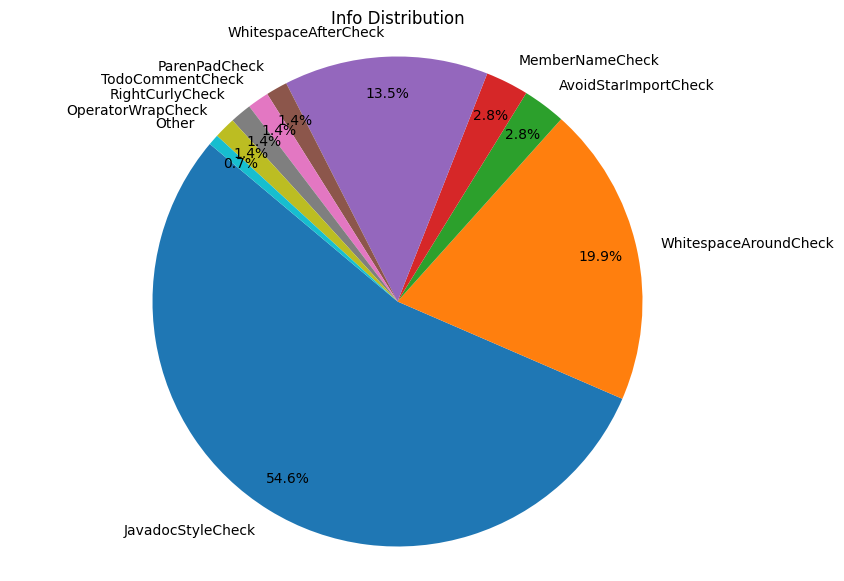
\includegraphics[width=\textwidth]{iterazione1/images/comanda-info_severity_distribution_pie_chart.png}
		\caption{Grafico delle info}
		\label{fig:comanda-info_severity_distribution_pie_chart}
	\end{minipage}
	\vspace{0.5cm}
	\begin{minipage}[b]{0.45\textwidth}
		\centering
		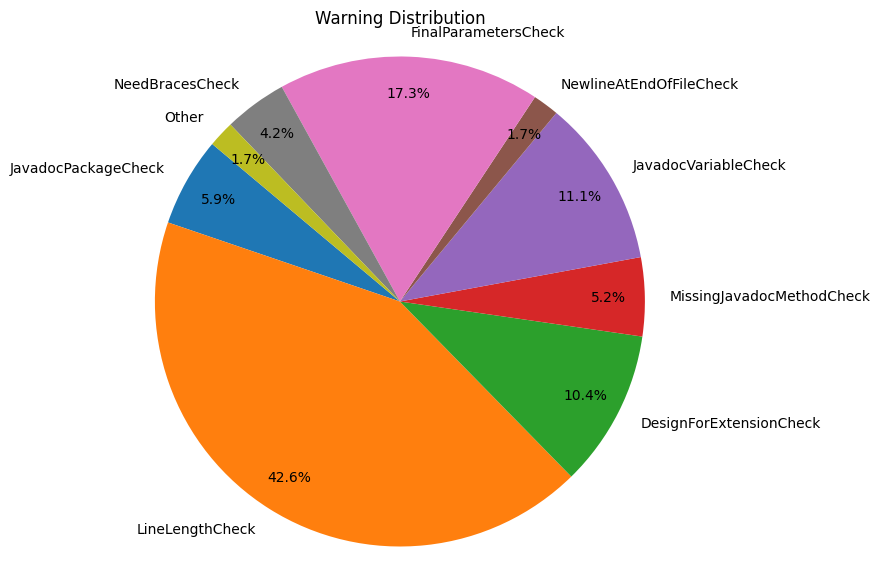
\includegraphics[width=\textwidth]{iterazione1/images/comanda-warning_severity_distribution_pie_chart.png}
		\caption{Grafico degli warnings}
		\label{fig:comanda-warning_severity_distribution_pie_chart}
	\end{minipage}
	\hfill
	\begin{minipage}[b]{0.45\textwidth}
		\centering
		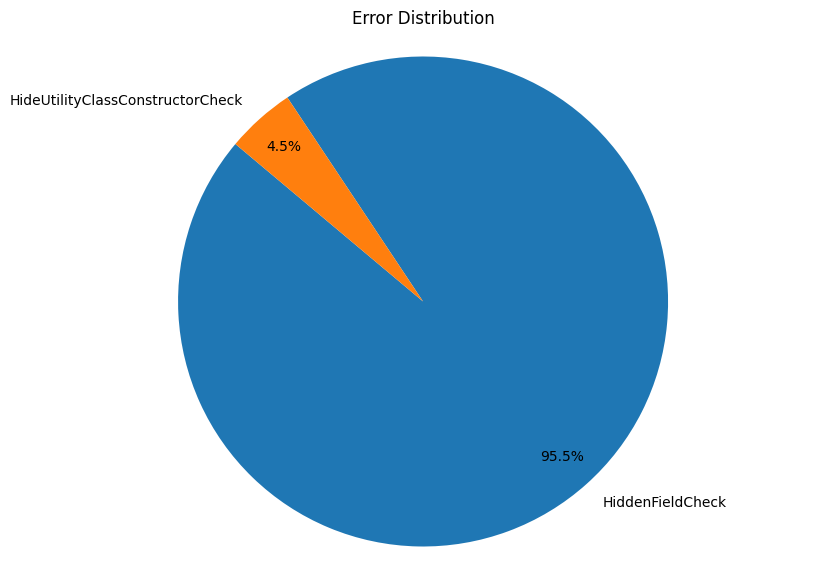
\includegraphics[width=\textwidth]{iterazione1/images/comanda-error_severity_distribution_pie_chart.png}
		\caption{Grafico degli errori}
		\label{fig:comanda-error_severity_distribution_pie_chart}
	\end{minipage}
\end{figure}

\newpage

\subsection{Report Gestione Cliente}

\begin{figure}[htbp]
	\centering
	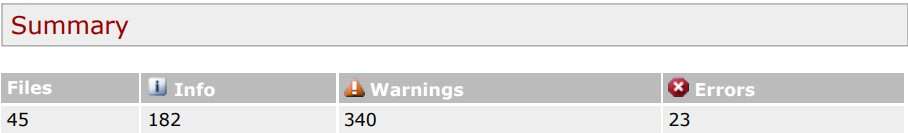
\includegraphics[scale=0.6]{iterazione1/images/Cs_Summary_Gestione_Cliente.jpg}
	\caption{Sommario di gestione cliente\label{fig:Cs_Summary_Gestione_Cliente}}
\end{figure}

\begin{figure}[htbp]
	\centering
	\includegraphics[scale=0.8]{iterazione1/images/Cs_rules_Gestione_Cliente.jpg}
	\caption{Rules generate da gestione cliente\label{fig:Cs_Rules_Gestione_Cliente}}
\end{figure}

\begin{figure}[H]
	\centering
	\begin{minipage}[b]{1\textwidth}
		\centering
		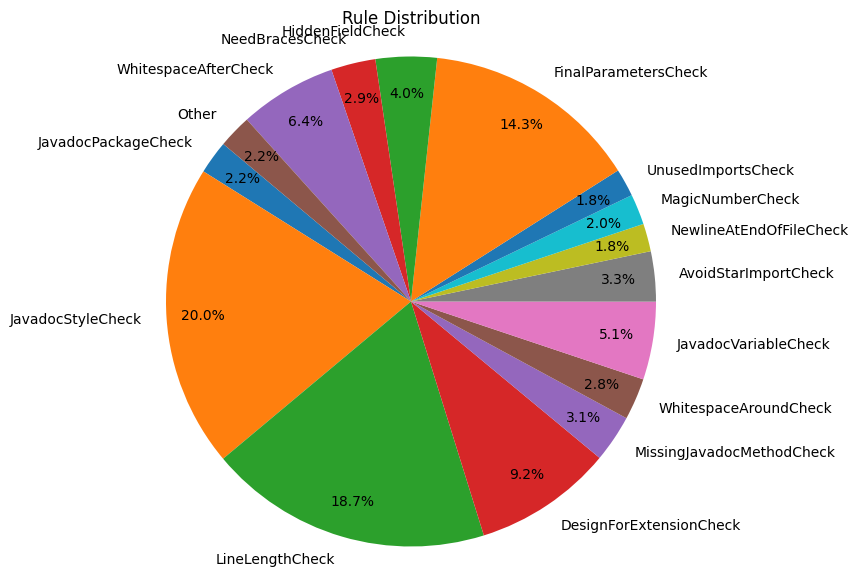
\includegraphics[width=\textwidth]{iterazione1/images/cliente-error_distribution_pie_chart.png}
		\caption{Grafico di tutte le regole}
		\label{fig:cliente-error_distribution_pie_chart}
	\end{minipage}
	\hfill
	\begin{minipage}[b]{0.45\textwidth}
		\centering
		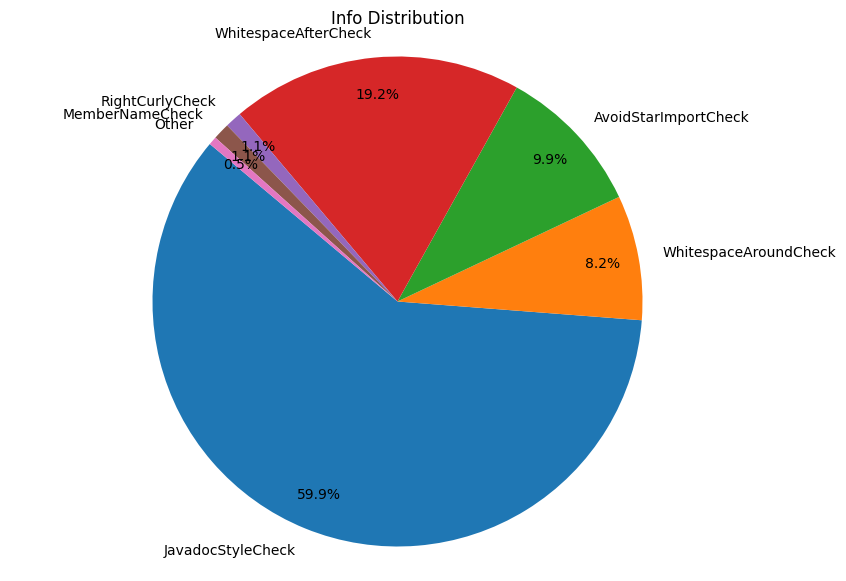
\includegraphics[width=\textwidth]{iterazione1/images/cliente-info_severity_distribution_pie_chart.png}
		\caption{Grafico delle info}
		\label{fig:cliente-info_severity_distribution_pie_chart}
	\end{minipage}
	\vspace{0.5cm}
	\begin{minipage}[b]{0.45\textwidth}
		\centering
		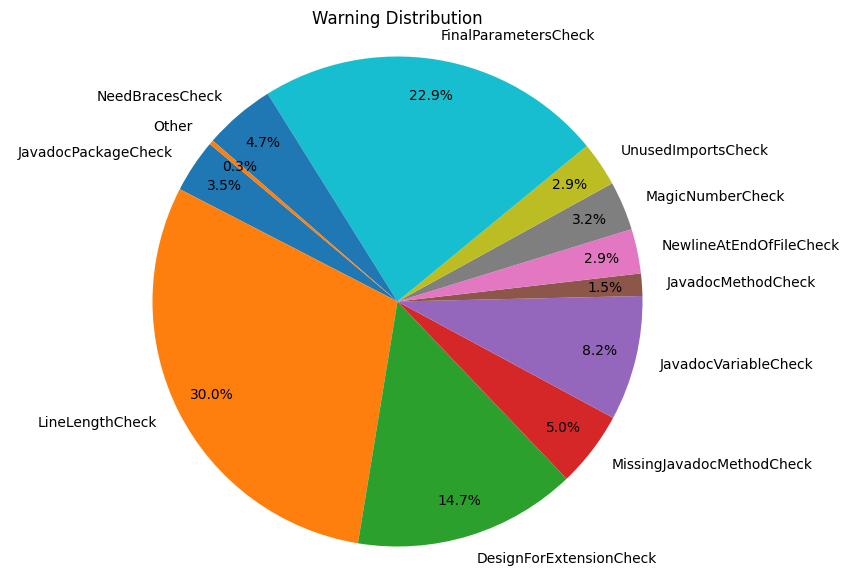
\includegraphics[width=\textwidth]{iterazione1/images/cliente-warning_severity_distribution_pie_chart.png}
		\caption{Grafico degli warnings}
		\label{fig:cliente-warning_severity_distribution_pie_chart}
	\end{minipage}
	\hfill
	\begin{minipage}[b]{0.45\textwidth}
		\centering
		\includegraphics[width=\textwidth]{iterazione1/images/cliente-error_severity_distribution_pie_chart.png}
		\caption{Grafico degli errori}
		\label{fig:cliente-error_severity_distribution_pie_chart}
	\end{minipage}
\end{figure}

\newpage

\subsection{Report Gestione Cucina}

\begin{figure}[htbp]
	\centering
	\includegraphics[scale=0.6]{iterazione1/images/Cs_Summary_Gestione_Cucina.jpg}
	\caption{Sommario di gestione cucina\label{fig:Cs_Summary_Gestione_Cucina}}
\end{figure}

\begin{figure}[htbp]
	\centering
	\includegraphics[scale=0.9]{iterazione1/images/Cs_rules_Gestione_Cucina.jpg}
	\caption{Rules generate da gestione cucina\label{fig:Cs_Rules_Gestione_Cucina}}
\end{figure}

\begin{figure}[H]
	\centering
	\begin{minipage}[b]{1\textwidth}
		\centering
		\includegraphics[width=\textwidth]{iterazione1/images/cucina-error_distribution_pie_chart.png}
		\caption{Grafico di tutte le regole}
		\label{fig:cucina-error_distribution_pie_chart}
	\end{minipage}
	\hfill
	\begin{minipage}[b]{0.45\textwidth}
		\centering
		\includegraphics[width=\textwidth]{iterazione1/images/cucina-info_severity_distribution_pie_chart.png}
		\caption{Grafico delle info}
		\label{fig:cucina-info_severity_distribution_pie_chart}
	\end{minipage}
	\vspace{0.5cm}
	\begin{minipage}[b]{0.45\textwidth}
		\centering
		\includegraphics[width=\textwidth]{iterazione1/images/cucina-warning_severity_distribution_pie_chart.png}
		\caption{Grafico degli warnings}
		\label{fig:cucina-warning_severity_distribution_pie_chart}
	\end{minipage}
	\hfill
	\begin{minipage}[b]{0.45\textwidth}
		\centering
		\includegraphics[width=\textwidth]{iterazione1/images/cucina-error_severity_distribution_pie_chart.png}
		\caption{Grafico degli errori}
		\label{fig:cucina-error_severity_distribution_pie_chart}
	\end{minipage}
\end{figure}


\newpage

\subsection{Specifica}
Di seguito vengono ora date le Specifiche segnalate dai vari report.

\paragraph{Errors:}

	\begin{itemize}

		\item La regola \textbf{\textbf{HiddenField}} controlla se una variabile locale o un parametro ha lo stesso nome di un campo \text{(field)} definito nella stessa classe.

		\item La regola \textbf{\textbf{hideUtilityClassConstructor}} si assicura che le classi di tilità non abbiano un costruttore pubblico. Le classi di utilità sono spesso utilizzate per raggruppare funzionalità comuni e non dovrebbero essereistanziate direttamente. Pertanto, i costruttori di queste classi dovrebbero essere privati o, se si desidera consentire l’ereditarietà, protetti.

	\end{itemize}

\paragraph{Warning:}

	\begin{itemize}

		\item La regola \textbf{\textbf{NeedBraces}} controlla se i blocchi di codice \text{(if, else, for, while, ecc.)} sono racchiusi tra parentesi graffe.

		\item La regola \textbf{\textbf{MagicNumber}} controlla se ci sono numeri letterali nel codice che non sono definiti come costanti. In altre parole, i“magic numbers” sono valori numerici che compaiono direttamente nel codice senza essere assegnati a una variabile o costante.

		\item La regola \textbf{\textbf{designForExtension}} controlla se le classi sono progettate per essere estese tramite sottoclassi. È particolarmente utile nei progetti di librerie (non nei progetti di applicazioni) che si preoccupano di seguire un design OOP ideale per garantire che le classi funzionino correttamente in tutti i casi, anche in caso di uso improprio.

		\item La regola \textbf{\textbf{UnusedImports}} verifica gli import nonutilizzati all’interno del codice.

		\item La regola \textbf{\textbf{JavadocMethod}} controlla la documentazione Javadoc di un metodo o di un costruttore.

		\item La regola \textbf{\textbf{JavadocPackage}} verifica che ogni pacchetto Javaabbia un file Javadoc utilizzato per i commenti. Di default, consente solo un file package-info.java, ma può essere configurata per consentire un file “package.html” Verrà segnalata una violazione se entrambi i file esistono,poiché ciò non è consentito dallo strumento Javadoc.

		\item La regola \textbf{\textbf{JavadocVariable}} controlla se una variabile ha uncommento Javadoc. Viene segnalata una violazione se manca il commento Javadoc per qualsiasi membro di visibilità.

		\item La regola \textbf{\textbf{MissingJavadocMethod}} verifica la presenza di commenti Javadoc mancanti per metodi o costruttori.

		\item La regola \textbf{\textbf{FinalParameters}} verifica che i parametri per metodi, costruttori, blocchi catch e blocchi for-each siano dichiarati come final. Tuttavia, i metodi di interfaccia, astratti e nativi non vengono controllati: la parola chiave final non ha senso per i parametri dei metodi di interfaccia, astratti e nativi poiché non esiste alcun codice che potrebbe modificare il parametro.

		\item La regola \textbf{\textbf{NewlineAtEndOfFile}} verifica se i file terminano con un separatore di riga.

		\item La regola \textbf{\textbf{LineLength verifica}} se le righe sono troppo lunghe. Questo è importante perché le righe lunghe possono essere difficili da leggere,specialmente quando si stampa il codice o quando gli sviluppatori hanno uno spazio limitato sullo schermo (ad esempio, se l’IDE mostra altre informazioni come l’albero del progetto o la gerarchia delle classi).

	\end{itemize}

\paragraph{Info:}

	\begin{itemize}

		\item La regola \textbf{\textbf{LeftCurly}} controlla la posizione delle parentesi graffe aperte all’interno dei blocchi di codice.

		\item La regola \textbf{\textbf{RightCurly}} controlla se le parentesi graffe chiuse sono posizionate correttamente all’interno dei blocchi di codice.

		\item La regola \textbf{\textbf{AvoidStarImport}} controlla se ci sono dichiarazioni di importazione che utilizzano l’asterisco *. Importare tutte le classi da un pacchetto o membri statici da una classe porta a un accoppiamento stretto tra pacchetti o classi e potrebbe causare problemi quando una nuovaversione di una libreria introduce conflitti di nomi.

		\item La regola \textbf{\textbf{JavadocStyle}} verifica che i commenti Javadoc siano ben formati. (punteggiatura alla fine della prima frase, verifica della presenza di descrizione, verifica dei tag html incompleti, verifica documentazione del pacchetto, tag html consentiti).

		\item La regola \textbf{\textbf{TodoComment}} verifica la presenza di commenti con la parola chiave “TODO:”. In realtà, è un matcher generico di pattern per i commenti Java. Per verificare altri pattern nei commenti Java, è possibile impostare la proprietà format. L’utilizzo dei commenti “TODO:” è un ottimo modo per tenere traccia dei compiti da svolgere.

		\item La regola \textbf{\textbf{LocalVariableName}} verifica che i nomi delle variabili locali (variabili dichiarate all’interno di un metodo o di un blocco)siano conformi a un pattern specificato.

		\item La regola \textbf{\textbf{MethodParamPad}} controlla la spaziatura tra l’identificatore di una definizione di metodo, una definizione di costruttore,una chiamata di metodo o una chiamata di costruttore e la parentesi sinistra della lista dei parametri.

		\item La regola \textbf{\textbf{NoWhitespaceBefore}}  verifica che non ci sia spazio bianco prima di un token specifico. In particolare, controlla che il token non sia preceduto da spazio bianco

		\item La regola \textbf{\textbf{OperatorWrap}} verifica come gli operatori sono posizionati rispetto alle righe di codice. In particolare, controlla se gli operatori dovrebbero essere posizionati sulla stessa riga o su una nuova riga. Questo è importante per mantenere la leggibilità del codice e per seguire le convenzioni di stile.

		\item La regola \textbf{\textbf{ParenPad}} verifica come le parentesi sono posizionate rispetto alle righe di codice. In particolare, controlla se le parentesi dovrebbero essere seguite da spazio o se devono essere adiacenti senza spazi.

		\item La regola \textbf{\textbf{WhitespaceAfter}} controlla come gli spazi bianchi sono posizionati rispetto ai token nel codice sorgente. In particolare,verifica se gli operatori dovrebbero essere seguiti da spazio o se devono essere adiacenti senza spazi.

		\item La regola \textbf{\textbf{WhitespaceAround}}  verifica che un token sia circondato da spazio bianco. Questa regola si applica a vari contesti, come loop vuoti e lambda vuote.

		\item La regola \textbf{\textbf{redundantModifier}} è progettata per individuare e segnalare i modificatori ridondanti all'interno del codice sorgente Java. Questa regola controlla i modificatori di accesso, come public, protected,private, e anche i modificatori come final, abstract, static e strictfp.

	\end{itemize}

\subsection{Checkstyle}

\paragraph{Installazione:}
Per poter utilizzare le funzionalità di checkstyle all'interno dell'IDEA itelliJ è stato installa un plugin disponibile all'interno del marketplace di IntelliJ, ovvero CheckStyle-IDEA\cite{jetbrains}. Di seguito viene mostrata la schermata che permette l'installazione di quest'ultima.

\begin{figure}[htbp]
	\centering
	\includegraphics[scale=0.8]{iterazione1/images/Install_checkstyle_intelliJ.jpg}
	\caption{Schermata installazione plugin\label{fig:Install_checkstyle_intelliJ}}
\end{figure}

\paragraph{Configurazione e personalizzazione:}
Per la configurazione del plugin di checkstyle in maven è stato introdotto all'interno del file \textbf{pom.xml} la seguente: 

\begin{lstlisting}[language=XML, caption={plugin Maven con Maven Checkstyle Plugin}]
<plugin>
	<groupId>org.apache.maven.plugins</groupId>
	<artifactId>maven-checkstyle-plugin</artifactId>
	<version>3.3.1</version>
	<configuration>
		<configLocation>checkstyle.xml</configLocation>
	</configuration>
	<executions>
		<execution>
			<goals>
				<goal>checkstyle</goal>
			</goals>
		</execution>
	</executions>
</plugin>
\end{lstlisting}

Abbiamo quindi creato un file Checkstyle.xml personalizzando le regole di Sun Checkstyle, che definiscono un insieme di regole di programmazione per la scrittura del codice. Questo ci aiuta a adattare le regole alle nostre specifiche esigenze, garantendo uno stile di codifica coerente e di alta qualità. Le categorie di violazioni controllate sono: Blocks, coding, design, javadoc, imports, misc, naming, sizes, whitespace e modifier.

\begin{lstlisting}[language=XML, caption={Personalizzazioni regole di Sun Checkstyle}]
<?xml version="1.0"?>
<!DOCTYPE module PUBLIC
        "-//Checkstyle//DTD Checkstyle Configuration 1.3//EN"
        "https://checkstyle.org/dtds/configuration_1_3.dtd">

<!--
  Checkstyle configuration that checks the sun coding
-->

<module name="Checker">

    <property name="severity" value="error"/>

    <property name="fileExtensions" value="java, properties, xml"/>

    <!-- Excludes all 'module-info.java' files              -->
    <module name="BeforeExecutionExclusionFileFilter">
        <property name="fileNamePattern" value="module\-info\.java$"/>
    </module>

    <module name="SuppressionFilter">
        <property name="file" value="${org.checkstyle.sun.suppressionfilter.config}"
                  default="checkstyle-suppressions.xml" />
        <property name="optional" value="true"/>
    </module>

    <!-- Checks that a package-info.java file exists for each package.     -->
    <module name="JavadocPackage">
        <property name="severity" value="warning"/>
    </module>

    <!-- Checks whether files end with a new line.                        -->
    <module name="NewlineAtEndOfFile">
        <property name="severity" value="warning"/>
    </module>

    <!-- Checks that property files contain the same keys.         -->
    <module name="Translation"/>

    <!-- Checks for Size Violations.                    -->
    <module name="FileLength">
        <property name="severity" value="warning"/>
    </module>
    <module name="LineLength">
        <property name="fileExtensions" value="java"/>
        <property name="severity" value="warning"/>
    </module>

    <!-- Checks for whitespace                               -->
    <module name="FileTabCharacter">
        <property name="severity" value="warning"/>
    </module>

    <module name="TreeWalker">

        <!-- Checks for Javadoc comments.                     -->
        <module name="InvalidJavadocPosition">
            <property name="severity" value="warning"/>
        </module>
        <module name="JavadocMethod">
            <property name="severity" value="warning"/>
        </module>
        
        <!-- Checks for Naming Conventions.                  -->
        <module name="ConstantName">
            <property name="severity" value="info"/>
        </module>
        <module name="LocalFinalVariableName">
            <property name="severity" value="info"/>
        
        <!-- Checks for imports                              -->
        <module name="AvoidStarImport">
            <property name="severity" value="info"/>
        </module>
        <module name="IllegalImport"> 

        <!-- Checks for Size Violations.                    -->
        <module name="MethodLength">
            <property name="severity" value="info"/>
        </module>
        <module name="ParameterNumber">
            <property name="severity" value="info"/>
        </module>

        <!-- Checks for whitespace                               -->
        <module name="EmptyForIteratorPad">
            <property name="severity" value="info"/>
        </module>
        <module name="GenericWhitespace">
            <property name="severity" value="info"/>
        </module>

        <!-- Checks for blocks. You know, those {}'s         -->
        <module name="AvoidNestedBlocks">
            <property name="severity" value="warning"/>
        </module>
        <module name="EmptyBlock">
            <property name="severity" value="error"/>
        </module>

        <!-- Checks for class design                         -->
        <module name="DesignForExtension">
            <property name="severity" value="warning"/>
        </module>
        <module name="FinalClass">
            <property name="severity" value="warning"/>
        </module>


        <module name="SuppressionXpathFilter">
            <property name="file" value="${org.checkstyle.sun.suppressionxpathfilter.config}"
                      default="checkstyle-xpath-suppressions.xml" />
            <property name="optional" value="true"/>
        </module>

    </module>

</module>
\end{lstlisting}

\paragraph{Esecuzione:}
Avvenuta la fase di installazione e configurazione è ora possibile identificare e correggere le violazioni di stile definite nel file di configurazione.

Per eseguire il controllo di stile è sufficiente eseguire il comando:
\begin{lstlisting}[style=terminal, 
	caption={Avvio controllo checkstyle}]
mvn site
\end{lstlisting}

Esso permetterà di generare all'interno della directory \textbf{target > site} contenente i file html e xml con i report generati.



\subsection{Generazione Grafi}
Al fine di poter visualizzare con più semplicità i file di report sono stati generati dei grafici a torta che mostrano il tipo di errore rilevato e la percentuale delle volte in cui è stato commesso.
Per creare questi grafici abbiamo creato un semplice script python da allegare al progetto di ogni microservizio. 
\subsubsection{Script Python}
Questo script si basa sul file "checkstyle-result.xml" generato dal report di checkstyle e posizionato nella cartella target, quindi come prima cosa viene caricato questo file:
\begin{lstlisting}[style=pythonstyle, caption={Script Python - aggiunta checkstyle-result.xml}, label=lst:python-checkstyle-result]
script_dir = os.path.dirname(os.path.abspath(__file__))
input_xml_file = 
	os.path.join(script_dir, "target", "checkstyle-result.xml")
\end{lstlisting}
Successivamente si passa a fare il parsing di questo file, andando a scandire i vari elementi <error> per ogni singolo <file>, in particoalre si classificano gli errori in base all'attributo severity che può essere info, warning ed error. In questo modo si creano 3 dizionari con questi tipi di valore di severità, oltre a un altro globale che contiene la somma di tutti e 3 gli errori chiamato rule, ed ad ogni occorrenza di un errore data dall'attributo source di error si aumenta il conteggio del dizionario alla chiave corrispondente a quel attributo. Come mostrato da questo pezzo di codice:
\begin{lstlisting}[style=pythonstyle, caption={Script Python - parsing checkstyle-result.xml}, label=lst:python-parsing]
tree = Et.parse(xml_file)
root = tree.getroot()
error_counts = defaultdict(int)
for file in root.findall('file'):
	for error in file.findall('error'):
		if error.get('severity') == severity or skip is True:
			source = error.get('source')
			error_counts[error_type] += 1
\end{lstlisting}
Successivamente si passa a convertire ogni dizionario in un file csv, il quale sarà costruito in modo tale da avere come prima colonna il tipo di errore e come seconda il numero di volte che è stato commesso quell'errore.
Nel passo successivo questi file csv vengono convertiti in un grafico a torta utilizzando la libreria matplotlib.pyplot e salvati in un file png.
\begin{lstlisting}[style=pythonstyle, caption={Script Python - Plot pie chart}, label=lst:python-piechart]
errors = list(error_counts.keys())
counts = list(error_counts.values())
[...]
plt.figure(figsize=(10, 7))
patches, texts, _ = plt.pie(counts, labels=errors, autopct='%1.1f%%', startangle=140, pctdistance=0.85)
plt.axis('equal')
plt.title(title + " Distribution")
plt.savefig(output_file, bbox_inches='tight')
\end{lstlisting}
I file csv e le immagini png vengono salvati nella cartella di percorso target/output/csv per i primi, mentre target/output/images per le seconde.
\paragraph{Come avviarlo:}
per poter avviare lo script python è necessario avere Python installato sul proprio PC\cite{phoenixnap} ed eseguire il seguente comando per installare le librerie necessarie:
\begin{lstlisting}[style=terminal, 
	caption={Python - installare i pacchetti necessari}, label=lst:python-pip-install]
pip install -r python/requirements.txt
\end{lstlisting}
Successivamente eseguire il seguente per poter avviare lo script:
\begin{lstlisting}[style=terminal, 
	caption={Avvio script python}, label=lst:python-main]
python main.py
\end{lstlisting}
È possibile trovare i file generati in target/output dalla root del progetto.
\paragraph{Output:}
esempio di file csv in output:
\begin{lstlisting}[style=pythonstyle, caption={file checkstyle\_warning\_severity\_counts.csv warning di gestione comanda}, label=lst:csv-warning]
Warning,Count
JavadocPackageCheck,17
LineLengthCheck,123
DesignForExtensionCheck,30
MissingJavadocMethodCheck,15
UnusedImportsCheck,2
JavadocVariableCheck,32
JavadocMethodCheck,2
NewlineAtEndOfFileCheck,5
MagicNumberCheck,1
FinalParametersCheck,50
NeedBracesCheck,12
\end{lstlisting}
Grafico a torta associato:
\begin{figure}[htbp]
	\centering
	\includegraphics[scale=0.6]{iterazione1/images/warning_severity_distribution_pie_chart.png}
	\caption{Grafico warnings di gestione comanda\label{fig:graph_warning_gestionecomanda}}
\end{figure}

\clearpage
    \section{Analisi statica SonarQube}
A causa della mancanza di ulteriori analisi all'interno del plugIn di Checkstyle è stata inserito un ulteriore strumento, ovvero SonaQube \cite{SonarQube}.

Esso è uno strumento che consente ad un team di scrivere codice più pulito e più sicuro. Esso garantisce un'ispezione continua del codice e mette a disposizione migliaia di regole automatizzate finalizzate all’analisi statica del codice. Queste regole forniscono protezione al progetto esaminato e guidano il team di sviluppo.

La home page dello strumento fornisce una fotografia della situazione, in termini di qualità, del progetto sottoposto all’analisi.

Tramite la pagina Issues è possibile valutare in dettaglio ogni problematica trovata, quali sono le issue principali, dove si trovano nel codice e quando sono stati aggiunti.
Per ciascun dominio SonarQube fornisce un diagramma a bolle che mette in correlazione diverse metriche.


\subsection{SonarQube}
\paragraph{Creazione Container SonarQube:}
Per poter utilizzare le funzionalità di sonarqube all'interno del nostro progetto è stato scelto l'implementazione attraverso offerta dal framework Docker, dove viene garantito un ambiente altamente personalizzabile, flessibile e di facile implementazione all'interno di ogni container.
Una volta istanziati i volumi di Docker e modificato il $docker-compose.yaml$, la localhost utilizzata dal componente di sonarqube sarà la porta \textbf{9000}.

\paragraph{Installazione:}
Creati i volumi sono stati inseriti all'interno del $pom.xml$ di maven i seguenti plugin.

\begin{lstlisting}[language=XML, caption={Implementazioni pom.xml}]
<pluginManagement>
    <plugins>
        <plugin>
            <!-- SonarQube -->
            <groupId>org.sonarsource.scanner.maven</groupId>
            <artifactId>sonar-maven-plugin</artifactId>
            <version>3.4.0.905</version>
        </plugin>
    </plugins>
</pluginManagement>
\end{lstlisting}

Come si può notare è stato necessario inserire anche \textbf{Jacoco}\cite{Jacoco}, \textbf{PMD}\cite{PMD} e \textbf{SpotBugs}\cites{spotbugs} come plugin maven, ovvero una copertura di codice che misura la qualità di un programma che è stato effettivamente eseguito durante un test, così da determinare se il codice è stato testato in modo completo ed efficace.

\paragraph{Come usare SonarQube:}

Una voltà fatto partire il cointainer contenente SonarQube sarà necessario:

\begin{itemize}
 \item accedere all'interfaccia localhost:9000;
 \item inserire user e pasword iniziali (username: admin / password: admin);
 \item modicare la propria password con una propria locale;
 \item creare un nuovo progetto locale impostando nomi e branch desiderati;
 \item generare un \textbf{token} locale e specificare mavem come proprio framework;
 \item lanciare su cmd (non usare PowerShell) il proprio comando:
\begin{lstlisting}[style=terminal, 
	caption={Avvio sonarqube}]
    .\mvnw clean verify site spotbugs:spotbugs sonar:sonar -Dsonar.projectKey=GestioneComanda -Dsonar.projectName='GestioneComanda' -Dsonar.host.url=http://localhost:9000 -Dsonar.token=INSERIRE_PROPRIO_TOKEN_SONARQUBE -Dsonar.java.pmd.reportPaths=/target/pmd.xml -Dsonar.java.checkstyle.reportPaths=/target/checkstyle-result.xml -Dsonar.java.spotbugs.reportPaths=/target/spotbugsXml.xml
\end{lstlisting}
\item attendere il fine compilazione e ricaricare la pagina localohost:9000.
\end{itemize}

\subsection{Analisi report SonarQube}
Mostriamo ora significative parti del report generato su alcuni dei nostri microservizi.

\begin{figure}[htbp]
	\centering
	\includegraphics[scale=0.50]{iterazione1/images/Analisys_list_gestione_comanda.png}
	\caption{Analisys list gestione comanda\label{fig:Analisys list gestione comanda}}
\end{figure}

Nella specifica questi controlli servono per:
\begin{itemize}
    \item \textbf{Security (Sicurezza)}:
    \begin{itemize}
        \item La sicurezza del software riguarda la protezione contro le minacce esterne e interne, come hacking, malware e accessi non autorizzati.
        \item Include pratiche come la gestione delle vulnerabilità, l'implementazione di misure di protezione e l'esecuzione di test di sicurezza (penetration testing, security scans).
    \end{itemize}
    \item \textbf{Reliability (Affidabilità)}:
    \begin{itemize}
        \item L'affidabilità del software si riferisce alla capacità del software di funzionare correttamente e senza errori per un periodo di tempo specificato.
        \item Include la gestione degli errori, la ridondanza e la capacità del sistema di recuperare da fallimenti (fault tolerance).
    \end{itemize}
    \item \textbf{Maintainability (Manutenibilità)}:
    \begin{itemize}
        \item La manutenibilità si riferisce alla facilità con cui il software può essere modificato per correggere errori, migliorare le prestazioni o adattarsi a nuovi requisiti.
        \item Comprende aspetti come la leggibilità del codice, la modularità, la documentazione e l'aderenza a standard di codifica.
    \end{itemize}
    \item \textbf{Hotspots Reviewed (Revisioni dei Punti Caldi)}:
    \begin{itemize}
        \item I "punti caldi" sono parti del codice che sono frequentemente modificate o che presentano problemi ricorrenti.
        \item La revisione dei punti caldi implica l'analisi e l'ottimizzazione di queste aree critiche per migliorare la qualità del codice e ridurre il rischio di problemi futuri.
    \end{itemize}
    \item \textbf{Coverage (Copertura)}:
    \begin{itemize}
        \item La copertura del codice si riferisce alla percentuale di codice che viene eseguito durante i test.
        \item Include metriche come la copertura delle linee, delle funzioni e delle condizioni, aiutando a identificare le parti del codice che non sono state testate.
    \end{itemize}
    \item \textbf{Duplications (Duplicazioni)}:
    \begin{itemize}
        \item Le duplicazioni si riferiscono alla presenza di codice duplicato all'interno del progetto software.
        \item Il codice duplicato può aumentare il rischio di errori e rendere il mantenimento più difficile. Rimuovere le duplicazioni aiuta a mantenere il codice più pulito e manutenibile.
    \end{itemize}
\end{itemize}

\newpage
Alcune immagini create per mostrare i test di sonarqube che permettono di individuare le parti di maggior interesse.
Esse Vengono rappresentate anche attraverso grafici di bole facilmente leggibili e interattivi.

\begin{figure}[htbp]
	\centering
	\includegraphics[scale=0.35]{iterazione1/images/coverage_percent_modifier.png}
	\caption{Coverage variata nel corso delle modifiche testate\label{fig:coverage percent modifier}}
\end{figure}

\begin{figure}[htbp]
	\centering
	\includegraphics[scale=0.50]{iterazione1/images/secutiry.png}
	\caption{diagramma di Bolle sulla secutity\label{fig:security}}
\end{figure}

\begin{figure}[htbp]
	\centering
	\includegraphics[scale=0.50]{iterazione1/images/risk.png}
	\caption{diagramma di Bolle sui risk\label{fig:risk}}
\end{figure}

\begin{figure}[htbp]
	\centering
	\includegraphics[scale=0.50]{iterazione1/images/issues.png}
	\caption{overview issues\label{fig:issues}}
\end{figure}

\begin{figure}[htbp]
	\centering
	\includegraphics[scale=0.50]{iterazione1/images/visione_issue.png}
	\caption{issues specifico\label{fig:visione issues}}
\end{figure}

\begin{figure}[htbp]
	\centering
	\includegraphics[scale=0.50]{iterazione1/images/esempio_issue.png}
	\caption{view singolo issue\label{fig:esempio issue}}
\end{figure}

\begin{figure}[htbp]
	\centering
	\includegraphics[scale=0.40]{iterazione1/images/gestione_cucina_overview.png}
	\caption{gestione cucina overview\label{fig:gestione cucina overview}}
\end{figure}

\begin{figure}[htbp]
	\centering
	\includegraphics[scale=0.60]{iterazione1/images/esempio_caso_uncoverage.png}
	\caption{esempio caso uncoverage\label{fig:esempio caso uncoverage}}
\end{figure}

\newpage
Una breve Panoramica delle rules di java esistenti su SonarQube, ognuna di esse può essere totalmente modificata.
\begin{figure}[htbp]
	\centering
	\includegraphics[scale=0.30]{iterazione1/images/java_rules.png}
	\caption{java rules overview sonarqube\label{fig:java rules}}
\end{figure}

\clearpage
    \chapter{Iterazione 2}
    \section{Introduzione}
Nella Iterazione 2 ci si è focalizzati a studiare l'algoritmo più adatto per la nostra applicazione, partendo dall'organizzare le entità interessate, passando poi per scrivere lo pseudo-codice ed infine ad analizzare le strutture dati necessarie.

\paragraph{Briefing} Nell'ambito di questa applicazione si considera che ogni piatto sia composto da un ingrediente principale e da più ingredienti secondari.
Ogni piatto ordinato viene chiamato ordine, quindi un ordine comprende un singolo piatto, mentre la comanda contiene tutti gli ordini di un singolo cliente.
Nel corso di un brainstorming, si è maturata l’idea di organizzare la cucina in postazioni, ognuna focalizzata su un ingrediente principale: ogni postazione si occuperà quindi di preparare e completare piatti accomunati dallo stesso ingrediente principale.
\clearpage
    \section{Organizzazione del lavoro}

\subsection{Organizzazione del processo di sviluppo}
Per l’implementazione dei microservizi che compongono il sistema ServeEasy, attualmente delineato al primo zoom-in, è stato applicato un approccio “polyrepo"\cite{polyrepo}, definendo per ogni microservizio un’area di progetto dedicata. 

Scelta GitHub come piattaforma di hosting per il progetto software, un membro del team è stato incaricato del setup, controllo e gestione delle repository per i singoli microservizi.

Per raggiungere tale organizzazione, è stata prima di tutto creata un’area di lavoro per familiarizzare con le tecnologie selezionate, impiegando uno sforzo congiunto nello studio e prototipazione.

Nel processo di sviluppo sono state specificate delle regole mutualmente pattuite:
\begin{itemize}
    \item Nessuno esegue push diretto dall’area di lavoro locale verso il main branch: ognuno lavora esclusivamente sulla propria branch;
    \item Nei commit e nelle pull requests va espressa una sintesi del proprio lavoro svolto;
\item Cambiamenti importanti vanno discussi;
\item Ogni implementazione va testata;
\item Prima di effettuare una merge sul main branch, l’implementazione deve aver passato le fasi di build e di test con successo.
\end{itemize}

A supporto del processo di sviluppo, sono state introdotte automatizzazioni per garantire Continuous Integration e Continuous Delivery, servendosi di Github Workflows e Docker allo scopo di aumentare la velocità di deployment delle nuove modifiche apportate, garantendo al contempo integrità:
\begin{itemize}
    \item Un evento di push verso il proprio branch causa l’avvio della job di CI posta a sorveglianza del proprio spazio di lavoro sulla repository, allo scopo di effettuare un controllo di compilazione;
    \item Un evento verso il main branch (quale, ad esempio, una merge) causa l’avvio della job di CI/CD posta a sorveglianza del main sulla repository, la quale effettua un controllo di compilazione, genera un eseguibile e procede con le fasi di build e ship dell'immagine Docker corrispondente verso il registry DockerHub \cite{DockerOverview}.
\end{itemize}

In particolare, nel punto 2 si parla di Continuous Delivery e non Continuous Deployment, in quanto il deployment della nuova immagine va eseguita manualmente \cite{CDDocker}.

Il deployment verrà effettuato tramite Docker Compose: vengono definiti in un unico file i servizi offerti dal registry di riferimento (Dockerhub), le loro caratteristiche e dipendenze, cosicchè sarà sufficiente avviare il file per poter scaricare le immagini dei microservizi e servizi d’interesse in una rete di container dedicata.



\begin{figure}[htbp]
	\centering
	\includegraphics[scale=0.36]{iterazione1/images/DevOps.jpg}
	\caption{Organizzazione del lavoro cloud e locale, CI/CD e deployment 
 \label{fig:devopsit1}}
\end{figure}


\subsection{Organizzazione dell'area di lavoro}
Oltre all'IDE di Intellij IDEA e Git, l'area di lavoro locale è supportata da Docker Compose per attivare i servizi a supporto dell'esecuzione del singolo microservizio: non solo dipendenze, quali Kafka, Zookeeper ed il database MariaDB, ma anche strumenti utili per la visualizzazione ed interazione ad alto livello col sistema, quali:
\begin{itemize}
    \item Kafdrop per monitorare i messaggi passati tra pub e sub attraverso Kafka;
    \item PHPMyAdmin per monitorare, sviluppare ed iniettare dati nel database MariaDB.
\end{itemize}
Facendo leva sulla portabilità offerta dal framework Docker, viene garantito un ambiente altamente personalizzabile, flessibile e di facile implementazione. 

\begin{figure}[htbp]
	\centering
	\includegraphics[scale=0.36]{iterazione1/images/IDEIDEA.jpg}
	\caption{Ambiente di lavoro con Intellij IDEA e Docker Compose
 \label{fig:IDEAit1}}
\end{figure}

Fin dal principio, l'area di lavoro è dotata della source tree che esplicita il layout dei subsystem identificati in fase di progettazione (paragrafo 2.3), comprendendo inoltre la cartella interfunzionale \textit{config}, necessaria per contenere gli artefatti di configurazione delle funzionalità (ad es. per JPA).

Alla radice del progetto, vi è inoltre una cartella dedicata a contenere dati di persistenza (cartella \textit{/db}).

\begin{figure}[htbp]
	\centering
	\includegraphics[scale=0.50]{iterazione1/images/source tree.jpg}
	\caption{source tree del progetto GestioneComanda
 \label{fig:srctreeGestioneComanda}}
\end{figure}

L'applicativo viene costruito per essere eseguito sulla macchina locale ed esposto su \textit{localhost:8080}. Lo sviluppo in locale è impostato per risolvere le dipendenze di rete dell'applicazione tramite il framework Docker: i servizi offerti da database e message broker vengono quindi eseguiti in container distinti nella rete \texttt{serveeasy\_default} creata da Docker (separata dalla rete \texttt{host} della macchina) ed esposte su \textit{localhost} attraverso la tecnica del port binding.

\begin{lstlisting}[language=yaml, caption={port-binding del servizio \textit{broker} alla voce \textit{ports} (porta\_host:porta\_container) }, label=lst:port-binding]
[...]
	|\color{codeMediumDarkblue}broker|:
		|\color{codeMediumDarkblue}image|: confluentinc/|\color{black}cp-kafka:7.3.0|
		|\color{codeMediumDarkblue}container\_name|: broker
		|\color{codeMediumDarkblue}restart|: always
		|\color{codeMediumDarkblue}ports|:
		- "9092:9092"
[...]
\end{lstlisting}

\clearpage
    \section{Funzione di priorità}
La funzione di priorità è una funzione matematica che assegna un valore numerico decimale di priorità nell’intervallo tra 0 e 1 basandosi sui parametri specifici di ogni ordine.
Il primo passo consiste nel processo di normalizzazione dei parametri, il quale permette di standardizzare i valori in modo che siano compresi tra 0 e 1. in maniera tale da mettere i diversi parametri su una scala comune e uniforme

\subsection{Parametri}

\paragraph{x1 ingrediente principale:}
Indica il valore di priorità che presenta l'ingrediente predominante dell’ordine, questo valore è influenzato direttamente dallo stato della postazione di lavoro associata in cucina attraverso il grado di riempimento della coda di postazione.
\begin{itemize}
	\item se la cucina è satura ridurre il valore di x1 (min 0)
	\item se la cucina è scarica aumentare il valore di x1(max 1)
\end{itemize}


\paragraph{x2 tempo di preparazione:}
Rappresenta la durata stimata necessaria per preparare un determinato ordine.
\begin{itemize}
	\item normalizzazione: 
	\begin{equation*}
		\text{tp}{\text{norm}} = \frac{\text{tp} - \text{tp}{\text{min}}}{\text{tp}{\text{max}} - \text{tp}{\text{min}}}	
	\end{equation*}
	
	\item \textbf{tp}: tempo di preparazione
	\item $\textbf{tp}_{\textbf{max}}$: tempo di preparazione massimo;
	\item $\textbf{tp}_{\textbf{min}}$: tempo di preparazione minimo;
	\item Considerare $x2 = \text{tp}_{\text{norm}}$ per prioritizzare ordini più lunghi, oppure $x2 = 1-\text{tp}_{\text{norm}}$ per prioritizzare ordini più brevi.
\end{itemize}



\paragraph{x3 urgenza del cliente:}
Consente ai clienti di specificare la tempestività con cui desiderano ricevere il proprio ordine, in particolare i clienti possono chiedere espressamente di avere urgenza, al contrario possono non dire nulla e tenere un valore di urgenza di default.
\begin{itemize}
	\item 1 se il cliente ha espresso urgenza;
	\item 0 se il cliente non ha espresso alcuna urgenza - \textit{parametro di default}.
\end{itemize}

\paragraph{x4 numero ordine effettuato:}
Specifica il numero dell’ordine del cliente in ordine temporale, in particolare indica la posizione relativa di un ordine all'interno della sequenza di ordini effettuati da egli stesso.
\begin{itemize}
	
	\item il primo ordine effettuato ha priorità maggiore, mentre i successivi hanno priorità decrescente data dalla normalizzazione, fino ad un numero di ordine soglia oltre il quale la priorità sarà minima;
	
	\item funzione: \[f(\text{noe}) = \begin{cases} 1 -  \frac{{\text{noe} - 1}}{{\text{sogliaMax} - 1}} & \text{se } \text{noe} \leq \text{sogliaMax} \\ 0 & \text{se } \text{noe} > \text{sogliaMax} \end{cases} \]
	
	
	\item \textbf{noe} \text{: numero ordine effettuato;}
	\item \textbf{sogliaMax} \text{: massimo numero ordini effettuabili;}
	\item \textbf{ESEMPIO: } \textit{sia dato sogliaMax = 5, il 1° avrà priorità 1 (massima), dal 2° al 5° avremo priorità normata, dopo 5 ordine il parametro x4 avrà priorità 0 (minima).}
\end{itemize}

\paragraph{x5 tempo in attesa:}
Rappresenta il periodo di tempo trascorso da quando un ordine è stato effettuato fino al momento in cui viene elaborato.
\begin{itemize}
	\item funzione: \[ f(\text{tempo di attesa}) = \begin{cases} \frac{\text{tempo di attesa}}{\text{tempo max in attesa}} & \text{se } \text{tempo di attesa} \leq \text{tempo max di attesa} \\ 1 & \text{se } \text{tempo di attesa} > \text{tempo max di attesa} \end{cases} \]
	
	\item \textbf{tempo di attesa:} è dato dalla differenza fra istante di tempo attuale e istante di tempo della richiesta ordine;
	\item \textbf{tempo max di attesa:} massimo tempo di attesa ordini oltre il quale la priorità è massima;
	\item considerare un valore massimo di tempo in attesa consentito, in prossimità del quale si ha la priorità più elevata.
\end{itemize}

\subsection{Pesi}
I pesi sono utilizzati per attribuire un grado di importanza relativo a ciascun parametro all'interno della funzione di priorità. Questi pesi indicano quanto ciascun parametro dovrebbe influenzare il calcolo complessivo della priorità di un determinato elemento.
Si elencano di seguito i pesi per ciascun parametro definito poc’anzi:
\begin{itemize}
	\item p1: peso ingrediente principale;
	\item p2: peso tempo di preparazione;
	\item p3: peso urgenza cliente;
	\item p4: peso numero ordine;
	\item p5: peso tempo in attesa.
\end{itemize}

Viene quindi fatto un ragionamento sull’importanza da attribuire a ogni parametro tramite l’incidenza assegnata al singolo peso. Si dividono quindi i pesi in tre categorie.

\paragraph{Maggiore incidenza} I pesi che devono essere più incidenti sono:
\begin{itemize}
	\item p1 peso ingrediente principale: per evitare di sovraccaricare una postazione rispetto alle altre o per non avere postazioni vuote;
	\item p5 peso tempo in attesa: un ordine non può restare in attesa troppo a lungo.
\end{itemize}

\paragraph{Incidenza media} Il peso con incidenza media è:
\begin{itemize}
	\item p3 peso urgenza del cliente: è meno importante dei vincoli di sovraccarico e attesa, ma deve essere comunque una scelta significativa.
\end{itemize}

\paragraph{Bassa incidenza} I pesi con bassa incidenza sulla priorità sono:
\begin{itemize}
	\item p2 peso tempo di preparazione: in confronto ad altri parametri con pesi più elevati, questo è considerato meno critico;
	\item p4 peso numero ordine effettuato: ha un impatto di poco conto sulla priorità dell’ordine.
\end{itemize}

\subsubsection{Valore dei pesi}
I valori dei pesi vengono quindi definiti inizialmente:
\begin{itemize}
	\item p1 = 0.25;
	\item p2 = 0.15;
	\item p3 = 0.20;
	\item p4 = 0.15;
	\item p5 = 0.25.
\end{itemize}
\paragraph{Prospettive Future} Questi valori possono essere regolati col tempo per aumentare l’efficienza dell’algoritmo, diventa così importante raccogliere dati storici per poterli analizzare e comprendere come i vari parametri influenzano le prestazioni del sistema, oltre a raccogliere feedback dei clienti, sulla base di ciò sarà richiesto un tuning dei pesi più accurato, ad esempio tramite un modello di machine learning. Per questo motivo è richiesta una certa flessibilità in modo da consentire l'aggiornamento dei pesi dei parametri in modo dinamico.

\subsection{Funzione matematica}
L'equazione proposta rappresenta una somma pesata dei parametri, dove ciascun parametro (x1, x2, x3, x4, x5) viene moltiplicato per il suo relativo peso (p1, p2, p3, p4, p5). I pesi indicano l'importanza relativa dei parametri nel determinare la priorità complessiva di un elemento. La somma pesata dei parametri produce un valore (y) compreso tra 0 e 1, dove 0 indica un valore meno urgente e 1 indica un valore più urgente.
\begin{equation*}
	\text{y} = \text{p1}{\text{x1}} + \text{p2}{\text{x2}}  + \text{p3}{\text{x3}}  + \text{p4}{\text{x4}}  + \text{p5}*{\text{x5}}
\end{equation*}

\clearpage
	\section{Pseudocodice}

\paragraph{Entità:}
I dati utilizzati da questa parte di algoritmo sono elencati nella seguente per avere una miglior lettura degli pseudocodici.
\begin{itemize}
	\item OrdinePQ (idOrdine, idComanda, timestamp, stato, urgenzaCliente, valorePriorita, ingredientePrincipale, tpDiPreparazione, numOrdineEffettuato);
	\item CodaPostazione (ingredientePrincipale, lunghezza, gradoDiRiempimento, tpDiPreparazione).
\end{itemize}

Di seguito vengono ora riportati gli pseudocodici suddivisi in funzioni per una migliore lettura.

\subsection{Assegna valore di priorità:}
Questo pseudocodice rappresenta la parte principale, esso definisce pesi e assegna parametri portando al calcolo dell'effettivo \textbf{ValorePriorita} assegnato ad ogni ordine.
\begin{algorithm}[h]
	\begin{algorithmic}[h!]
		\caption{Algoritmo che assegna un valore di priorità ad un ordine dato in input in base a pesi fissi e al valore dei parametri calcolato per mezzo di sottofunzioni e assegna o aggiorna questo ordine in una coda a priorità}
		\Procedure{AssegnaPriorita}{\text{ordinePQ, priorityQueue}}
		\Comment{Calcola il ValorePriorità dell'ordine.}
		\medskip

		\State $p1 \gets 0.25$
		\State $p2 \gets 0.15$
		\State $p3 \gets 0.20$
		\State $p4 \gets 0.15$
		\State $p5 \gets 0.25$
		\medskip

		\State $x1 \gets \text{CalcolaIngredientePrincipale}(\text{ordinePQ.ingredientePrincipale})$
		\State $x2 \gets \text{CalcolaTempoDiPreparazione}(\text{ordinePQ.tpDiPreparazione})$
		\State $x3 \gets \text{CalcolaUrgenzaDelCliente}(\text{ordinePQ.urgenzaCliente})$
		\State $x4 \gets \text{CalcolaNumeroOrdineEffettuato(\text{ordinePQ.numOrdineEffettuato})}$
		\State $x5 \gets \text{CalcolaTempoDiAttesa}(\text{ordinePQ.timestamp})$
		\medskip
		\State $\text{valorePriorita} \gets (p1 \cdot x1) + (p2 \cdot x2) + (p3 \cdot x3) + (p4 \cdot x4) + (p5 \cdot x5)$
		\State $\text{ordinePQ.valorePriorita} \gets \text{valorePriorita}$
		\medskip
		\If {$\text{ordinePQ is in priorityQueue}$}
		\State $\text{priorityQueue.update(valorePriorita, ordinePQ)}$
		\Else
		\State $\text{priorityQueue.add(valorePriorita, ordinePQ)}$
		\EndIf
		\EndProcedure
	\end{algorithmic}
\end{algorithm}

\paragraph{Costo temporale:}
Il costo temporale di un algoritmo è una misura del tempo di esecuzione in funzione della dimensione dell’input. In questo algoritmo, il costo temporale dipende principalmente dalle funzioni \textbf{CalcolaIngredientePrincipale, CalcolaTempoDiPreparazione, CalcolaUrgenzaDelCliente, CalcolaNumeroOrdineEffettuato, CalcolaTempoDiAttesa} e dall’operazione \textbf{add} oppure \textbf{update} sulla \textbf{PriorityQueue}.

\paragraph{Costo spaziale:}
Il costo spaziale di un algoritmo è una misura dello spazio di memoria utilizzato in funzione della dimensione dell’input.Il costo spaziale di questo algoritmo dipende principalmente dalla dimensione della \textbf{PriorityQueue} e dalle variabili utilizzate.

\subsection{Funzione di aggiornamento:}
Essendo il sistema del ristorante basato su parametri costantemente aggiornati (nuovi ordini, intervalli temporali, cambio esigenze) avremo bisogno di verificare periodicamente il valore del \textbf{ValorePriorità} assegnato ad ogni ordine.\\
Anche in questo caso avremo una complessità temporale e spaziale che si basa sul numero di ordini da andare a gestire, all'interno della \textbf{PriorityQueue}.

\begin{algorithm}[h]
	\begin{algorithmic}[h!]
		\caption{Funzione di aggiornamento che permette di richiamare la funzione assegna priorità}
		\Procedure{FunzioneAggiornamento}{\text{priorityQueue}}
		\ForAll{ordine in priorityQueue}
		\State assegnaPriorità(ordine, priorityQueue)
		\EndFor
		\EndProcedure
	\end{algorithmic}
\end{algorithm}

\subsection{x1 ingrediente principale:}
Il  parametro x1 permette di verificare quanto la coda di preparazione dell'ingrediente principale richiesto dal cliente sia piena.
\begin{algorithm}[h]
	\begin{algorithmic}[h!]
		\caption{Funzione che calcola il parametro x1 riferito all'ingrediente principale}
		\Function{CalcolaIngredientePrincipale}{\text{ingredientePrincipale}}
		\medskip
		\State $\text{x1} \gets \text{parametro ingrediente principale}$
		\medskip
		\State $\text{codaPostazione} \gets \text{findCodaPostazione(ingredientePrincipale)}$
		\State $x1 \gets {\text{codaPostazione.gradoDiRiempimento}}$
		\State \textbf{return} $ 1 - x1$
		\Comment{0: se coda satura, 1: se coda scarica}
		\EndFunction
	\end{algorithmic}
\end{algorithm}

\paragraph{Costo temporale:}
si riferisce al tempo di esecuzione dell’algoritmo. in questo algoritmo non abbiamo particolari costi da verificare, l'unica operazione rilevante sarà la ricerca delle cada postazione che però possiamo supporre  ad accesso direttto e quindi avrà costo unitario \textbf{O(1)}.

\paragraph{Costo spaziale:}
lo spazio di memoria utilizzato dall’algoritmo valuta le variabili che stiamo memorizzando sono \textbf{x1}, \textbf{ingredientePrincipale} e \textbf{codaPostazione} , quindi il costo spaziale è costante, ovvero \textbf{O(1)}.

\subsection{x2 tempo di preparazione:}
Il  parametro x2 permette di dare maggior priorità agli ordini che hanno un tempo maggiore\ minore di preparazione.
\begin{algorithm}[h]
	\begin{algorithmic}[h!]
		\caption{Funzione che calcola il parametro x2 riferito al tempo di preparazione }
		\Function{CalcolaTempoDiPreparazione}{\text{tpDiPreparazione}}
		\medskip
		\State $\text{x2} \gets \text{Parametro tempo di preparazione}$
		\State $\text{tpMax} \gets \text{massimo tempo di preparazione fra gli ordini effettuati}$
		\State $\text{tpMin} \gets \text{minimo tempo di preparazione fra gli ordini effettuati}$
		\medskip
		\If{$\text{tpDiPreparazione} \leq \text{tpMax}$}
		\State $x2 \gets \frac{\text{tpDiPreparazione} - \text{tpMax}}{\text{tpMax} - \text{tpMin}}$ \Comment{Normalizzazione}
		\Else
		\State $x2 \gets 1$
		\EndIf
		
		\State \textbf{return} $x2$ \Comment{Possibile variazione: \textit{return 1 -x2}}
		\EndFunction
	\end{algorithmic}
\end{algorithm}

\paragraph{Costo temporale:}
L'istruzione condizionale dipende solo dall'input \textbf{tpDiPreparazione} e dai valori di \textbf{tpMax} e \textbf{tpMin}, che si assume siano già stati calcolati. Quindi, la complessità temporale è \textbf{O(1)}, il che significa che l'algoritmo richiede un tempo costante per essere eseguito.

\paragraph{Costo spaziale:}
L'algoritmo non utilizza strutture dati che crescono con la dimensione dell'input, come ad esempio array o liste. Quindi, la complessità spaziale è \textbf{O(1)}, il che significa che l'algoritmo utilizza una quantità costante di memoria.

\subsection{x3 urgenza del cliente:}
Il  parametro x3 permette, attraverso la scelta del cliente, il grado di urgenza col quale egli vuol essere servito.
\begin{algorithm}[h]
	\begin{algorithmic}[h!]
		\caption{Funzione che calcola il parametro x3 riferito all'urgenza del cliente}
		\Function{CalcolaUrgenzaDelCliente}{\text{urgenzaCliente}}
		\medskip
		\State $\text{x3} \gets \text{Parametro urgenza cliente}$
		\medskip
		\If{$\text{urgenzaCliente} = false$}
		\State $x3 \gets 0$  \Comment{Nessuna urgenza}
		\ElsIf{$\text{urgenzaCliente} = true$}
		\State $x3 \gets 1$  \Comment{Urgenza}
		\EndIf
		
		\State \textbf{return} $x3$
		\EndFunction
	\end{algorithmic}
\end{algorithm}

\paragraph{Costo temporale:}
La complessità temporale di questo pseudocodice è \textbf{O(1)}, poiché esegue un numero costante di operazioni.

\paragraph{Costo spaziale:}
La complessità spaziale di questo pseudocodice è \textbf{O(1)}, poiché utilizza un numero costante di variabili. Inoltre, lo pseudocodice non utilizza strutture dati che crescono con la dimensione dell'input, quindi la complessità spaziale è costante.

\subsection{x4 numero ordine effettuato:}
Il  parametro x4 permette di dare maggior priorità a chi ha più ordini in attesa di preparazione. Il valore sogliaMax rappresenta il valore massimo di ordini oltre il quale la priorità minima.
\begin{algorithm}[h]
	\begin{algorithmic}[h!]
		\caption{Funzione che calcola il parametro x4 riferito al numero ordine effettuat}
		\Function{CalcolaNumeroOrdineEffettuato}{\text{numOrdineEffettuato}}
		\medskip
		\State $\text{x4} \gets \text{parametro numero ordine effettuato (0 minima, 1 massima)}$
		\State $\text{sogliaMax} \gets \text{soglia massima ordini}$
		\medskip
		\If{$\text{numOrdineEffettuato} < \text{sogliaMax}$}
		\State $x4 \gets \frac{\text{numOrdineEffettuato} - 1}{\text{sogliaMax - 1}}$ \Comment{Normalizzazione}
		\Else
		\State $x4 \gets 1$ \Comment{se supero il massimo di ordini imposto}
		\EndIf
		\State \textbf{return} $1 - x4$
		\EndFunction
	\end{algorithmic}
\end{algorithm}

\paragraph{Costo temporale:}
La complessità temporale di questo pseudocodice è \textbf{O(1)}, poiché esegue un numero costante di operazioni.

\paragraph{Costo spaziale:}
La complessità spaziale di questo pseudocodice è \textbf{O(1)}, poiché utilizza un numero costante di variabili. Inoltre, lo pseudocodice non utilizza strutture dati che crescono con la dimensione dell'input, quindi la complessità spaziale è costante. In generale, lo pseudocodice è efficiente e non presenta problemi di complessità temporale o spaziale.

\subsection{x5 tempo in attesa:}
Il  parametro x5 permette di verificare quanto tempo è passato dall'ordinazione del cliente, dando maggior priorità a chi ha atteso maggiormente dall'invio dell'ordine.
\begin{algorithm}[h]
	\begin{algorithmic}[h!]
		\caption{Funzione che calcola il parametro x5 riferito al tempo di attesa del cliente}
		\Function{CalcolaTempoDiAttesa}{\text{timestamp}}
		\medskip
		\State $\text{x5} \gets \text{Parametro tempo di attesa}$
		\State $\text{tpMaxDiAttesa} \gets \text{valore massimo di attesa scelto apriori}$
		\State $\text{tpAttuale} \gets \text{ t rappresenta l'istante di tempo attuale}$
		\State $t \gets \text{tpAttuale} - \text{timestamp}$  \Comment{Tempo trascorso}
		\medskip
		
		\If{$t = 0$}
		\State $x5 \gets 0$  \Comment{Evita divisione per zero}
		\ElsIf{$t \leq \text{tpMaxDiAttesa}$}
		\State $x5 \gets \frac{t}{\text{tpMaxDiAttesa}}$
		\Else
		\State $x5 \gets 1$ \Comment{Troppo tempo atteso, priorità massima}
		\EndIf
		
		\State \textbf{return} $x5$
		\EndFunction
	\end{algorithmic}
\end{algorithm}

\paragraph{Costo temporale:}
La complessità temporale di questo pseudocodice è \textbf{O(1)}, poiché esegue un numero costante di operazioni.

\paragraph{Costo spaziale:}
La complessità spaziale è \textbf{O(1)}, poiché utilizza un numero costante di variabili.

\subsection{Gestore Code:}
Dopo aver assegnato una priorità a ciascun ordine, sarà possibile organizzare gli ordini effettuati utilizzando la nostra \textbf{PriorityQueue}. Una volta completata questa procedura, gestiremo l'inserimento all'interno delle M code di preparazione. Questo processo è stato organizzato in modo tale da evitare un eccessivo afflusso di ordini all'interno delle code di preparazione, prevenendo la saturazione, per questo è stato pensato in parametro \textbf{C} che potrà essere gestito così da non distribuire contemporaneamente tutti gli ordini.

\begin{algorithm}[h]
	\begin{algorithmic}[h!]
		\caption{Funzione che inserisce ordini in codaPostazione solo se essa non è troppo piena e se il numero totale di ordini in cucina non supera una determinata soglia}
		\Procedure{InserimentoCodaPostazione}{\text{ordinePQ}}
		\If{$\text{codaPostazione.isFull()} = \text{false} \land \text{numeroOrdiniTotaliInCucina()} < \text{C}$}
		\State $\text{codaPostazione.add(OrdinePQ)}$
		\EndIf
		\EndProcedure
	\end{algorithmic}
\end{algorithm}

\paragraph{Costo temporale:}
La complessità temporale di questo pseudocodice è \textbf{O(1)}.

\paragraph{Costo spaziale:}
La complessità spaziale è \textbf{O(1)}.
\clearpage
	\section{Struttura dati}
Per quanto riguarda il flusso di un ordine all’interno del sistema si considera che immediatamente dopo l’ordinazione da parte del cliente viene assegnata una priorità per tale ordine, gli ordini vengono così raccolti nella struttura dati principale con l’etichetta della priorità. Successivamente, se la cucina lo richiede, l'ordine con la priorità più elevata viene spostato nella coda di preparazione della rispettiva postazione di lavoro.


\begin{figure}[htbp]
	\centering
	\includegraphics[scale=0.4]{iterazione2/images/Algoritmo_struttura.jpg}
	\caption{Strutture dati dell'algoritmo\label{fig:algoritmo_struttura}}
\end{figure}

Si rendono quindi necessarie due tipi di strutture dati:
\begin{itemize}
	\item Struttura dati principale: Indexed priority queue;
	\item Struttura dati delle postazioni: Coda (queue).
\end{itemize}

\subsection{Indexed priority queue}
Struttura dati che estende il concetto di coda con priorità aggiungendo la possibilità di accedere in tempo costante agli elementi presenti in coda per compiere operazioni quali la modifica dei parametri, l’aggiornamento della priorità o la rimozione dell’ordine (che altrimenti presenterebbe costo lineare).
Viene implementata per mezzo di una combinazione di una coda con priorità (max heap) e un dizionario (hashtable) che tiene traccia della posizione di ogni elemento all'interno della coda.

\paragraph{Analisi complessità:}
La complessità temporale è correlata a quella di un heap binario, potenziato dall’accesso diretto agli elementi tramite dizionario, di conseguenza:
\begin{itemize}
	\item creazione: O(n);
	\item inserimento e rimozione: O(log n);
	\item modifica priorità: O(log n);
	\item accedere a un elemento: O(1).
\end{itemize}

\paragraph{Requisiti funzionali:}
\begin{itemize}
	\item Gestione degli ordini con priorità: funzionalità chiave della struttura dati, gli ordini ricevono una priorità prima di entrare nella coda a priorità indicizzata;
	\item Fornire l'ordine con priorità più elevata: la struttura dati deve essere in grado di fornire alla cucina l'ordine con la priorità più alta quando richiesto;
	\item Accesso, modifica e rimozione degli ordini: la coda a priorità deve poter fornire la possibilità di implementare la funzionalità che consente ai clienti di accedere, modificare o rimuovere il proprio ordine (nelle prossime iterazioni);
	\item Flessibilità nella modifica delle priorità: la struttura deve garantire una certa flessibilità alla modifica delle priorità degli ordini, poiché le priorità possono cambiare per conto dei clienti, della cucina e a intervalli regolari di tempo.
\end{itemize}

\paragraph{Requisiti non funzionali:}
\begin{itemize}
	\item Tempo di risposta rapido: l’ordine con priorità più elevata deve essere fornito in tempo rapido alla cucina senza ritardi;
	\item Tempo di accesso, modifica e rimozione ragionevole: il cliente deve poter effettuare operazioni senza complicazioni in tempi ragionevoli, mantenendo un’esperienza di utilizzo piacevole;
	\item Scalabilità: La struttura dati deve essere in grado di gestire un grande volume di ordini, adattandosi alle variazioni nella domanda senza compromettere le prestazioni;
	\item Flessibilità alle modifiche: requisito non funzionale relativo alla flessibilità e alla manutenibilità del sistema.
\end{itemize}

\subsection{Coda (queue)}
Struttura dati lineare che segue il principio "First In, First Out" (FIFO), ossia il principio per il quale il primo elemento che entra nella coda è poi il primo che esce.
\paragraph{Analisi complessità:}
\begin{itemize}
	\item inserimento in coda: O(1);
	\item rimozione della testa: O(1);
	\item verifica stato: O(1) se vuota, O(n) altrimenti.
\end{itemize}

\paragraph{Requisiti funzionali:}
\begin{itemize}
	\item Funzionamento FIFO: La coda deve garantire il corretto funzionamento FIFO (First In, First Out), indipendentemente dalle priorità degli ordini;
	\item Soglia di attivazione: Il sistema deve permettere di configurare una soglia di valore minimo di attivazione per la coda, al di sotto della quale la postazione non viene attivata;
	\item Soglia critica di intasamento: Il sistema deve permettere di configurare una soglia di valore critico, oltre la quale la postazione diventa intasata e richiede operazioni per ridurre il carico.
\end{itemize}

\paragraph{Requisiti non funzionali:}
\begin{itemize}
	\item Lunghezza finita della coda: Il sistema deve gestire una coda con una lunghezza finita, limitata dalla capacità della postazione di lavoro;
	\item Tempo massimo di attesa in coda: Il sistema deve garantire che gli ordini non rimangano in coda di preparazione per troppo tempo prima di essere elaborati;
	\item Attivazione anticipata della postazione: In casi di eccessivo ritardo nella preparazione degli ordini, il sistema può attivare una postazione di lavoro anche se è al di sotto della soglia minima di attivazione.
\end{itemize}

\clearpage

	\subsection{Diagramma di flusso}
Per comprendere meglio il processo dell’algoritmo viene mostrato il diagramma di flusso in \figurename~\ref{fig:flowchart}, nel quale viene mostrato il flusso di un ordine dal momento in cui viene effettuato dal cliente a quando viene assegnato alla postazione di lavoro in cucina.
\begin{figure}[htbp]
	\centering
	\includegraphics[scale=0.6]{iterazione2/images/flowchart.jpg}
	\caption{Diagramma di flusso\label{fig:flowchart}}
\end{figure}

\clearpage
	\chapter{Iterazione 3}
	\section{Introduzione}
Nella Iterazione 2 ci si è focalizzati a studiare l'algoritmo più adatto per la nostra applicazione, partendo dall'organizzare le entità interessate, passando poi per scrivere lo pseudo-codice ed infine ad analizzare le strutture dati necessarie.

\paragraph{Briefing} Nell'ambito di questa applicazione si considera che ogni piatto sia composto da un ingrediente principale e da più ingredienti secondari.
Ogni piatto ordinato viene chiamato ordine, quindi un ordine comprende un singolo piatto, mentre la comanda contiene tutti gli ordini di un singolo cliente.
Nel corso di un brainstorming, si è maturata l’idea di organizzare la cucina in postazioni, ognuna focalizzata su un ingrediente principale: ogni postazione si occuperà quindi di preparare e completare piatti accomunati dallo stesso ingrediente principale.
\clearpage
    \section{Gateway}
Per unificare le chiamate da e verso l'esterno su un'unica porta, si è deciso di implementare un gateway.
Questo può comportare significativi vantaggi anche per sviluppi futuri:
\begin{itemize}
    \item Può agire come un punto di ingresso sicuro per l’applicazione, filtrando e autenticando le richieste provenienti dall’esterno;
    \item Permette meccanismi di caching; 
\end{itemize}

Permette inoltre di astrarre la composizione interna del servizio dal punto di vista del client, il quale vedrà il sistema come un unica entità con un unico punto d'accesso.

\subsection{Component Diagram}
A seguito dell'aggiunta di questo microservizio, viene quindi aggiornato il diagramma dei componenti.

\begin{figure}[htbp]
	\centering
	\includegraphics[scale=0.35]{iterazione3/images/component_gateway.jpg}
	\caption{Component Diagram con Gateway
 \label{fig:componentgateway}}
\end{figure}

\subsection{Deployment Diagram}
Viene aggiunto un nodo alla rete di container, il quale è l'unico ad esporre un'interfaccia all'esterno.



\begin{figure}[htbp]
	\centering
	\includegraphics[scale=0.35]{iterazione3/images/Deployment_iterazione3.jpg}
	\caption{Deployment Diagram con gateway
 \label{fig:deploymentdiagram}}
\end{figure}
\clearpage
	\section{Algoritmo}
\subsection{Briefing}
Nell'ambito di questa applicazione si considera che ogni piatto sia composto da un ingrediente principale e da più ingredienti secondari. 
Ogni piatto ordinato viene chiamato ordine, quindi un ordine comprende un singolo piatto, mentre la comanda contiene tutti gli ordini di un singolo cliente.
Nel corso di un brainstorming, si è maturata l’idea di organizzare la cucina in postazioni, ognuna focalizzata su un ingrediente principale: ogni postazione si occuperà quindi di preparare e completare piatti accomunati dallo stesso ingrediente principale.
\subsection{Organizzazione} 
Di seguito viene illustrata l’organizzazione delle entità coinvolte nella gestione dell’algoritmo:
\subsubsection{Ordine}
Ogni ordine contiene un singolo piatto del menù, viene classificato per ingrediente principale univoco (es. riso, pasta, pesce, …), ogni ordine presenta poi più parametri, questi contribuiscono a calcolare la priorità ad esso associata.
Parametri ordine:
\begin{itemize}
	\item Ingrediente principale;
	\item Tempo di preparazione;
	\item Numero ordine effettuato (primo, secondo, …);
	\item Urgenza del cliente;
	\item Tempo in attesa.
\end{itemize}

\subsubsection{Cucina}
La cucina viene organizzata in postazioni di lavoro, ossia delle aree dedicate organizzate per svolgere specifiche attività culinarie adibite alla preparazione di piatti che hanno in comune il medesimo ingrediente principale, nello specifico:
\begin{itemize}
	\item ogni postazione di lavoro è adibita al massimo a 1 ingrediente principale;
	\item ogni postazione di lavoro può avere più cuochi (la presenza di più cuochi aumenta la velocità di preparazione della postazione), i cuochi possono spostarsi tra le postazioni;
	\item una postazione può essere vuota, esiste un massimo numero di cuochi per postazione;
	ogni postazione ha una coda di ordini da preparare:
	\begin{itemize}
		\item soglia minima di ordini in coda per poter attivare la postazione;
		\item soglia massima di ordini in coda (oltre la quale si può richiede un cuoco aggiuntivo oppure di rallentare aggiornando il parametro);
		\item tempo massimo in cui gli ordini possono stare in coda di preparazione.
	\end{itemize}
	\item In preparazione possono stare un numero di ordini pari al numero di cuochi;
	\item la somma degli ordini in coda di preparazione è sempre minore della lunghezza della coda di preparazione più piccola.
\end{itemize}

\subsubsection{Postazione}
Con postazione si intende uno spazio di lavoro attrezzato con gli strumenti necessari per lavorare con un particolare tipo di ingrediente principale. Una singola postazione presenta una struttura dati per gestire gli ordini in coda di preparazione, ogni postazione presenta un numero massimo di cuochi che possono lavorare contemporaneamente e può essere attivata solo con un numero minimo di ordini in coda (può essere vuota senza cuochi).
\begin{itemize}
	\item 1 ingrediente principale;
	\item N cuochi (N<M max cuochi per postazione);
	\item 1 struttura dati (coda);
	\item stato (vuota, regolare, intasata).
\end{itemize}

\subsection{Struttura dati}
Per quanto riguarda il flusso di un ordine all’interno del sistema si considera che immediatamente dopo l’ordinazione da parte del cliente viene assegnata una priorità per tale ordine, gli ordini vengono così raccolti nella struttura dati principale con l’etichetta della priorità. Successivamente, se la cucina lo richiede, l'ordine con la priorità più elevata viene spostato nella coda di preparazione della rispettiva postazione di lavoro.

\begin{figure}[htbp]
	\centering
	\includegraphics[scale=0.4]{iterazione2/images/Algoritmo_struttura.jpg}
	\caption{Strutture dati dell'algoritmo\label{fig:algoritmo_struttura}}
\end{figure}

Si rendono quindi necessarie due tipi di strutture dati:
\begin{itemize}
	\item Struttura dati principale: Indexed priority queue;
	\item Struttura dati delle postazioni: Coda (queue).
\end{itemize}

\subsection*{Indexed priority queue}
Struttura dati che estende il concetto di coda con priorità aggiungendo la possibilità di accedere in tempo costante agli elementi presenti in coda per compiere operazioni quali la modifica dei parametri, l’aggiornamento della priorità o la rimozione dell’ordine (che altrimenti presenterebbe costo lineare).
Viene implementata per mezzo di una combinazione di una coda con priorità (max heap) e un dizionario (hashtable) che tiene traccia della posizione di ogni elemento all'interno della coda.

\paragraph{Analisi complessità:}
La complessità temporale è correlata a quella di un heap binario, potenziato dall’accesso diretto agli elementi tramite dizionario, di conseguenza:
\begin{itemize}
	\item creazione: O(n);
	\item inserimento e rimozione: O(log n);
	\item modifica priorità: O(log n);
	\item accedere a un elemento: O(1).
\end{itemize}

\paragraph{Requisiti funzionali:}
\begin{itemize}
	\item Gestione degli ordini con priorità: funzionalità chiave della struttura dati, gli ordini ricevono una priorità prima di entrare nella coda a priorità indicizzata;
	\item Fornire l'ordine con priorità più elevata: la struttura dati deve essere in grado di fornire alla cucina l'ordine con la priorità più alta quando richiesto;
	\item Accesso, modifica e rimozione degli ordini: la coda a priorità deve poter fornire la possibilità di implementare la funzionalità che consente ai clienti di accedere, modificare o rimuovere il proprio ordine (nelle prossime iterazioni);
	\item Flessibilità nella modifica delle priorità: la struttura deve garantire una certa flessibilità alla modifica delle priorità degli ordini, poiché le priorità possono cambiare per conto dei clienti, della cucina e a intervalli regolari di tempo.
\end{itemize}

\paragraph{Requisiti non funzionali:}
\begin{itemize}
	\item Tempo di risposta rapido: l’ordine con priorità più elevata deve essere fornito in tempo rapido alla cucina senza ritardi;
	\item Tempo di accesso, modifica e rimozione ragionevole: il cliente deve poter effettuare operazioni senza complicazioni in tempi ragionevoli, mantenendo un’esperienza di utilizzo piacevole;
	\item Scalabilità: La struttura dati deve essere in grado di gestire un grande volume di ordini, adattandosi alle variazioni nella domanda senza compromettere le prestazioni;
	\item Flessibilità alle modifiche: requisito non funzionale relativo alla flessibilità e alla manutenibilità del sistema.
\end{itemize}

\subsection*{Coda (queue)}
Struttura dati lineare che segue il principio "First In, First Out" (FIFO), ossia il principio per il quale il primo elemento che entra nella coda è poi il primo che esce.
\paragraph{Analisi complessità:}
\begin{itemize}
	\item inserimento in coda: O(1);
	\item rimozione della testa: O(1);
	\item verifica stato: O(1) se vuota, O(n) altrimenti.
\end{itemize}

\paragraph{Requisiti funzionali:}
\begin{itemize}
	\item Funzionamento FIFO: La coda deve garantire il corretto funzionamento FIFO (First In, First Out), indipendentemente dalle priorità degli ordini;
	\item Soglia di attivazione: Il sistema deve permettere di configurare una soglia di valore minimo di attivazione per la coda, al di sotto della quale la postazione non viene attivata;
	\item Soglia critica di intasamento: Il sistema deve permettere di configurare una soglia di valore critico, oltre la quale la postazione diventa intasata e richiede operazioni per ridurre il carico.
\end{itemize}

\paragraph{Requisiti non funzionali:}
\begin{itemize}
	\item Lunghezza finita della coda: Il sistema deve gestire una coda con una lunghezza finita, limitata dalla capacità della postazione di lavoro;
	\item Tempo massimo di attesa in coda: Il sistema deve garantire che gli ordini non rimangano in coda di preparazione per troppo tempo prima di essere elaborati;
	\item Attivazione anticipata della postazione: In casi di eccessivo ritardo nella preparazione degli ordini, il sistema può attivare una postazione di lavoro anche se è al di sotto della soglia minima di attivazione.
\end{itemize}

\subsection{Funzione di priorità}
La funzione di priorità è una funzione matematica che assegna un valore numerico decimale di priorità nell’intervallo tra 0 e 1 basandosi sui parametri specifici di ogni ordine.
Il primo passo consiste nel processo di normalizzazione dei parametri, il quale permette di standardizzare i valori in modo che siano compresi tra 0 e 1. in maniera tale da mettere i diversi parametri su una scala comune e uniforme

\subsection*{Parametri}

\paragraph{x1 ingrediente principale:}
Indica il valore di priorità che presenta l'ingrediente predominante dell’ordine, questo valore è influenzato direttamente dallo stato della postazione di lavoro associata in cucina.
\begin{itemize}	
	\item condizione iniziale ogni ingrediente ha valore 0.5
	\item se la cucina è satura ridurre il valore (min 0)
	\item se la cucina è scarica aumentare il valore (max 1)
\end{itemize}

\paragraph{x2 tempo di preparazione:}
Rappresenta la durata stimata necessaria per preparare un determinato ordine.
\begin{itemize}	
	\item normalizzazione: \begin{equation*}
 		\text{tp}_{\text{norm}} = \frac{\text{tp} - \text{tp}_{\text{min}}}{\text{tp}_{\text{max}} - \text{tp}_{\text{min}}}
 	\end{equation*} con tp: tempo di preparazione,\\
 	$\text{tp}_{\text{max}}: \text{tempo di preparazione massimo,}$\\
 	$\text{tp}_{\text{min}}: \text{tempo di preparazione minimo;}$	
	\item $\text{considerare x2 = tp}_{\text{norm}} \text{ per prioritizzare ordini più lunghi,}\\ \text{oppure x2 = 1-tp}_{\text{norm}} \text{ per prioritizzare ordini più brevi.}$
\end{itemize}

\paragraph{x3 urgenza del cliente:}
Consente ai clienti di specificare la tempestività con cui desiderano ricevere il proprio ordine, in particolare i clienti possono chiedere espressamente di avere urgenza, al contrario possono specificare di non avere fretta o non dire nulla e tenere un valore di urgenza di default
\begin{itemize}
	\item 1 se il cliente ha espresso urgenza;
	\item 0 se ha espresso di ritardare o fare con calma;
	\item valore neutro standard 0.5.
\end{itemize}

\paragraph{x4 numero ordine effettuato:}
Specifica il numero dell’ordine del cliente in ordine temporale, in particolare indica la posizione relativa di un ordine all'interno della sequenza di ordini effettuati.
\begin{itemize}
	\item il primo ordine effettuato ha priorità maggiore, mentre i successivi hanno priorità decrescente;
	\item normalizzazione: \begin{equation*}
		\text{x4} = \frac{\text{noe} - 1}{\text{max}_{\text{noe}} - 1}
	\end{equation*} con noe: numero ordini effettuati,\\
	$\text{max}_{\text{noe}} \text{: massimo numero ordini effettuabili;}$
	\item considerare un valore massimo di ordini (es.5 gli ordini dopo il quinto sono comunque consentiti e prenderanno la stessa priorità del 5° ordine).
\end{itemize}

\paragraph{x5 tempo in attesa:}
Rappresenta il periodo di tempo trascorso da quando un ordine è stato effettuato fino al momento in cui viene elaborato.
\begin{itemize}
	\item normalizzazione: \begin{equation*}
		\text{x5} = \frac{\text{tempo in attesa}}{\text{tempo max in attesa}}
	\end{equation*}
	\item considerare un valore massimo di tempo in attesa consentito, in prossimità del quale si ha la priorità più elevata.
\end{itemize}

\subsection*{Pesi}
I pesi sono utilizzati per attribuire un grado di importanza relativo a ciascun parametro all'interno della funzione di priorità. Questi pesi indicano quanto ciascun parametro dovrebbe influenzare il calcolo complessivo della priorità di un determinato elemento.
Si elencano di seguito i pesi per ciascun parametro definito poc’anzi:
\begin{itemize}
	\item p1: peso ingrediente principale;
	\item p2: peso tempo di preparazione;
	\item p3: peso urgenza cliente;
	\item p4: peso numero ordine;
	\item p5: peso tempo in attesa.
\end{itemize}

Viene quindi fatto un ragionamento sull’importanza da attribuire a ogni parametro tramite l’incidenza assegnata al singolo peso. Si dividono quindi i pesi in tre categorie.

\paragraph{Maggiore incidenza} I pesi che devono essere più incidenti sono:
\begin{itemize}
	\item p1 peso ingrediente principale: per evitare di sovraccaricare una postazione rispetto alle altre o per non avere postazioni vuote;
	\item p5 peso tempo in attesa: un ordine non può restare in attesa troppo a lungo.
\end{itemize}

\paragraph{Incidenza media} Il peso con incidenza media è:
\begin{itemize}
	\item p3 peso urgenza del cliente: è meno importante dei vincoli di sovraccarico e attesa, ma deve essere comunque una scelta significativa.
\end{itemize}

\paragraph{Bassa incidenza} I pesi con bassa incidenza sulla priorità sono:
\begin{itemize}
	\item p2 peso tempo di preparazione: in confronto ad altri parametri con pesi più elevati, questo è considerato meno critico;
	\item p4 peso numero ordine effettuato: ha un impatto di poco conto sulla priorità dell’ordine.
\end{itemize}

\subsubsection*{Valore dei pesi}
I valori dei pesi vengono quindi definiti inizialmente:
\begin{itemize}
	\item p1 = 0.25;
	\item p2 = 0.15;
	\item p3 = 0.20;
	\item p4 = 0.15;
	\item p5 = 0.25.
\end{itemize}
Questi valori possono essere regolati col tempo per aumentare l’efficienza dell’algoritmo, diventa così importante raccogliere dati storici per poterli analizzare e comprendere come i vari parametri influenzano le prestazioni del sistema, oltre a raccogliere feedback dei clienti, sulla base di ciò sarà richiesto un tuning dei pesi più accurato. Per questo motivo è richiesta una certa flessibilità in modo da consentire l'aggiornamento dei pesi dei parametri in modo dinamico.

\subsection*{Funzione matematica}
L'equazione proposta rappresenta una somma pesata dei parametri, dove ciascun parametro (x1, x2, x3, x4, x5) viene moltiplicato per il suo relativo peso (p1, p2, p3, p4, p5). I pesi indicano l'importanza relativa dei parametri nel determinare la priorità complessiva di un elemento. La somma pesata dei parametri produce un valore (y) compreso tra 0 e 1, dove 0 indica un valore meno urgente e 1 indica un valore più urgente.
\begin{equation*}
	\text{y} = \text{p1}*{\text{x1}} + \text{p2}*{\text{x2}}  + \text{p3}*{\text{x3}}  + \text{p4}*{\text{x4}}  + \text{p5}*{\text{x5}} 
\end{equation*}

\subsection{Diagramma di flusso}
Per comprendere meglio il processo dell’algoritmo viene mostrato il diagramma di flusso in \figurename~\ref{fig:flowchart}, nel quale viene mostrato il flusso di un ordine dal momento in cui viene effettuato dal cliente a quando viene assegnato alla postazione di lavoro in cucina.
\begin{figure}[htbp]
	\centering
	\includegraphics[scale=0.7]{iterazione2/images/flowchart.jpg}
	\caption{Diagramma di flusso\label{fig:flowchart}}
\end{figure}
	\section{Analisi dei Dati}
\label{sec:analDati}

Per fare l'operazione di analisi dei dati si è utilizzato Google Colab \cite{googlecolab}, un ambiente di sviluppo gratuito basato su cloud che offre l'accesso a potenti risorse di calcolo tramite browser, consentendo agli utenti di scrivere, eseguire e condividere codice Python.

Questa operazione di analisi si è concentrata sulle prestazioni dell'algoritmo e sui thread che lavorano all'interno di esso.

\subsection{Prestazioni algoritmo}
La seguente documentazione è presente in formato originale con il codice Python utilizzato, come notebook di Google Colab al seguente link:

\begin{itemize}
	\item versione 1:
	
	 {\footnotesize \href{https://colab.research.google.com/drive/1PZyxKQf85-XFKB7PsUqYRUQSwh0I-cuO?usp=sharing}{https://colab.research.google.com/drive/1PZyxKQf85-XFKB7PsUqYRUQSwh0I-cuO?usp=sharing}}
	 
	 \item versione 2 (mostrata di seguito):
	 
	 {\footnotesize \href{https://colab.research.google.com/drive/1vJyO7_P-xOQ7RNWgx4I4YvhqxD3cgvAF?usp=sharing}{https://colab.research.google.com/drive/1vJyO7\_P-xOQ7RNWgx4I4YvhqxD3cgvAF?usp=sharing}}

\end{itemize}


\subsubsection{Analisi prestazioni algoritmo}
Il seguente notebook viene utilizzato per fare un'analisi dei dati per verificare il requisito non funzionale della performance:

L’algoritmo di priorità impiegato dalla cucina per la selezione degli ordini deve fornire risultati in un tempo utile.

\subsubsection{Analisi file di report}
Viene caricato e visualizzato il file di report in formato csv che da in output l'algoritmo:

\begin{figure}[H]
	\centering
	\includegraphics[scale=0.6]{iterazione3/images/datasetcsv.png}
	\caption{File csv di report\label{fig:report-csv}}
\end{figure}

\subsubsection{Analisi Tempo di attesa in base al numero degli ordini}
Come primo passo viene analizzato come il tempo di attesa varia con l'avanzare del numero di ordini.

Viene utilizzato un grafico a linea per mostrare (in arancione) il tempo di attesa per numero di ordine e (in blu) i valori filtrati con un filtro a media mobile con finestra = 20 valori

\begin{figure}[H]
	\centering
	\includegraphics[scale=0.6]{iterazione3/images/t_attesa_numero_ordini.png}
	\caption{Analisi Tempo di attesa in base al numero degli ordini\label{fig:lineplot}}
\end{figure}

Si può notare come inizialmente la crescita del tempo di attesa sia praticamente costante per poi stabilizzarsi all'interno della banda che va dai 100s ai 200s anche se con un trend crescente. Si può quindi supporre che inizialmente la cucina non riesca a servire la richiesta dei clienti e quindi accumula ordini in coda, ma successivamente riesce a stabilizzarsi verso un valore medio di tempo di attesa costante.

\subsubsection{Analisi distribuzione del tempo di attesa di preparazione degli ordini}
In questa sezione viene analizzato il tempo di attesa di preparazione degli ordini, ossia il tempo che passa da quando un ordine viene effettuato a quando viene preso in carico dal cuoco, non viene considerato quindi il tempo di preparazione poiché caratteristico del singolo ordine

Viene ripulito il dataset da possibili outlier usando il z-score e rimuovendo le prime 50 osservazioni perchè poco rilevanti (coda scarica).

Viene utilizzato un istogramma con il quale si mostra la frequenza con la quale i vari ordini presentano un certo slot di tempo di attesa, 
vengono inoltre calcolate e mostrate: media, deviazione standard, mediana, 25° e 75° percentili per una maggiore comprensione.

In un ulteriore istogramma poi si raggruppano queste frequenze in base alla priorità, con valori di Alta, Media e Bassa priorità per capire come l'assegnazione della priorità da parte dell'algoritmo influenza il tempo di attesa di preparazione.\\
$Media tempo di attesa = 146.326$\\
$Deviazione standard tempo di attesa = 88.721$\\
$Mediana standard tempo di attesa = 133.917$\\
$25° percentile tempo di attesa = 86.847$\\
$75° percentile tempo di attesa = 187.355$
\begin{figure}[H]
	\centering
	\includegraphics[scale=0.6]{iterazione3/images/distr_t_attesa_prep.png}
	\caption{Distribuzione del Tempo di Attesa di preparazione degli Ordini\label{fig:distr_t_attesa_prep}}
\end{figure}
Dal primo istogramma è possibile notare che:
\begin{itemize}
	\item la media è di poco superiore alla mediana, ciò può fare pensare che la distribuzione sia approssimativamente simmetrica;
	\item significativa deviazione standard, ciò indica che c'è una variabilità nei tempi di attesa;
	\item presenza di outlier: dati molto al di fuori dell'intervallo tra il 25° e il 75° percentile, potrebbero essere considerati outlier o dati anomali.
\end{itemize}
Dal secondo istogramma è invece possibile notare come tendenzialmente le priorità siano rispettate, con ordini che hanno una priorità maggiore che presentano un tempo di attesa di preparazione minore.

\subsubsection{Analisi distribuzione del tempo di attesa in coda degli ordini}
In questa sezione viene analizzato il tempo di attesa in coda degli ordini, ossia il tempo che passa da quando un ordine viene effettuato a quando viene esce dalla coda per andare in cucina, non viene considerato quindi il tempo di preparazione e il tempo di attesa in cucina.

Viene ripulito il dataset da possibili outlier usando il z-score e rimuovendo le prime 50 osservazioni perché poco rilevanti (coda scarica).

Viene utilizzato un istogramma con il quale si mostra la frequenza con la quale i vari ordini presentano un certo slot di tempo di attesa, vengono inoltre calcolate e mostrate: media, deviazione standard, mediana, 25° e 75° percentili per una maggiore comprensione.

In un ulteriore istogramma poi si raggruppano queste frequenze in base alla priorità, con valori di Alta, Media e Bassa priorità per capire come l'assegnazione della priorità da parte dell'algoritmo influenza il tempo di attesa di preparazione.\\
$Media tempo di attesa = 86.819$\\
$Deviazione standard tempo di attesa = 73.051$\\
$Mediana standard tempo di attesa = 75.000$\\
$25° percentile tempo di attesa = 34.000$\\
$75° percentile tempo di attesa = 110.000$
\begin{figure}[H]
	\centering
	\includegraphics[scale=0.6]{iterazione3/images/distr_t_attesa_coda.png}
	\caption{Distribuzione del Tempo di Attesa in coda degli Ordini\label{fig:distr_t_attesa_coda}}
\end{figure}
Questi grafici sono simili ai grafici calcolati precedentemente per il tempo di attesa di preparazione, per cui si possono tirare le stesse conclusioni, si può inoltre notare che ci sono molti ordini a priorità media e alta che presentano tempi di attesa in coda nulli o poco superiori allo zero, possiamo ipotizzare che l'alta frequenza di ordini con basso tempo di attesa in coda sia data dagli ordini effettuati inizialmente questo perché è possibile che al momento della loro ordinazione trovino il buffer vuoto o comunque poco carico e vengano quindi subito spediti alla cucina.
\begin{figure}[H]
	\centering
	\includegraphics[scale=0.6]{iterazione3/images/distr_t_attesa_coda_nrordine.png}
	\caption{Distribuzione del Tempo di Attesa in coda degli Ordini per Numero progressivo\label{fig:distr_t_attesa_coda_nrordine}}
\end{figure}
Viene infatti confermata l'ipotesi del passo precedente e cioè che gli ordini che presentano tempi di attesa in coda nulli o poco superiori allo zero siano dati principalmente da ordini effettuati nelle fasi iniziali.

\subsubsection{Analisi dei parametri in base al tempo totale in attesa}
In questo passo viene analizzato come i 5 parametri su cui si basa la priorità influiscano sul tempo di attesa di un ordine nel sistema, cioè da quando viene effettuato a quando viene completato. I parametri in considerazione sono:
\begin{itemize}
	\item ingrediente principale, indica la postazione della cucina riservata a quel particolare ordine;
	\item tempo di preparazione, rappresenta la durata stimata necessaria per preparare un determinato ordine;
	\item urgenza del cliente, consente ai clienti di specificare la tempestività con cui desiderano ricevere il proprio ordine;
	\item numero ordine effettuato, specifica il numero dell’ordine del cliente in ordine temporale (posizione relativa di un ordine all’interno della sequenza di ordini effettuati da egli stesso);
	\item tempo in attesa in coda, rappresenta il periodo di tempo trascorso da quando un ordine è stato effettuato fino al momento in cui viene elaborato.
\end{itemize}
\begin{figure}[H]
	\centering
	\includegraphics[scale=0.6]{iterazione3/images/analisi_parametri.png}
	\caption{Analisi dei parametri in base al tempo totale in attesa\label{fig:analisi_parametri}}
\end{figure}

\subsection{Analisi dei thread}
La analisi delle attività dei thread è stata svolta servendosi delle informazioni fornite dai log.

Il lavoro svolto per ottenere dati interpretabili ha seguito una sequenza di passaggi e script:
\begin{enumerate}
	\item Vengono create delle stampe personalizzate nella classe Printer e, alla voce \textit{Run} della toolbar Intellij IDEA, viene imposto il salvataggio dei log nel file \textit{logs.txt};
	\item Ottenuto  \textit{logs.txt}, questo viene dato input allo script Python3 \textit{log\_to\_dict.py}: questo filtra le sole righe del log interessate, distinte dalla substring \texttt{":::"}, e, per ogni riga, estrae i dati e organizza la tupla in un dizionario Python. Si ottiene quindi una lista di dizionari che viene salvata su un file \textit{input.txt}, creato a scopo di log, e \textit{input.csv}.
	\item Il file \textit{input.csv} viene dato in input al notebook Google Colab \textit{Grantt.ipynb} che esegue elaborazioni con modulo Pandas e visualizzazioni con modulo Plotly.
\end{enumerate}
Successivamente è stata concepita una classificazione, sulla base del tempo, per distinguere diverse categorie di dati.
Al fine di fornire quindi diverse prospettive sulle simulazioni, i dati sono stati resi disponibili sulla repository GitHub per poter essere resi disponibili automaticamente, con l'ausilio di \texttt{git clone}, in una cartella dell'area di lavoro Notebook.

\begin{figure}[htbp]
	\centering
	\includegraphics[scale=0.35]{iterazione3/images/DataAnalisysThread.jpg}
	\caption{workflow dalla raccolta al display dei dati
 \label{fig:dataanalysisthread}}
\end{figure}

\subsubsection{Diagramma di Gantt}
Il diagramma di Gantt è stato utilizzato per visualizzare, nel tempo, i periodi di attività dei thread, dall'accesso al buffer all'elaborazione ordini. Si nota che il checker si attiva periodicamente per l'applicazione delle modifiche del valore di priorità delle ordinazioni accodate, con conseguente riordinamento del buffer.
Inoltre, è possibile notare che, sebbene complessivamente vi sia netta separazione dei periodi di accesso, ci sono momenti di concorrenzialità tra consumer e checker.

Nel diagramma cartesiano associato viene offerta una prospettiva sui dati coinvolti nell'esecuzione dei thread: in particolare, si può notare che la priorità con cui un ordine entra in coda può alle volte determinarne la sua uscita anticipata dal buffer.

\clearpage
    \nocite{*}
    \printbibliography
	\backmatter	
 
\end{document}